%\documentclass[english, a4paper, draft]{article}
\documentclass[english, a4paper]{article}

\usepackage{mystyles}

% VARIABLES
\newcommand{\hardwarerevision}{2.0.2}

\begin{document}

\selectlanguage{english}

% TITLE PAGE
\begin{titlepage}
  \centering
  
\includegraphics[width=.2\linewidth]{./img/logo_kuehlingkuehling.png}
  \par\vspace{1cm}
  \par\Huge HT500.3 User's Manual
  \par\vspace{1cm}
  \par\large Hardware Revision \hardwarerevision
  \par\vspace{3cm}
  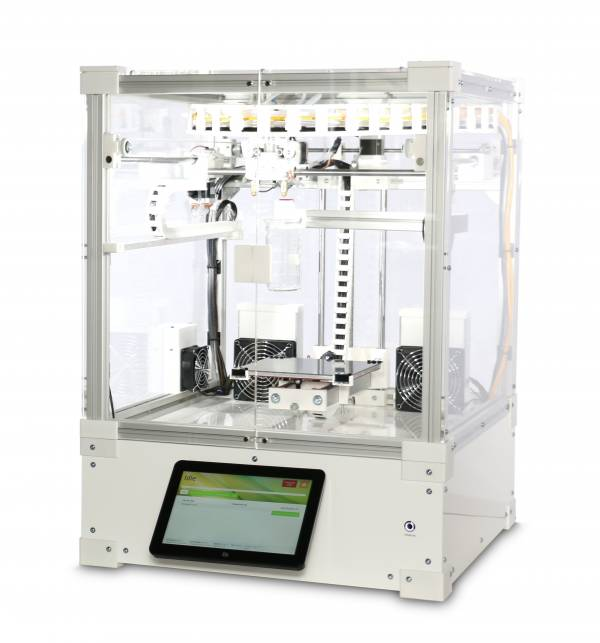
\includegraphics[width=.7\linewidth]{./img/ht500_freigestellt.jpg}
  \vfill
  \par\large Published \today
\end{titlepage}

% LICENSE INFORMATION
\clearpage
\thispagestyle{empty}
\mbox{}
\vfill
\begin{center}
Copyright (C) 2018 Kühling\&Kühling GmbH.

Permission is granted to copy, distribute and/or modify this document
under the terms of the GNU Free Documentation License, Version 1.3
or any later version published by the Free Software Foundation;
with no Invariant Sections, no Front-Cover Texts, and no Back-Cover Texts.
\end{center}

% TABLE OF CONTENTS
\clearpage
\pagenumbering{arabic}
\tableofcontents

% MANUAL CONTENT
\clearpage
\pagenumbering{arabic}
\section{General}

Welcome to the HT500.3 3D Printer operating manual of the Kühling\&Kühling GmbH (in the following referred to as \emph{Kühling\&Kühling}).
The HT500.3 3D Printer (in the following referred to as \emph{HT500.3} or \emph{3D Printer}) is a fully automatic stand-alone device for 
\emph{F}used-\emph{F}ilament-\emph{F}abrication (FFF) in a lab or commercial environment.
Any information needed for installing and commissioning, operating, troubleshooting, maintenance and repair of the 3D Printer are described in this document.
This user's manual must be read thoroughly as it is meant to provide the operator with all information needed to operate the HT500.3 safely and reasonably. Please always provide access to the document for any user of the 3D Printer in case of questions or problems. 

\begin{info}
  The HT500.3 3D Printer is an Open Source Hardware product. Any alteration, structural and design changes or customization for test reasons, optimization and improvement are encouraged by Kühling\&Kühling. We would like to support you with your advancements and are looking forward to receiving your feedback. We will always consider letting your achievements slip in to constantly improve the HT500.3. However, please note that Kühling\&Kühling cannot be held liable for damages and injuries resulting from such alterations 
  (see Intended use also).
\end{info}



\subsection{Valid Version}


\subsubsection{Hardware revisions}

\begin{table}[H]
  \centering
  \begin{tabulary}{\textwidth}{ L L L }
    \toprule
    Number of revision\\
    \midrule
    \hardwarerevision \\
    \bottomrule
  \end{tabulary}
\end{table}

 On the type plate at the rear side of the HT500.3 you find all information to precisely identify your 3D Printer:

\begin{itemize}
  \item Serial number
  \item Date of manufacturing
  \item Hardware Revision\footnote{You will also find the valid hardware revision in the \lbrack Setup\rbrack  menu on the touchscreen.}
\end{itemize}

\begin{figure}[H]
  \centering
  
\includegraphics[width=.7\linewidth]{./img/type_plate_ht500-3.png}
  \caption{Type plate on the rear side.}
\end{figure}


\subsubsection{Software versions}

Operating sofware:
RepRapOnRails Version v2.x.x $\rightarrow$ Operating manual



\subsection{Intended use}

The HT500.3 3D Printer has been designed and built for printing three-dimensional workpieces of nearly random geometries from common 2.85 mm 
thermoplastic filament strands.
The 3D Printer features advanced hot-ends with an extrusion temperature up to 500\degree C. 
In combination with the heated build chamber (up to 70\degree C) and the heated print bed (up to 130\degree C), this makes the HT500.3 
suitable for printing a vast scope of materials. It is therefor capable of performing regular 3D printing tasks with standard thermoplastics
as well as special jobs with a variety of technical plastics.
Contact \emph{Kühling\&Kühling} or refer to our web shop for more detailed information on available and applicable materials.

The HT500.3 is intended for industrial and commercial use. It is not valid for the operation in an explosive atmosphere.
Observing this manual and adhering to the stated information is part of the proper operation.
Improper operation of the HT500.3 can lead to hazardous situations.
It is forbidden to operate the 3D Printer under conditions and for purposes other than stated in this manual.

Operating the HT500.3 is forbidden under the following circumstances: 

\begin{itemize}
  \item The HT500.3 is used for a purpose not designated.
  \item The HT500.3 or single parts are damaged, the electrical equipment has been installed improperly, or the isolation is defective.
  \item The HT500.3 does not function flawless.
  \item Mechanical components or the control system have been inexpertly altered or reconstructed.
  \item Operating parameter have been altered inadmissibly.
  \item Operation with unspecified materials.
  \item Use of unspecified tools.
  \item Failure to regularly perform the prescribed maintenance work.
  \item Operation in an explosive atmosphere.
\end{itemize}



\subsection{Warranty terms}

The general terms and conditions of Kühling\&Kühling GmbH apply. The customer is familiar with these terms latest on the day of signing the purchase contract.

The warranty terms and the liability period can be found in the contract documents and in the order confirmation.

Warranty claims and liability are voided in one or more of the following applies:

\begin{itemize}
  \item unintended usage of the HT500.3
  \item false setup, commissioning, operation repair or maintenance
  \item operating the apparatus with defective, missing, improperly installed and/or malfunctioning equipment.
  \item unauthorized or inadmissible alteration of the electrical or mechanical equipment or the operating parameters of the apparatus.
  \item use of other than the specified replacement parts, tools, and/or operating materials
  \item exceeding the specified maintenance intervals
  \item cases of disaster and force majeure
\end{itemize}

\begin{info}
  Any unintended use or structural alteration of the HT500.3 not agreed upon with and approved in writing by Kühling\&Kühling render the warranty and the EU Declaration of Conformity void and free Kühling\&Kühling from product liability. Even if approved, alterations have to be carried out by the customer thoroughly and properly. If necessary, adequate safety devices have to be installed. 
\end{info}



\subsection{Ordering wear and spare parts and material}

Wear parts must meet the technical specifications defined by \emph{Kühling\&Kühling}. \emph{Kühling\&Kühling} original parts are subject to rigid requirements and meet these standards. A complete list of available wear and spare parts and suppliable materials can be requested from \emph{Kühling\&Kühling}. 



\subsection{Imprint}

Kühling\&Kühling GmbH\\
Christianspries 30\\
24159 Kiel\\
Deutschland\\
E-Mail: office@kuehlingkuehling.de\\
Tel.: +49 (0) 431 98 35 24 73\\
\\
Local Court: Amtsgericht Kiel\\
Commercial Register No.: HRB 17535\\
Managing Directors: Jonas Kühling, Simon Kühling, Karsten Wenige\\
VAT Reg.No.: DE305873054\\

\section{Safety}



\subsection {Personnel safety and device reliability}

The HT500.3 features state-of-the-art design and construction and has been built and tested thoroughly so that it is safe and ready to use at delivery. Nonetheless, hazardous situations may appear due to the production process itself and property damage may be caused by false operation.

\emph{The risk of experiencing hazardous situations is increased by:}

\begin{itemize}
  \item Using the HT500.3 for other applications than the intended.
  \item Inappropriate usage of the 3D Printer.
  \item Operating the 3D Printer in a non-safe state or under improper conditions.
  \item Insufficient attention, lax handling or intensive soiling.
\end{itemize}

\emph{Therefore:}
\begin{itemize}
  \item Use the HT500.3 for its intended use only.
  \item The HT500.3 must be in goor working order and in a safe state at any time. Check the apparatus prior to every commissioning
        and at regular intervals for wear, damage and cleanliness.
  \item Ensure that nobody can be injured by parts of the 3D Printer.
  \item Fix any error condition or visible damage immediately. If prompt rectification is impossible, 
        decommission the 3D Printer and do not put it back to use unless all problems have been solved.
  \item Regard the local accident prevention regulation.
  \item Provide access to the operating manual for anybody operating the machine.
\end{itemize}

\begin{info}
  The manufacturer cannot be held liable for injuries and damages due to inappropriate usage of the HT500.3.
  Inappropriate usage of the HT500.3 voids the manufacturer's warranty.
\end{info}



\subsection{Injury risks}

Some hazards are design related and cannot be avoided by mere constructive measures. To avoid injuries it is necessary that the operator is aware of such situations and takes adequate care. It is the owners responsibility to ensure that every user of the 3D Printer is informed about risks and preventions and that the safety precautions are observed. Access to this manual must be provided at all times.
The safety advice given in the following is meant to protect the operator of the HT500.3.


\subsubsection{Electrical safety}

The HT500.3 is operated with 110 to 230 V (DC). 
Touching current-carrying parts can be \emph{life-threatening} and cause \emph{severe injuries}.

\begin{itemize}    
  \item Only connect the 3D Printer in accordance with the specifications given in the data sheet.
  \item Works on the electrical equipment of the HT500 and on the power supply system may \emph{only} be carried out by skilled electricians.
  \item Always disconnect the 3D Printer from the power supply by switching the main switch off and removing the mains plug from the socket 
        before carrying out maintenance, repair or cleaning.
  \item Check the condition of cables and isolations at regular intervals and replace damaged parts immediately.
  \item Do not setup and operate the 3D Printer in a humid environment.
\end{itemize}


\subsubsection{Hot surfaces}

Outer surfaces of the HT500.3 are adequately isolated and do not exceed temperatures of +40\degree C (104\degree F). They are safe to the touch at any time.
Inside the build chamber, the heating elements generate the necessary ambient temperature for warp-free printing.
Depending on the processed material, surfaces inside the build chamber can \emph{reach temperatures up to +70\degree C (158\degree F)}.
The print table is heated separately, also to minimize warpage. It can \emph{reach temperatures up to 130\degree C (266\degree F)}.
The extruder nozzles are heated to melt the filament strands and may \emph{reach temperatures of 500\degree C (932\degree F)}.

Touching heated components may lead to grade 1 burning injuries, in case of the nozzles of grade 2 of limited size.

To avoid burning injuries:

\begin{itemize}
  \item \emph{Do not open} the build chamber during or immediately after completion of a print job.
  \item \emph{Always switch off} the preheating and wait until the print bed temperature indicated on the touchscreen 
        has dropped below 50\degree C (122\degree F) 
        before removing the print bed. This is also to avoid stress cracks due to sudden temperature drop.
  \item Some tasks require handling at operating temperature. Wear adequate protective gloves when handling 
        hot components.
  \item Observe the procedures and waiting times stated in this manual.
\end{itemize}


\subsubsection{Coolant}

For proper operation the HT500.3 is equipped with a closed loop low-maintenance cooling system that needs little interference. The circuit is filled with coolant type \emph{Innovatek Protect IP ready-to-use}.
If it is necessary to perform works on the cooling system, such as refilling coolant or exchanging defective hoses, avoid direct skin or eye contact. Always wear \emph{adequate protective gloves} that are resistant to chemical substances (e.g. PVC, NBR).
Observe the information provided in the manufacturer's safety data sheet.
Additional information concerning the cooling system and required maintenance can be found in the Service Guide.


\subsubsection{Noise}

The HT500.3 3D Printer is build to be operated in a professional environment such as workshops and laboratories. It is not suited for the operation in an office. During print jobs, it does not exceed 60dB(A), which is considered “unauspicious” for long-term exposure.
Special noise protection equipment is not required.


\subsubsection{Fumes}

Molten plastics may emit unpleasantly smelling fumes. Such fumes can be \emph{perilous}.
It is vitally important not to exceed the temperature limits stated for a printed material. Overheating is indicated by discoloration and coking.


\subsubsection{Emergency stop}

You will find a red \emph{Emergency STOP} button in the top-right corner of the touchscreen. In case of any unexpected performance of the 3D Printer, press this button to immediately stop any mechanical movement in the build chamber and to shut down all heater elements.

\begin{notice}
  The emergency stop function does not provide a cool down sequence. Do not use the emergency stop button to abort current print jobs, because this may lead to damage of the 3D Printer due to uncontrolled heat accumulation.
  Do not use the main switch as an emergency stop button. You risk loosing or corrupting data. 
\end{notice}

When the emergency stop is triggered, the microcontroller board responsible for the stepper motors, heaters and sensors is reset immediately and returns to idle state afterwards. Now it is safe to resolve any problems or defects in the build chamber.

The build chamber can then be reactivated via the \lbrack Print\rbrack  menue.
Detailed information are provided in the Operating manual. 

\begin{figure}[H]
  \centering
  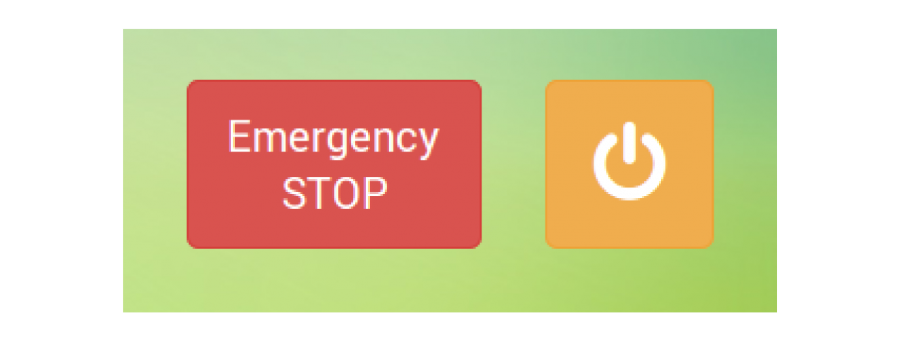
\includegraphics[width=.7\linewidth]{./img/gui_v110_emergencystop.png}
  \caption{The emergency stop button in the top-right corner of the GUI will immediately stop all movement and set the 3D Printer in a safe 
           state for troubleshooting.}
\end{figure}


\subsubsection{Operator qualification}

Operating and service personnel must be familiar with the information provided in the manual. Special training and qualification are not required for operating the 3D Printer. Works on the electrical equipment and connections of the 3D Printer require profound knowledge of electrics and electronics.


\subsubsection{Personal protective equipment}

During normal operation it is not necessary to wear special protective gear. Some tasks however should not be performed without taking protective measures. Situations that require protective equipment are specially indicated. It is the owner's obligation to provide adequate protective equipment.


\subsubsection{Product reliability}

False handling of components can lead to loss of production due to property damage; therefore we strongly recommend following the information given in this manual.


\subsubsection{Print head nozzles}

The stainless steel print head nozzles are sensitive to heat treatment and mechanical strain.
If the nozzles or extruder barrels are clogged by congealed material, reheating during the normal production flow is utterly sufficient to clear them in most cases.
In case you want to change the material type or clogging is effected by foreign particles (i.e. dust grains dragged along with the filament), it is necessary to remove congealed material from the nozzles. The corresponding description can be found in the cleaning recommendation.

\begin{notice}
  Do not use mechanical tools or open flames to remelt or remove residues in the nozzles. Overheating may induce easing of tensions and deformation. The nozzle is then no longer usable for printing.
\end{notice}

\section{Description}

The following paragraphs name and explain all components of the HT500.3 to give you an exact overview. The terms are used consistently throughout this manual and will help you identify any part you may wish to find or order as a spare part. 



\subsection{Functional principle}

The HT500.3 3D Printer uses the \emph{F}used \emph{F}ilament \emph{F}abrication (FFF) process to build up workpieces in subsequent layers of 0.10 to 0.60mm thickness. The plastic filament is heated in the nozzle to its melting temperature and continuously conveyed by a cogwheel. The molten plastic is pressed through the bore of the nozzle tip and onto the heated print bed. After each layer the print bed is lowered by the preset layer height and the next layer is applied. The heat of the newly applied plastic ensures an adequate binding of the layers.

All temperatures and movement commands are provided by the GCODE, a file format previously generated with a \dq slicing\dq software. This file contains all information for a single print job and is uploaded to the 3D Printer via the web interface.

After the workpiece has been finished the user can leave it in the heated build chamber to slowly cool down thus reducing shrinkage and internal tensions, or he can immediately remove it and start the next print job. The layered building process enables the user to create even complex forms that otherwise could not be realized. 

\begin{figure}[H]
  \centering
  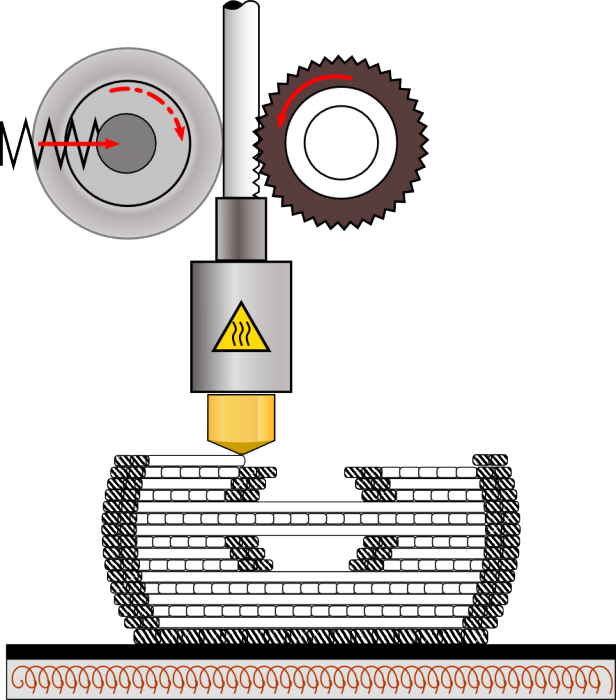
\includegraphics[width=.7\linewidth]{./img/fff_principle_manual.png}
  \caption{The layer-by-layer build-up of random geometries becomes possible with FFF-3D Printers.}
\end{figure}



\subsection{Hardware components}

The HT500.3 is built on an aluminum framework covered with acrylic panels. Its main functional sections are the upper build chamber and the lower electronic chamber. The build chamber is covered with translucent plates to provide insight during production. It contains all mechanical components. At the back cover, the filament supply is installed.

The lower chamber is covered with opaque sheets and contains the electronic components and the mains adapter. All connections and the power switches are located here and the touchscreen for operation is mounted at the front cover.

All covers are fixed to the frame with M4x20 hexagon socket screws and hammerhead nuts, thus being easy to remove and making all around access possible to all parts if required. 

\begin{figure}[H]
  \centering
  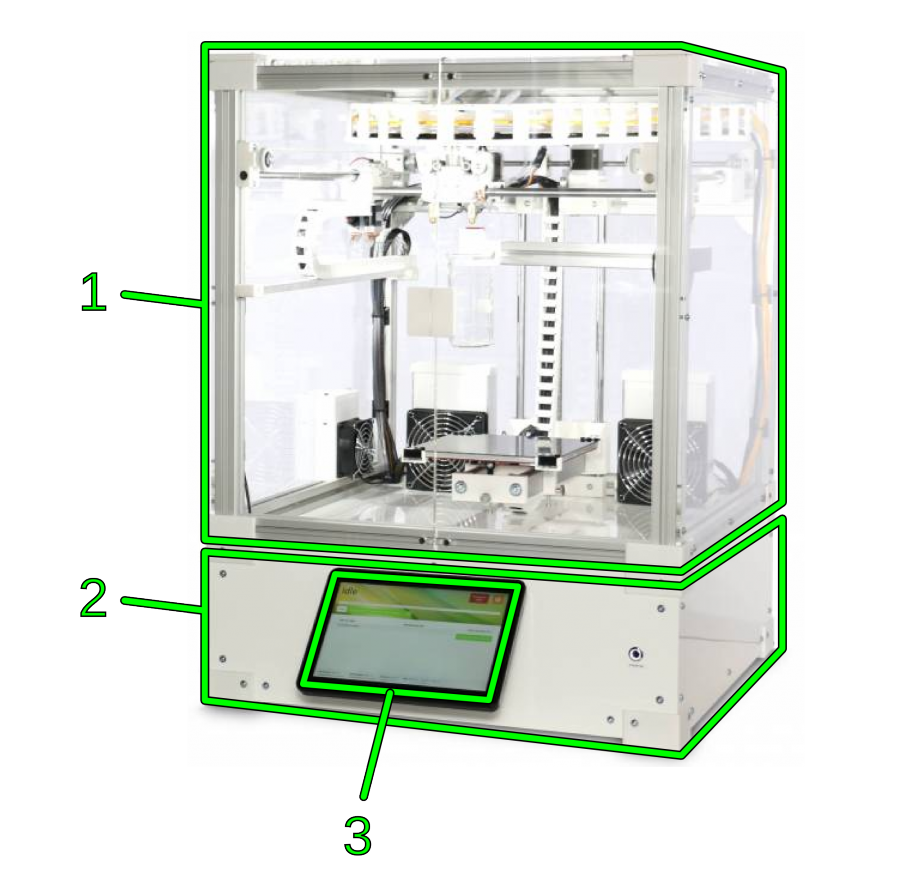
\includegraphics[width=.7\linewidth]{./img/desc_main_1.png}
  \caption{General overview of the HT500.3 3D Printer.}
\end{figure}

\begin{table}[H]
  \centering
  \begin{tabulary}{\textwidth}{ L L }
    \toprule
    No.   &   Description  \\
    \midrule
      1     & Build chamber \\
      2     & Electronic chamber \\
      3     & Touchscreen  \\
    \bottomrule
  \end{tabulary}
\end{table}

All references concerning directions are defined throughout this manual as follows:

\begin{figure}[H]
  \centering
  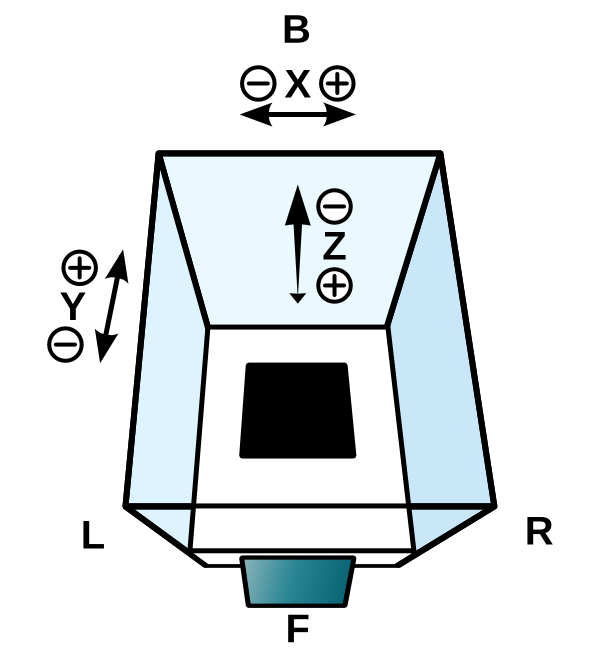
\includegraphics[width=.7\linewidth]{./img/directions_ht500.png}
  \caption{Directions and aspects of the 3D Printer. All statements refer to the frontal view.}
\end{figure}

\begin{table}[H]
  \centering
  \begin{tabulary}{\textwidth}{ L L L }
    \toprule
    Tag      & 	Aspect     &	Description \\
    \midrule
      F 	   &  Front      &	Standing in front of the 3D Printer's touchscreen and looking inside the build chamber. 
                              This is the reference view for all other directions.\\
      L      &	Left       &	Left side of the 3D Printer, referred to the frontal view.\\
      R 	   &  Right      &	Right side of the 3D Printer, referred to the frontal view.\\
      B      &	Back       &	Backside of the 3D Printer, referred to the frontal view.\\ 
    \bottomrule
  \end{tabulary}
\end{table}

All movement directions of the axes are defined throughout this manual as follows: 

\begin{table}[H]
  \centering
  \begin{tabulary}{\textwidth}{ L L L }
    \toprule
    Tag                & 	Called &  	Movement direction \\
    \midrule
    X \textcircled{+}  & 	X positive  &  	Extruder head moves to the right.\\
    X \textcircled{-}  & 	X negative  & 	Extruder head moves to the left.\\
    Y \textcircled{+}  &  Y positive  & 	Extruder head moves backwards.\\
    Y \textcircled{-}  & 	Y negative  & 	Extruder head moves forward.\\
    Z \textcircled{+}  & 	Z positive  &  	Print table moves down.\\
    Z \textcircled{-}  & 	Z negative  & 	Print table moves up. \\
    \bottomrule
  \end{tabulary}
\end{table}

All movements of the extruder drives are defined throughout this manual as follows: 

\begin{figure}[H]
  \centering
  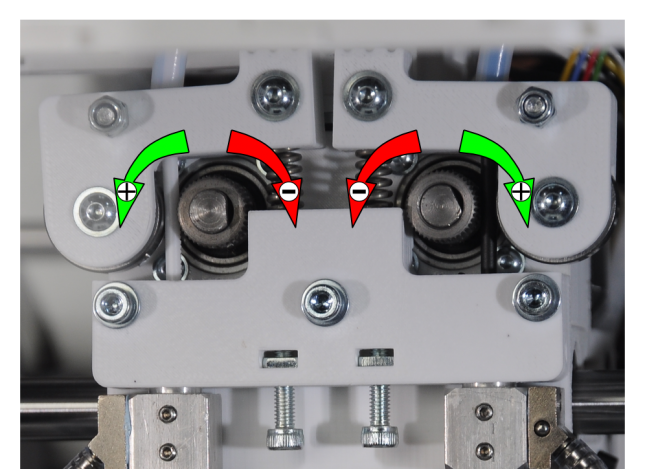
\includegraphics[width=.7\linewidth]{./img/desc_moving_drives.png}
  \caption{Movement directions of the extruder drives.}
\end{figure}

\begin{table}[H]
  \centering
  \begin{tabulary}{\textwidth}{ L L L }
    \toprule
    Tag             &   Called      & Movement direction \\
    \midrule
    \textcircled{+} &	extrude     & Left extruder $\rightarrow$ counter-clockwise rotation\\
                    &               & Right extruder $\rightarrow$ clockwise rotation\\
    \textcircled{-} &	retract     & Left extruder$\rightarrow$ clockwise rotation \\
                    &               & Right extruder $\rightarrow$ counter-clockwise rotation \\
    \bottomrule
  \end{tabulary}
\end{table}


\subsubsection{Build chamber}

\begin{figure}[H]
  \centering
  \includegraphics[width=.7\linewidth]{./img/desc_buildchamber_insideview.png}
  \caption{Inside view of the build chamber.}
\end{figure}

\begin{table}[H]
  \centering
  \begin{tabulary}{\textwidth}{ L L }
    \toprule
    No.  & 	Description \\
    \midrule
      1  & 	Extruder head \\
      2  & 	Print table \\
      3  & 	Heating elements (covered) and fans \\
    \bottomrule
  \end{tabulary}
\end{table}

The build chamber is the main production area with a vertically moving print table and a two-directional horizontally moving extruder head inside.
All electrical motors are installed at their working point and equipped with a water cooling system. The extruder head moves on an H-frame, tooth-belt-driven by two separate stepper motors in X- and Y-direction. The print table is lifted and lowered in Z-direction by a spindle drive.
For regulating the temperature inside the build chamber two heating resistors in separate housings heat the air which then is circulated through the chamber by the fans.
Cables and hoses are installed in and guided by cable carriers.
The access to the build chamber is the magnetically closed double door at the front. 

\begin{figure}[H]
  \centering
  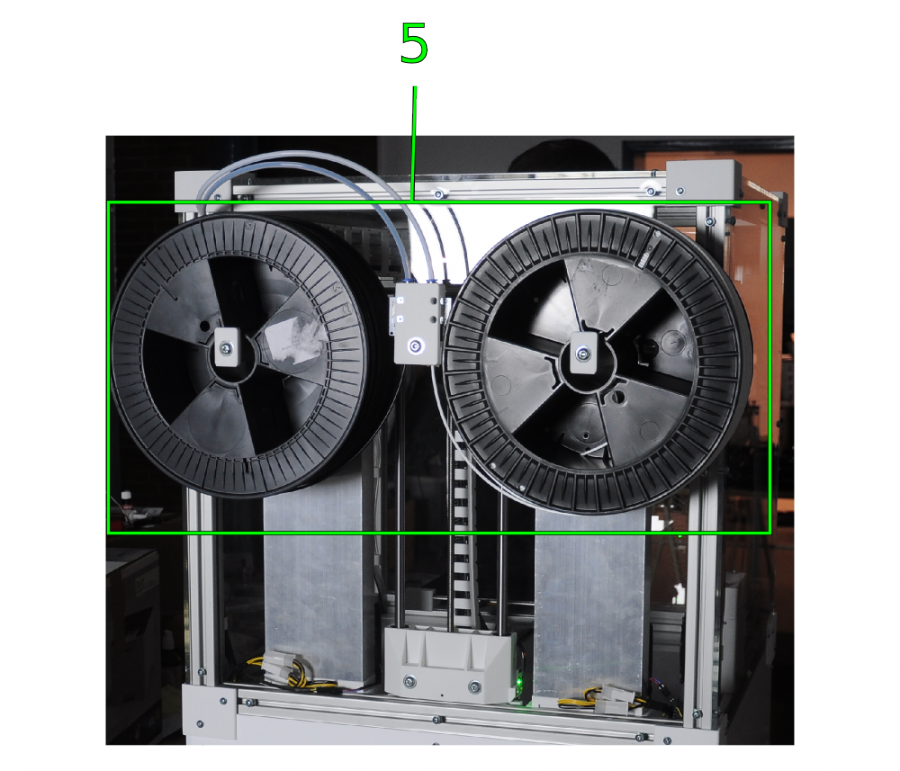
\includegraphics[width=.7\linewidth]{./img/desc_buildchamber_backview.png}
  \caption{Filament supply unit at the rear side of the build chamber.}
\end{figure}

\begin{table}[H]
  \centering
  \begin{tabulary}{\textwidth}{ L L }
    \toprule
    No.  & 	Description \\
    \midrule
      5  &	Filament supply \\
    \bottomrule
  \end{tabulary}
\end{table}

The filament spools that provide the necessary material are installed at the rear of the build chamber next to the filament feed unit.

\subsubsection{Print head components}

\begin{figure}[H]
  \centering
  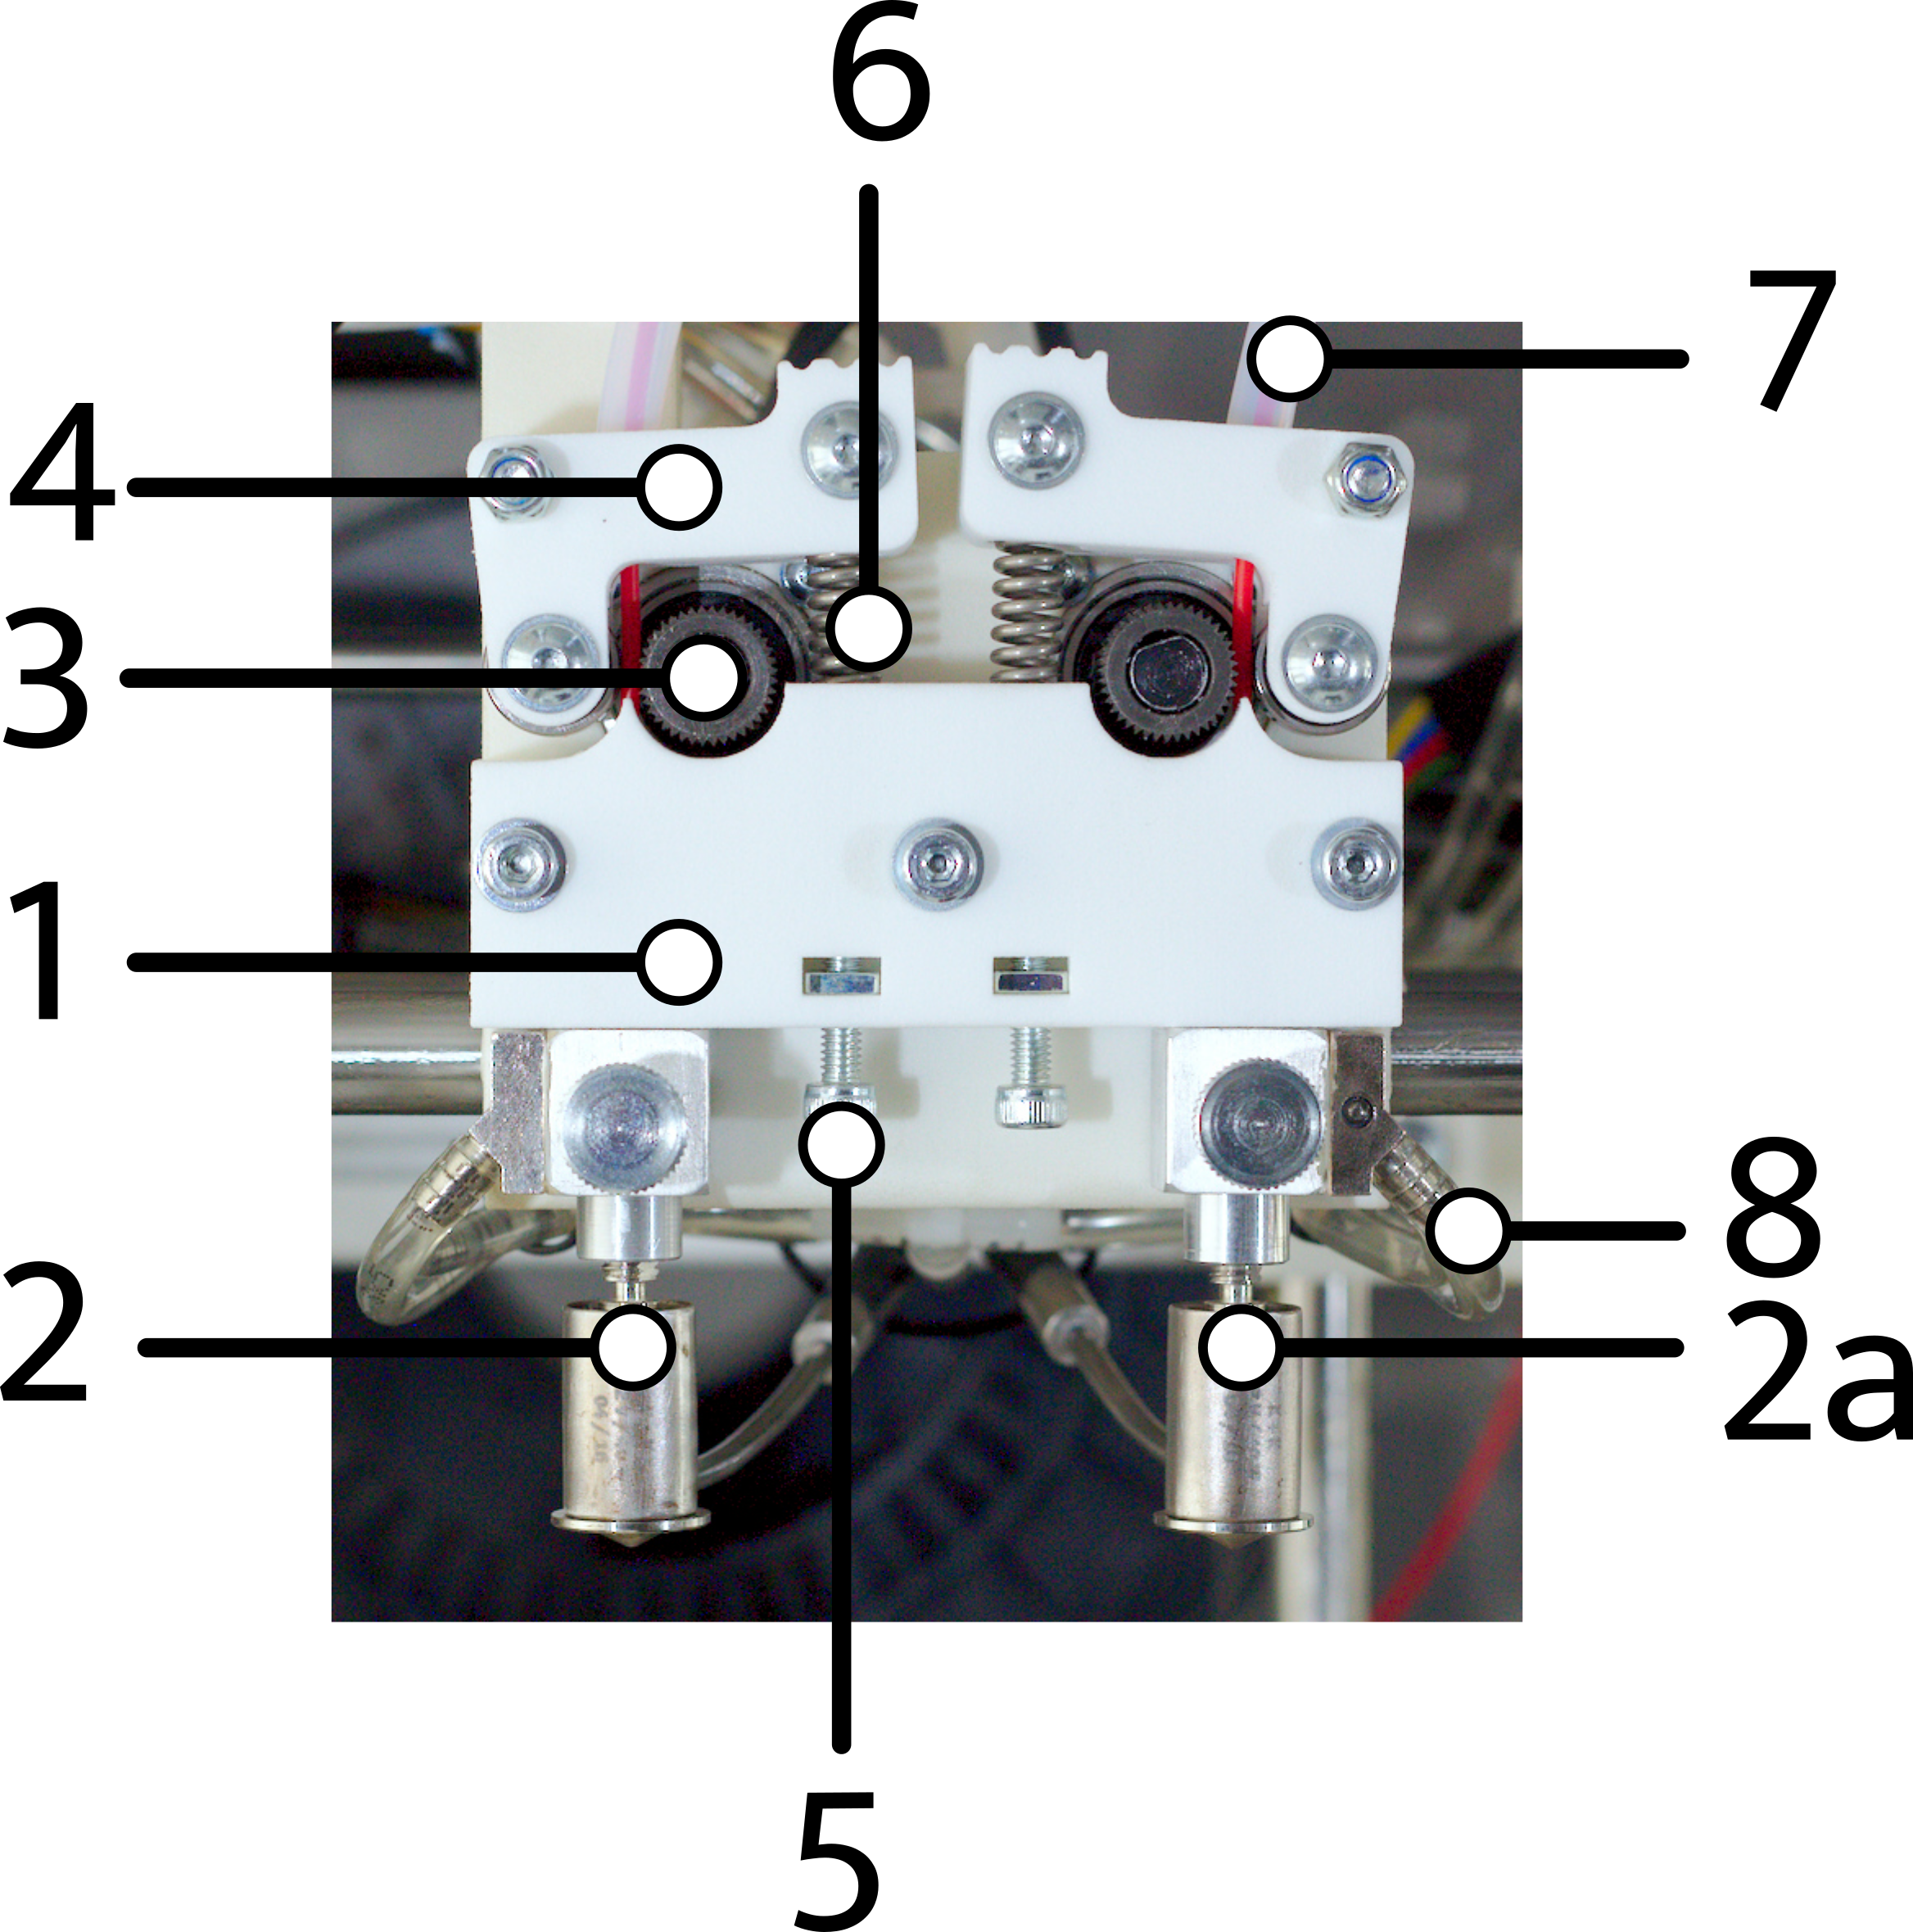
\includegraphics[width=.7\linewidth]{./img/desc_extruderhead.png}
  \caption{Extruder head components}
\end{figure}

\begin{table}[H]
  \centering
  \begin{tabulary}{\textwidth}{ L L }
    \toprule
    No.  & 	Description \\
    \midrule
      1  &	Carriage \\
      2  &  Left (primary) hot end \\
      2a &	Right (secondary) hot end \\
       3 &	Filament drive gear \\
       4 &	Idler lever (release function)\\
       5 &	Spring tensioning screw M4x20 \\
       6 &	Idler spring \\
       7 &	Filament feed hose \\
       8 &	Cooling hoses \\
    \bottomrule
  \end{tabulary}
\end{table}

The extruder head is mounted to the traverse of the H-frame and moves horizontally in X- and Y-direction with useful operating ranges of X = 200 mm and Y = 185 mm.
It contains the filament drive gears forwarding the filament strands and the hot ends which melt and dose the material onto the print table. The filament is supplied through a hose from the filament supply and is clamped between the idler lever and the filament drive gear. The filament drive gear is rotated by the filament feed motor and thereby forwarding the filament strand.
Each hot end is provided with its own filament strand, thus enabling bicolored prints, printing two materials or two objects simultaneously or printing with different extrusion thicknesses (e.g. for outer contours and inner filling structures).

\begin{figure}[H]
  \centering
  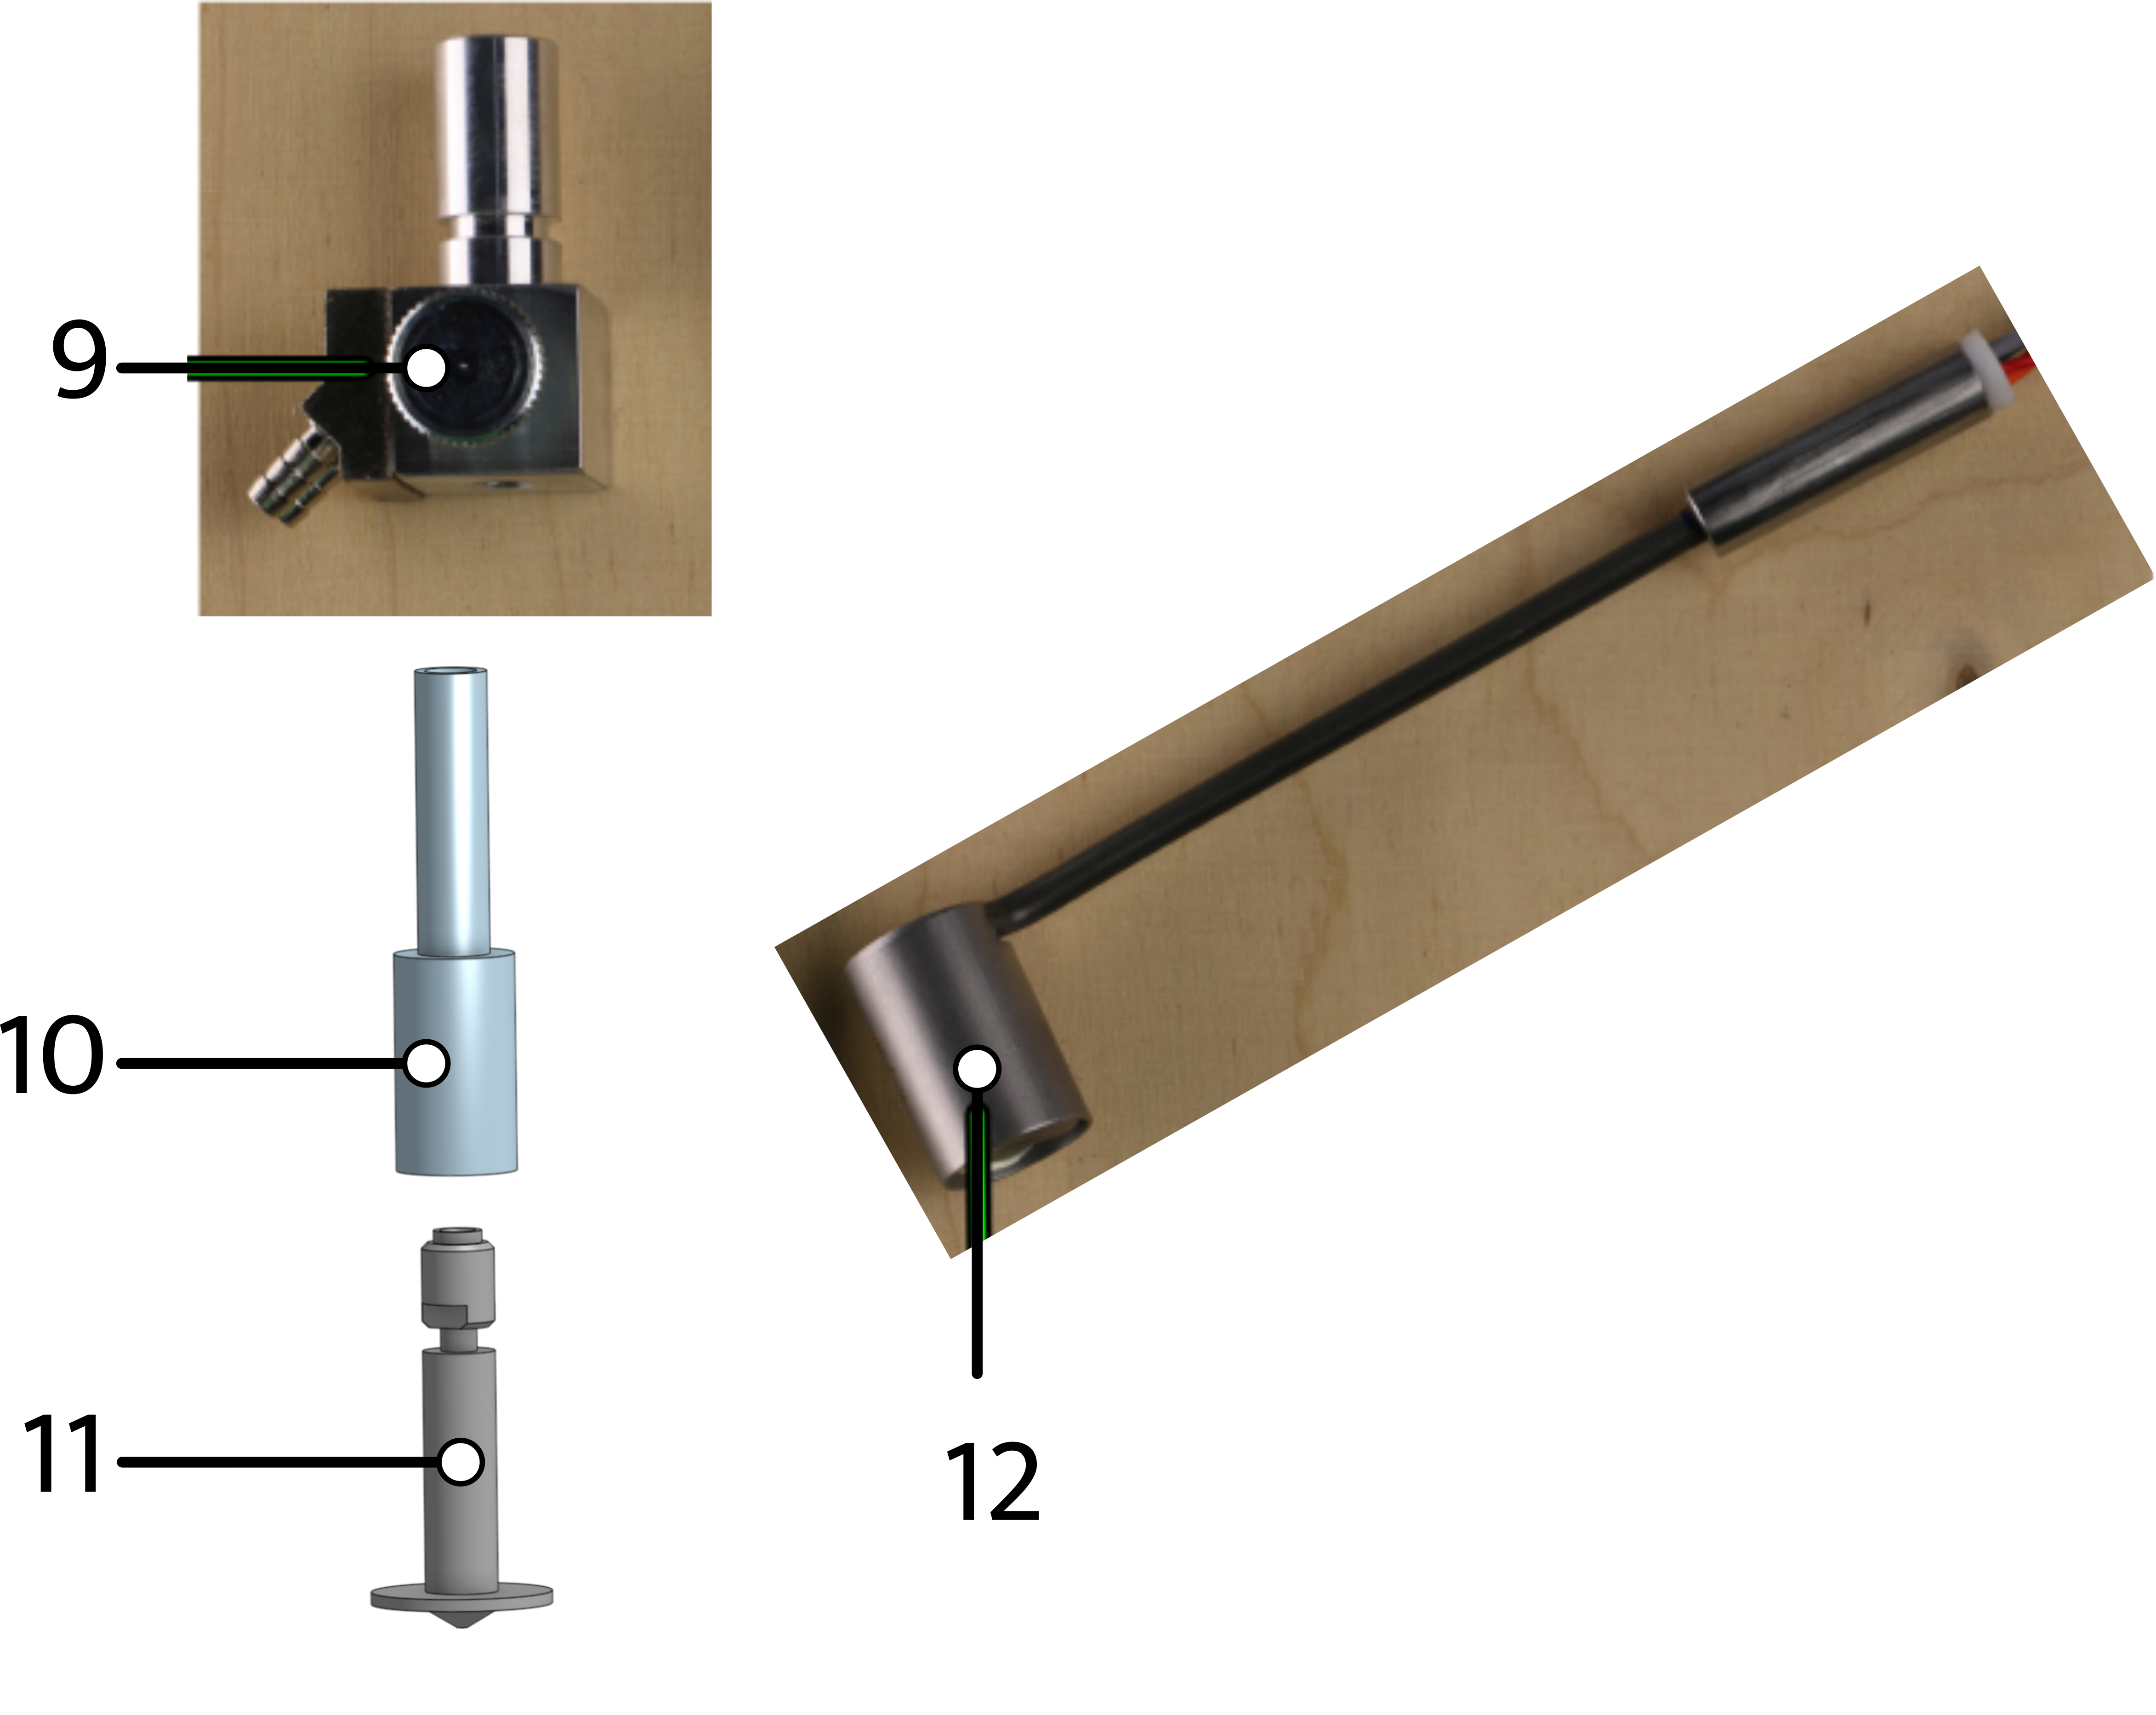
\includegraphics[width=.7\linewidth]{./img/desc_extruderheadcomponents.png}
  \caption{Extruder head components}
\end{figure}

\begin{table}[H]
  \centering
  \begin{tabulary}{\textwidth}{ L L }
    \toprule
    No.  & 	Description \\
    \midrule
     9 &	Aluminum hot-end mount (cooling block) with thumb screw and cooling hose adapter\\
    10 &	Nozzle Adapter\\
    11 &	Nozzle\\
    12 &	500\degree C heating cartridge with integrated thermocouple\\
    \bottomrule
  \end{tabulary}
\end{table}

Each hot-end is heated by a ceramic heating cartridge so that the filament is molten inside the nozzle. The integrated thermocouple provides direct alignment of set and actual temperature.
To improve the thermal control of the melting process the hot-end mount is connected to the cooling system, ensuring an even temperature distribution in a well defined area of the nozzles so that there is a preheating zone and a melting zone. 

\begin{figure}[H]
  \centering
  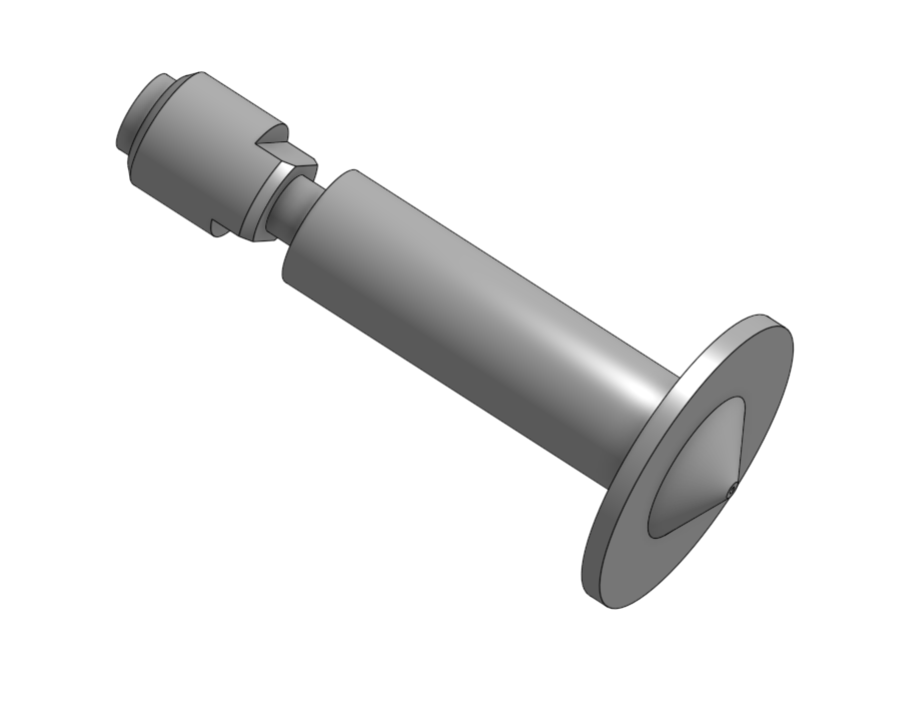
\includegraphics[width=.7\linewidth]{./img/desc_nozzle.png}
  \caption{A single nozzle.}
\end{figure}

The nozzle is exchangeable to provide different bore diameters for different materials, layer thicknesses or print speed. Ex factory, the 0.35mm tip is preinstalled on the left extruder and 0.5mm on the right extruder. Additionally, 0.75mm nozzles are available

\subsubsection{Print table and print bed}

The print table is mounted on the crossbeams of the elevator assembly which is positioned in Z-direction in its useful operating range by a spindle drive.

The print table itself consists of an aluminum sandwich panel with a silicone rubber heating pad, providing an even temperature distribution and ensuring optimal adhesion throughout the printing process. 

\begin{figure}[H]
  \centering
  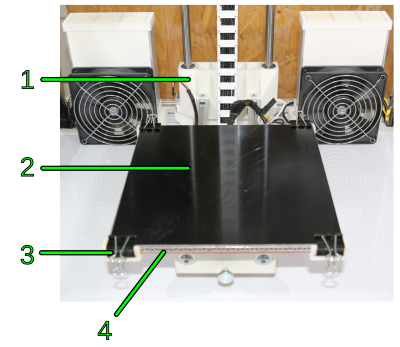
\includegraphics[width=.7\linewidth]{./img/print_table_overview.png}
  \caption{Print table and print bed fastened with four bulldog clamps}
\end{figure}

\begin{table}[H]
  \centering
  \begin{tabulary}{\textwidth}{ L L }
    \toprule
    No.  &  Description \\
    \midrule  
      1  &  Elevator assembly \\
      2  &  Removable PEI/ Carbon Fiber print bed \\
      3  &  Bulldog clamp \\
      4  &  Heated print table \\
    \bottomrule
  \end{tabulary}
\end{table}

It rests on three springs lockable with set screws for an even and accurate leveling since a precisely adjusted distance between print bed and nozzle tip is vital for the print bed adhesion an the print results.

The semi-automated leveling process is described in the Operating Manual.

Print jobs are executed on the removable print bed laid on the print table and fixed with four bulldog clamps at the corners. This fixation allows the use of print beds of different thicknesses.
The standard print bed included in the delivery is a 210x210x1.8mm polyetherimide (PEI) carbon fabric plate that provides excellent adhesion for a large variety of materials, including ABS, Nylon, PET, PC, HIPS, TPU and other. 

\begin{figure}[H]
  \centering
  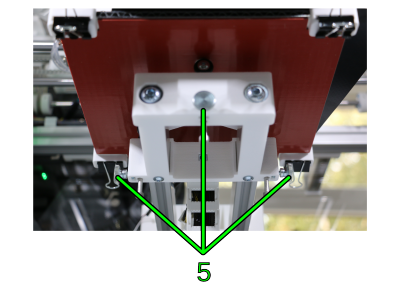
\includegraphics[width=.7\linewidth]{./img/print_table_overview_2.png}
  \caption{3-point leveling support}
\end{figure}

\begin{table}[H]
  \centering
  \begin{tabulary}{\textwidth}{ L L }
    \toprule
    No.  &  Description \\
    \midrule  
      5  &  Set screws of the spring-mounted 3-point leveling support \\
    \bottomrule
  \end{tabulary}
\end{table}

\paragraph{Important print bed knowledge}

The PEI carbon fabric composite print beds are, in accordance with the HT500.3's standards, optimized for printing ABS and are custom-made to Kühling\&Kühling specifications. It also works fine with HIPS, PET-Copolyester, PVA and thermoplastic urethane (TPE-U). Other materials may require a different subsurface, be it another material or a special treatment with tape or glue.

PEI is highly resistant to a lot of solvents which makes it a suitable subsurface for a lot of materials since removing residues and refurbishing for the next print becomes quite easy.

Find more information about the Kühling\&Kühling PEI print bed:

\begin{itemize}
  \item Operating and handling are described in the Operating manual.
  \item Cleaning and care can be found in the Service guide.
\end{itemize}


\subsubsection{Drives}

\begin{table}[H]
  \centering
  \begin{tabulary}{\textwidth}{ L L }
    \toprule
    No.  & 	Description \\
    \midrule  
    1    &	X-axis motor (extruder head motor) \\
    2    &	Y-axis motor (H-frame traverse motor) \\
    3    &	Z-axis motor (spindle drive of print table) \\
    4    &	Filament feed motors (filament gear drive) \\
    \bottomrule
  \end{tabulary}
\end{table}

Five electrical stepper motors, one per direction of the extruder head, one for lifting and lowering the print table and one per extruder head nozzle for forwarding the filament, provide all necessary movement for printing. All motors are equipped with water cooling to prevent overheating due to workload and the heating of the build chamber.

\begin{figure}[H]
  \centering
  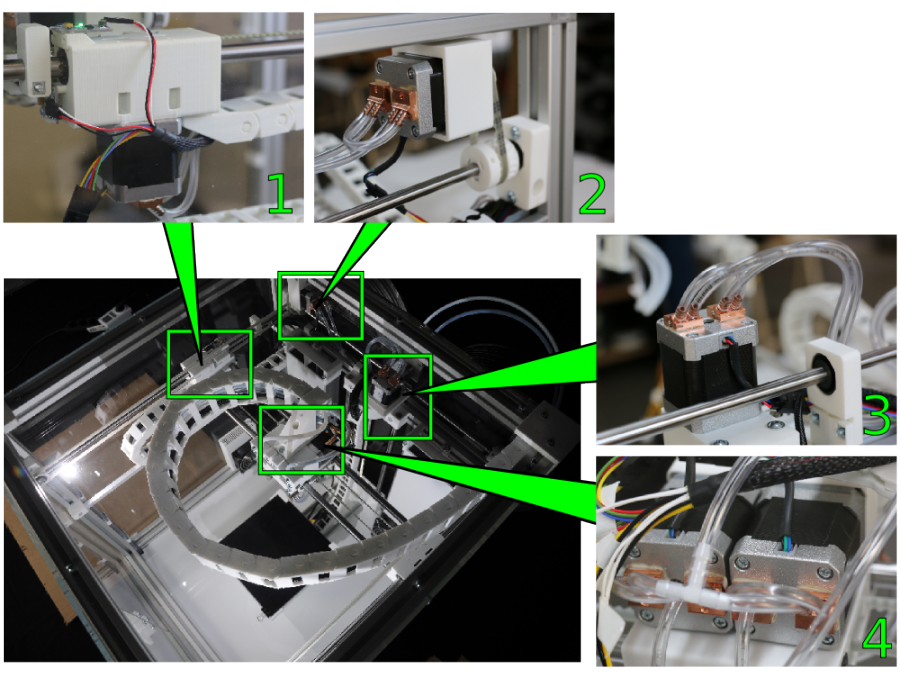
\includegraphics[width=.7\linewidth]{./img/desc_drives_2.png}
  \caption{Single views of the drive motors.}
\end{figure}


\subsubsection{Sensors}

Sensors for positioning and temperature control are installed inside the build chamber.

Every axis is equipped with a Hall effect sensor and a magnet for accurate home positioning. If the Hall effect sensor nears the magnet and measures the defined threshold value of the magnetic field strength, the sensor effects a \dq stop\dq signal via the machine controller. After all sensors have given this signal the moving axes are in home position. The home position is the reference value for all relative movement of the extruder head and the print bed.

\begin{figure}[H]
  \centering
  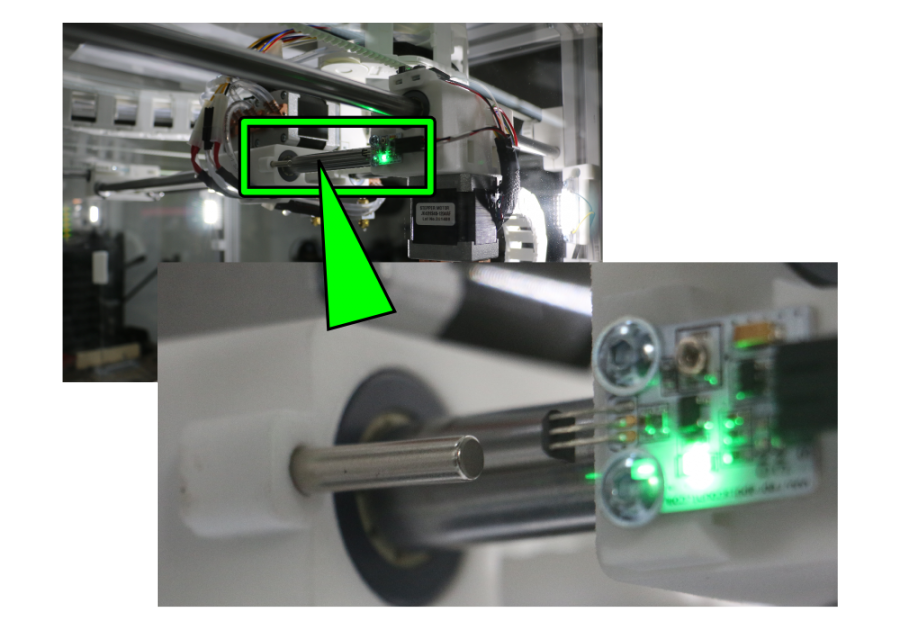
\includegraphics[width=.7\linewidth]{./img/desc_x-sensor.png}
  \caption{Hall effect sensor and magnet of the X-axis.}
\end{figure}

\begin{figure}[H]
  \centering
  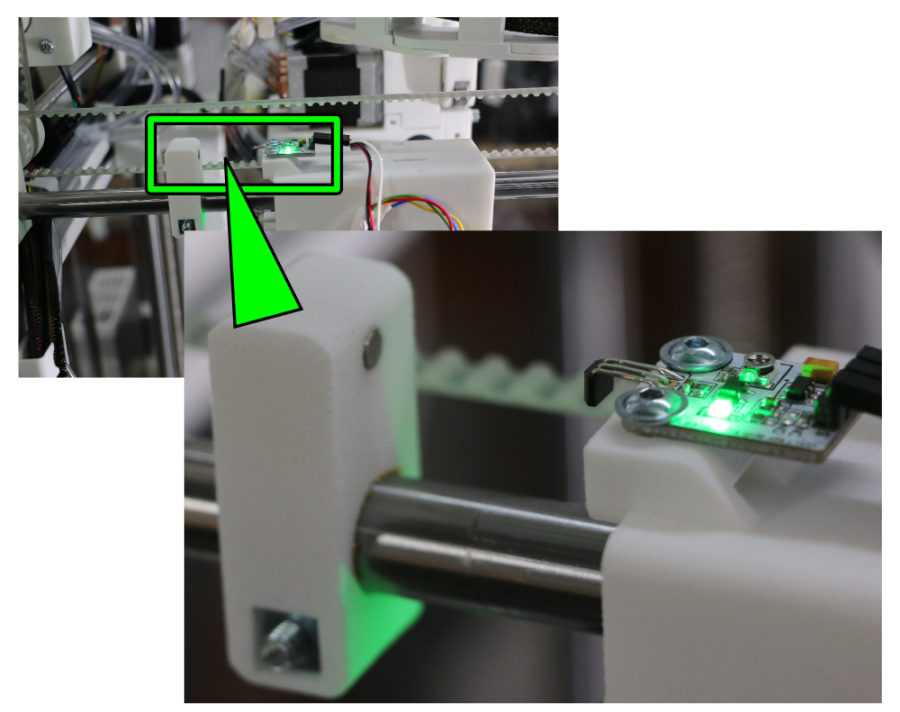
\includegraphics[width=.7\linewidth]{./img/desc_y-sensor.png}
  \caption{Hall effect sensor and magnet of the Y-axis.}
\end{figure}

\begin{figure}[H]
  \centering
  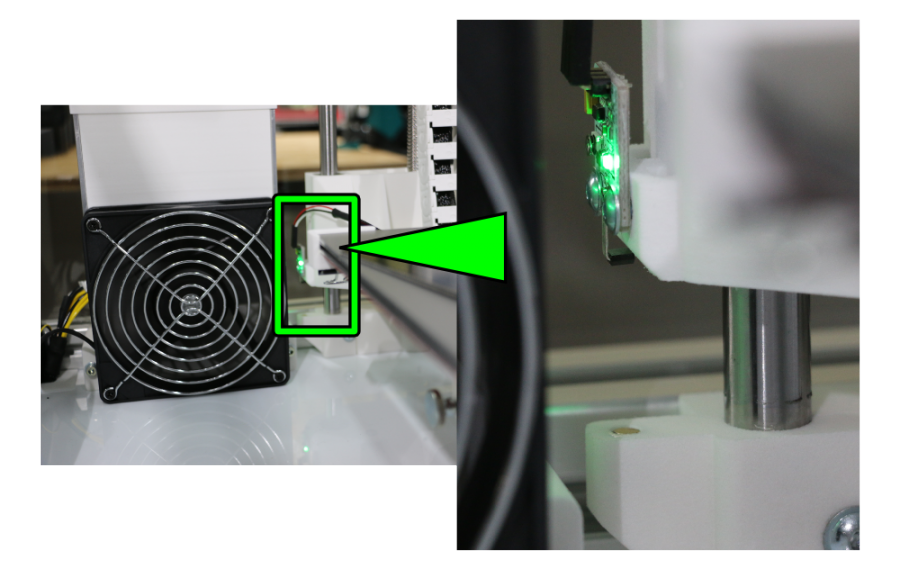
\includegraphics[width=.7\linewidth]{./img/desc_z-sensor.png}
  \caption{Hall effect sensor and magnet of the Z-axis.}
\end{figure}

Thermistors measure the relevant temperatures for the printing process, i.e. the print bed temperature and the build chamber temperature. 
All thermistors deliver their input signal to the machine controller and thus effect switching on and off the according heating resistor.

The print bed temperature is measured directly at the heating pad with which it is looped in a control circuit.
The build chamber sensor is installed at the elevator assembly and measures the air temperature inside the build chamber. Its measurements influence the control of the heating resistors inside the heating elements.

The extrusion temperature is measured directly at the heating cartridge by an integrated thermocouple.

\begin{figure}[H]
  \centering
  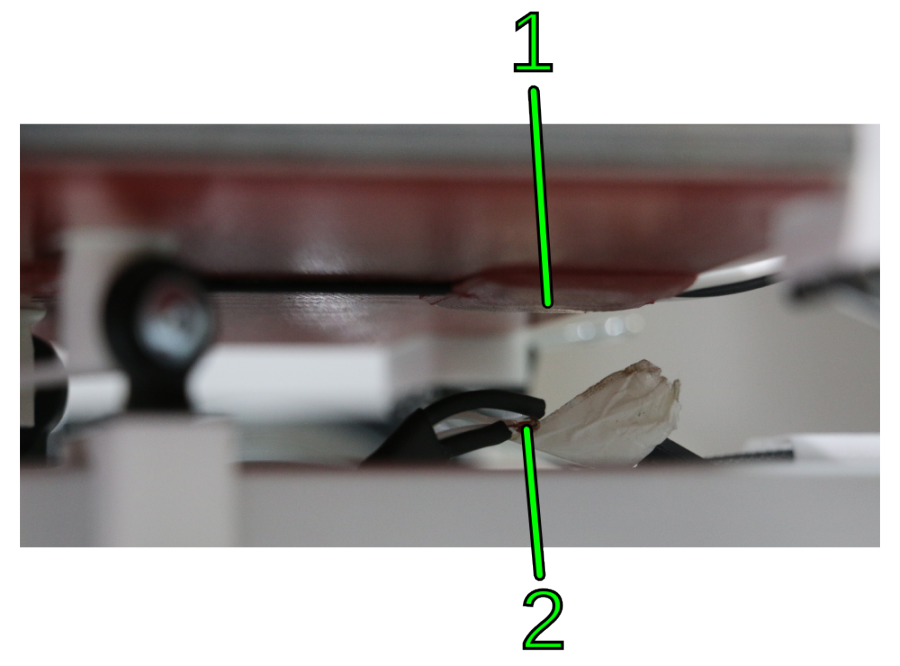
\includegraphics[width=.7\linewidth]{./img/desc_thermistors_printbed_chamber.png}
  \caption{Thermistors of the print bed (1) and the build chamber (2)}
\end{figure}

A limit switch is installed at every filament inlet of the filament feed unit
(see below). 


\subsubsection{Filament supply}

\begin{table}[H]
  \centering
  \begin{tabulary}{\textwidth}{ L L }
    \toprule
    No.  & 	Description \\
    \midrule  
    1    & 	Feed unit \\
    2    & 	Filament spool carrier \\
         & 	Filament spool (2.3 kg) \\
    4    & 	Limit switch \\
    5    & 	Filament inlet with dust wiping sponge \\
    \bottomrule
  \end{tabulary}
\end{table}

The HT500.3 is designed for printing filament strands of a diameter of 1.75 mm with a tolerance of $\pm$ 0.05 mm.
Two separate strands can be fed from the outside to the extruder head. One filament spool can be positioned on each spool carrier; a stop collar prevents them from falling off due to their rotation.
The end of the filament strand is manually inserted into the inlet of the feed unit and led through hoses to the two extruder nozzles. At the inlet the filament is put through a sponge that wipes dust off the strand to keep the material unsoiled before reaching the nozzle.
A limit switch registers the end of the filament strand when the spool is empty. The print process then is interrupted and the lack of material is signaled on the touchscreen. The printing process can be resumed after refilling the supply. 

\begin{figure}[H]
  \centering
  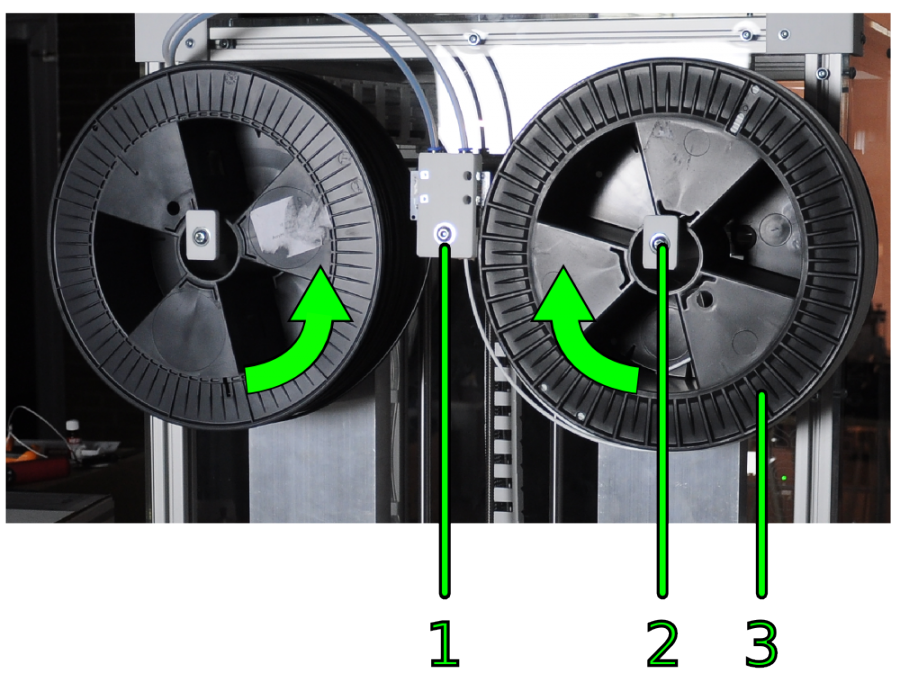
\includegraphics[width=.7\linewidth]{./img/desc_filamentfeedunit.png}
  \caption{Filament supply}
\end{figure}


\begin{figure}[H]
  \centering
  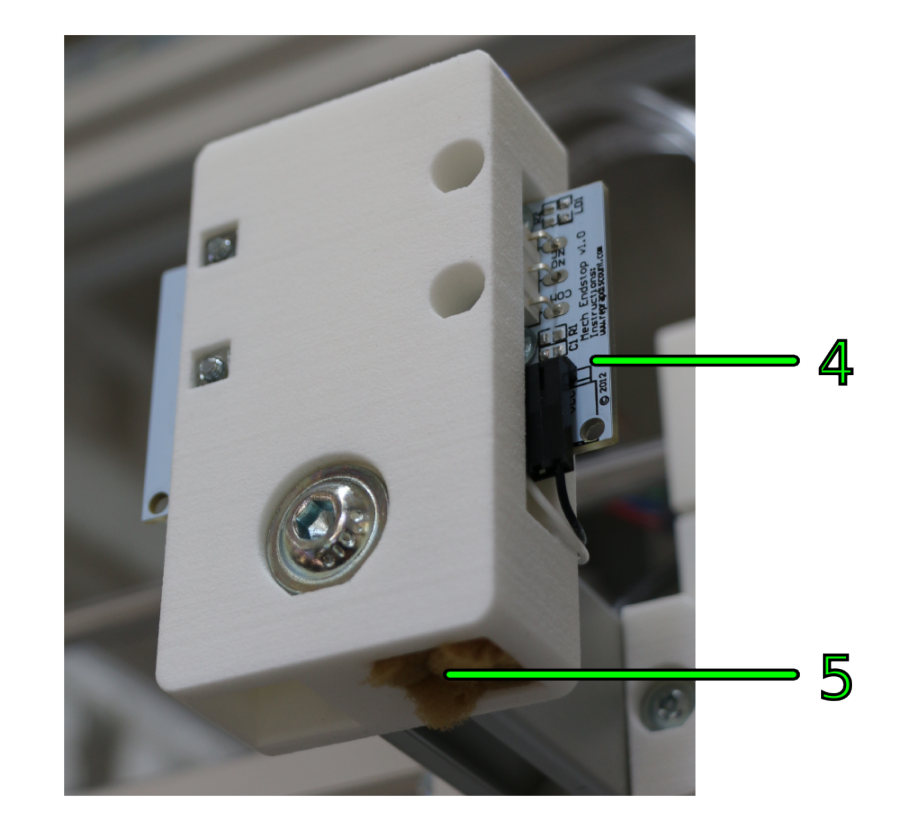
\includegraphics[width=.7\linewidth]{./img/desc_filamentfeedunit_dustsponge.png}
  \caption{Filament inlet with limit switch and dust wiping sponge.}
\end{figure}


\subsubsection{Wiper}

\begin{table}[H]
  \centering
  \begin{tabulary}{\textwidth}{ L L }
    \toprule
    No.  & 	Description \\
    \midrule  
    1    & 	Wiper lip \\
    2    & 	Bracket \\
    3    & 	Excess retainer \\
    4    & 	Mounting arm \\
    \bottomrule
  \end{tabulary}
\end{table}

\begin{figure}[H]
  \centering
  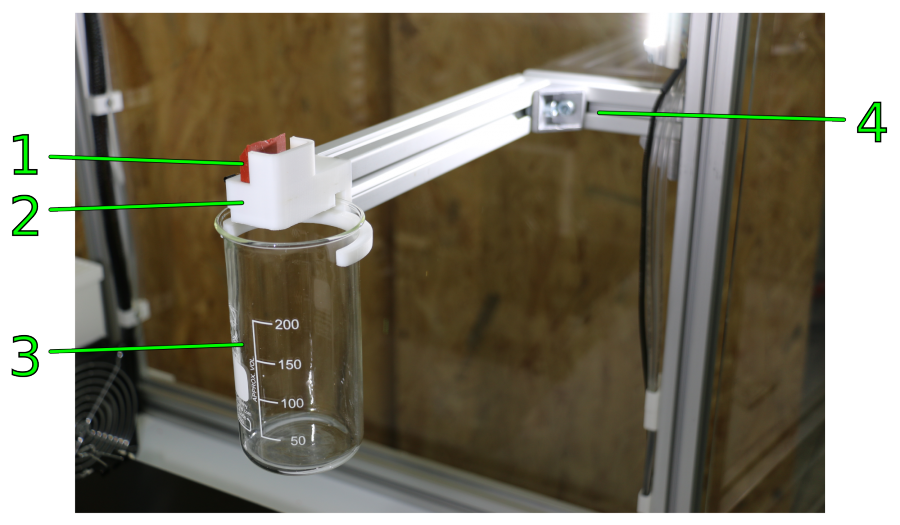
\includegraphics[width=.7\linewidth]{./img/desc_wiper.png}
  \caption{The wiper makes sure that the nozzle tip is always clean and well filled after a tool change during dual-material print jobs.}
\end{figure}

The HT500.3 3D Printer is equipped with a wiper to enable high-quality dual extruder printing.

During every tool change of a dual-extruder print, the nozzle to be used next will be primed and wiped to ensure pressure loss during its pause time is compensated and the nozzle starts well filled. 



\subsection{Electronic chamber}

\begin{figure}[H]
  \centering
  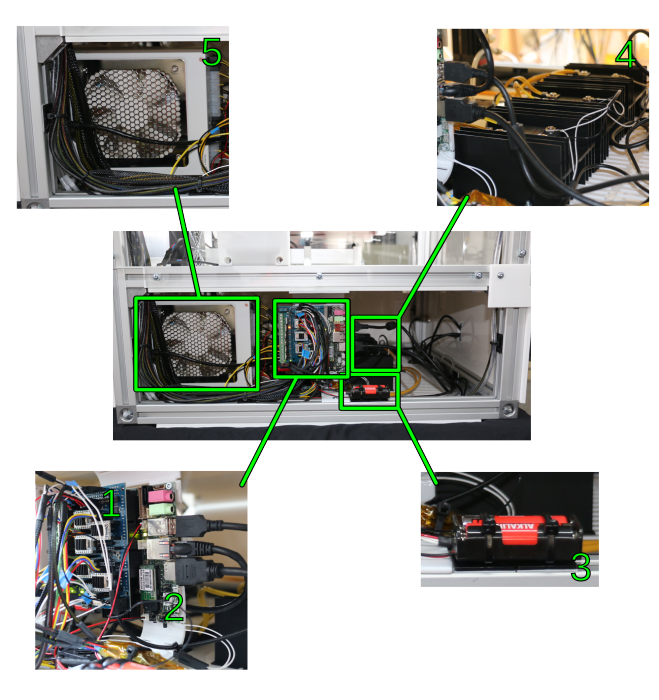
\includegraphics[width=.7\linewidth]{./img/desc_ht-500_overviewelectronicchamberleft.png}
  \caption{Inside view of the electronic chamber (left side).}
\end{figure}

\begin{table}[H]
  \centering
  \begin{tabulary}{\textwidth}{ L L }
    \toprule
    No.  &  Description \\
    \midrule  
    1    &  RADDS v1.5 3D Printer Driver Shield \\
    2    &  UDOO Quad Single Board Mini PC \\
    3    &  3V power supply for internal real-time clock \\
    4    &  Solid State Relays on cooling substructure \\
    \bottomrule
  \end{tabulary}
\end{table}

All control elements are installed in the electronic chamber together with the 12V(DC) mains adapter and the cooling unit.

The chamber is completely covered with white acrylic sheets fastened to the aluminum frame with hexagon socket screws and hammerhead nuts.

The RADDS 3D Printer Driver Shield in conjunction with the SAM3X microcontroller on the UDOO board controls all processes of the printing process, i.e. the drives, the heating resistors, heating fans and the temperature sensors.

The UDOO Quad Single Board Mini PC provides the GUI of the touchscreen and the ethernet connection and processes the G-codes of the slicing software.
Slots in the bottom cover provide an air inlet for the cooling unit.

When the 3D Printer is switched off the internal real-time clock of the Mini PC is fed by two external batteries so that the system's time signal is not lost.

The solid state relays switch the four heating resistors of the build chamber heating and the heating resistor of the print table.

\subsection{Cooling system}

The cooling unit consists of a pump with water reservoir, a radiator and the closed loop coolant circuit filled with an electronic cooling liquid. It is automatically switched on and off when the build chamber is activated/deactivated.

The coolant is pumped in a circle past the motors and the extruder nozzles where it absorbs heat which is then emitted via the radiator.

Check the coolant level monthly and if required, refill as described in the Service Guide. 

\begin{figure}[H]
  \centering
  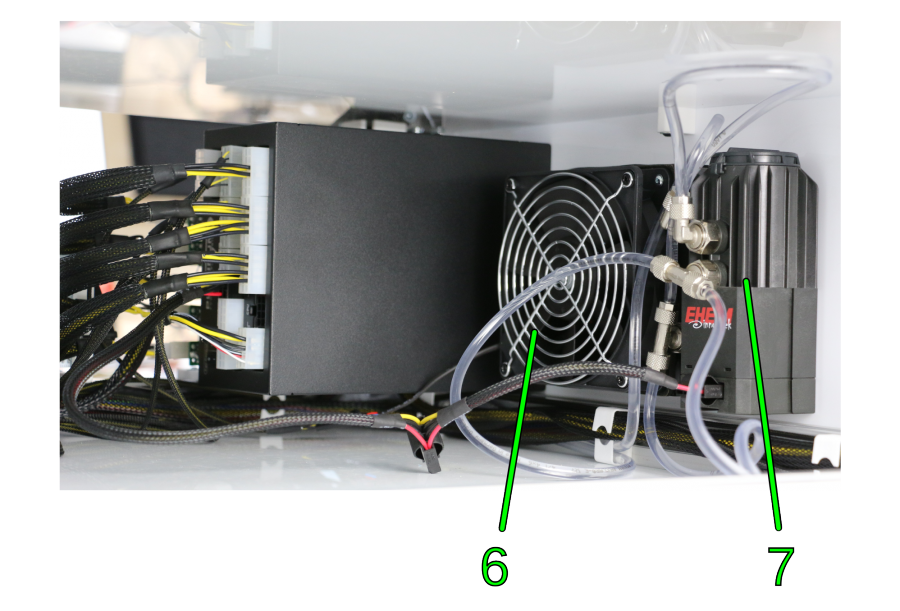
\includegraphics[width=.7\linewidth]{./img/desc_ht500_overviewelectronicchamberright.png}
  \caption{Inside view of the electronic chamber (right side).}
\end{figure}

\begin{table}[H]
  \centering
  \begin{tabulary}{\textwidth}{ L L }
    \toprule
    No.  &  Description \\
    \midrule  
    6    &  Cooling unit radiator \\
    7    &  Cooling unit pump \\
    \bottomrule
  \end{tabulary}
\end{table}

\subsection{Connections and Controls}

\begin{figure}[H]
  \centering
  \includegraphics[width=.7\linewidth]{./img/desc_overviewelectronicchamberhind_typeplate.png}
  \caption{Rear cover}
\end{figure}

\begin{table}[H]
  \centering
  \begin{tabulary}{\textwidth}{ L L }
    \toprule
    No.  &  Description \\
    \midrule
    8    &  Type plate \\
    9    &  Cooling unit water pump and radiator grill \\
    10   &  Mains plug \\
    11   &  Main switch \\ 
    12   &  RJ45 ethernet plug \\
    13   &  230V supply cable with Schuko plug \\
    \bottomrule
  \end{tabulary}
\end{table}

At the rear cover you find the mains plug and the main switch of the mains adapter and the RJ45 ethernet plug for the network connection.

The cooling systems' accumulated warmth is dissipated via the radiator grill to the outside.
The type plate is positioned next to the fixing screws of the cooling water pump. 

\begin{table}[H]
  \centering
  \begin{tabulary}{\textwidth}{ L L }
    \toprule
    No.  & 	Description \\
    \midrule
    14   &	10\textquotedbl TFT high-resolution touchscreen with Graphical User Interface (GUI) \\
    15   &	Wake button \\
    \bottomrule
  \end{tabulary}
\end{table}

\begin{figure}[H]
  \centering
  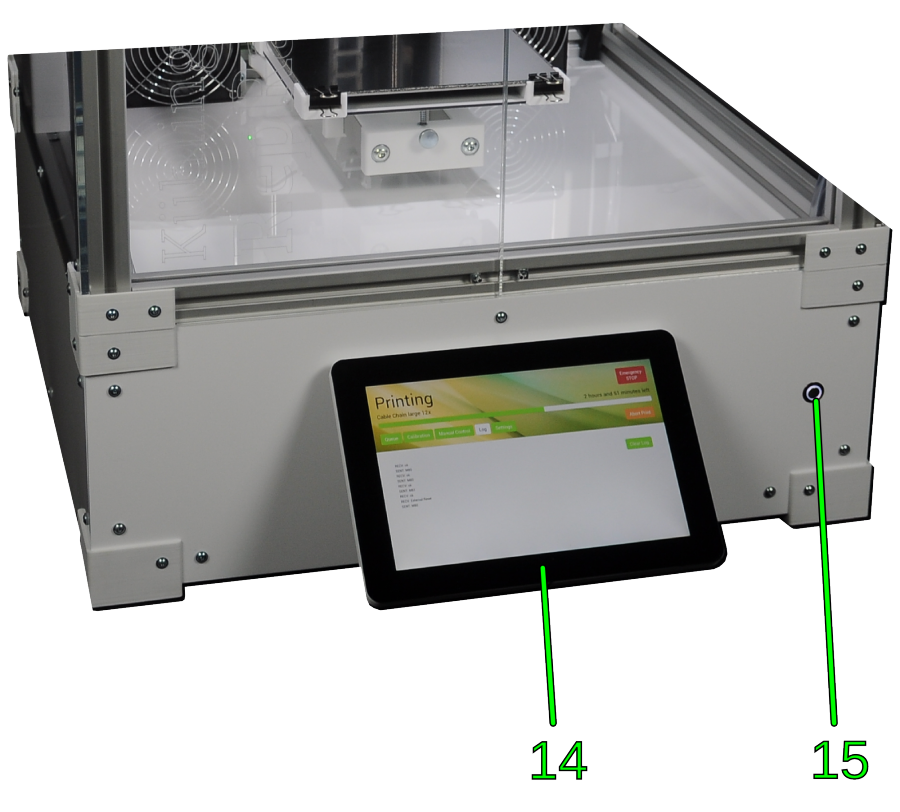
\includegraphics[width=.7\linewidth]{./img/desc_ht500_electronicchamberfront.png}
  \caption{Touchscreen user interface and wake button at the front cover}
\end{figure}

The wake button at the front panel provides a wake-up function and indicates the general operating status of the 3D Printer. It is equipped with a light ring that is illuminated while operational and dims after the 3D Printer has been shut down. Press the button to restart the 3D Printer from standby.

All 3D Printer operation is carried out via the Graphical User Interface at the touchscreen. 



\subsection{Touchscreen operation}

Operating the HT500.3 is designed to be comfortable and intuitive. Therefore, a high-resolution 10\textquotedbl TFT touchscreen mounted at the front panel provides an easy-to-use Graphical User Interface (GUI).

All operation of the HT500.3 is carried out via the RepRapOnRails operating software which provides status messages and control functions that can be chosen by simply tapping the respective buttons. Find detailed explanations of functions and operating procedures in the Operating Manual.

\begin{figure}[H]
  \centering
  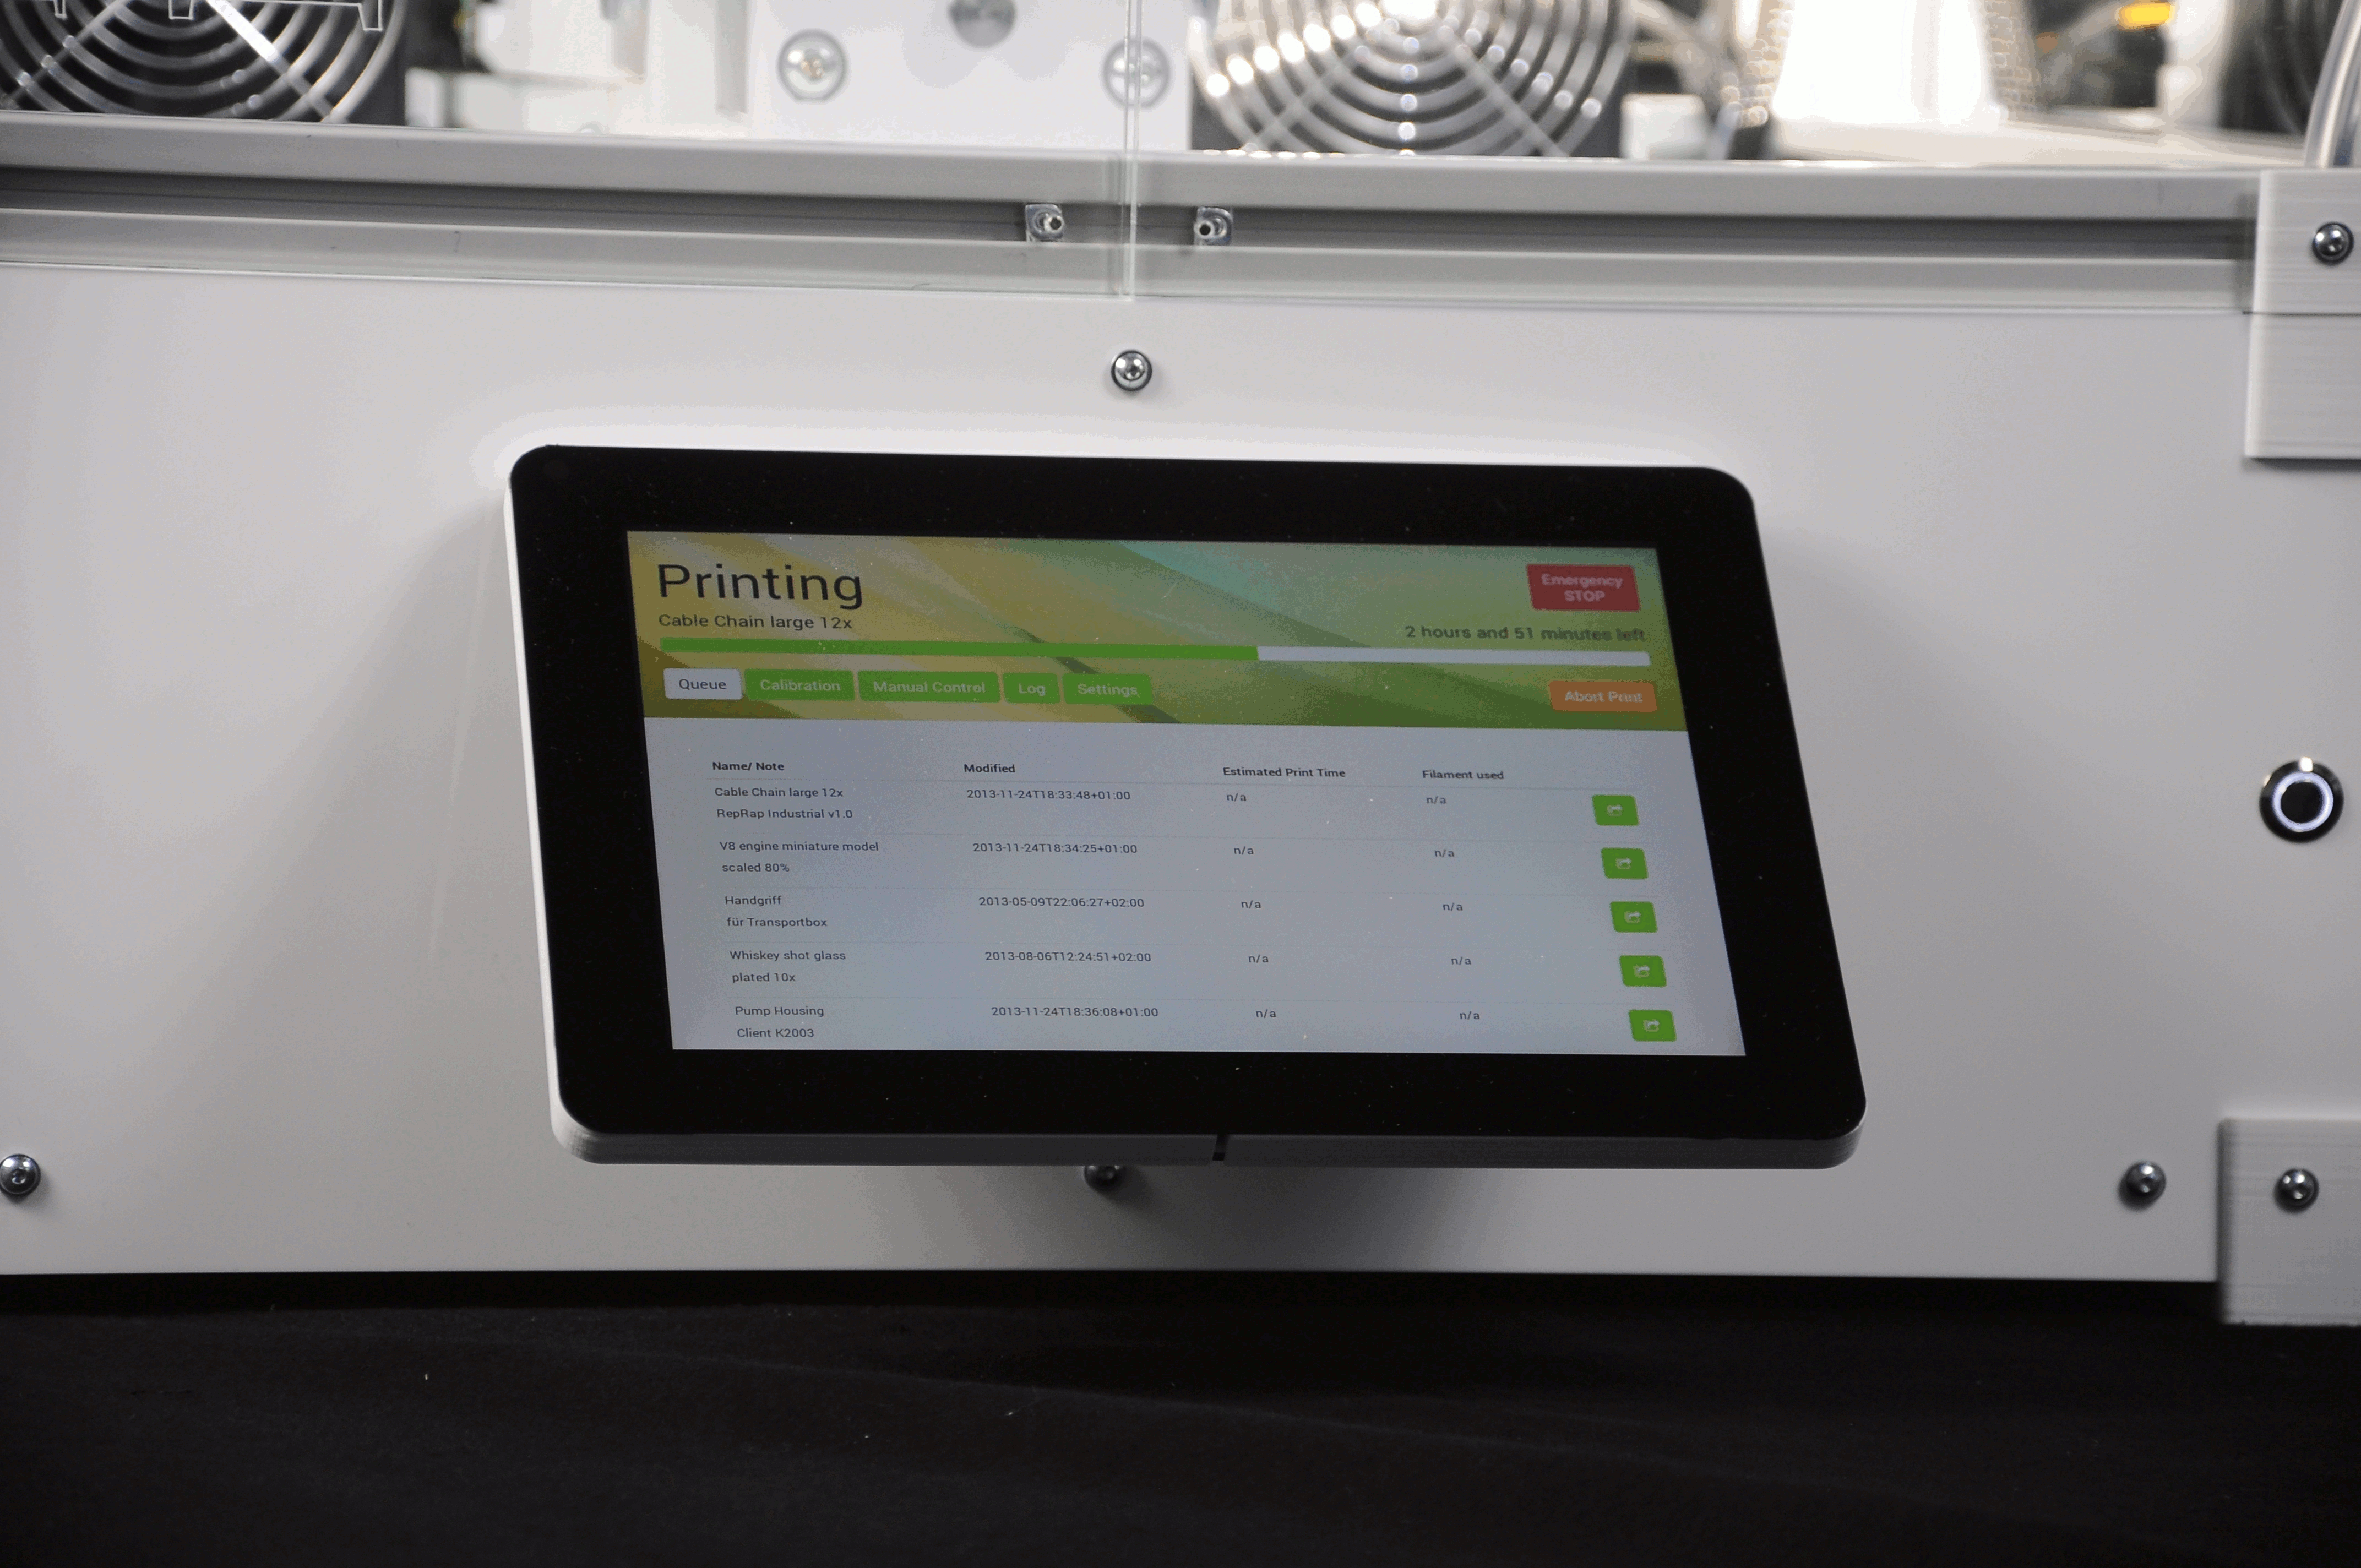
\includegraphics[width=.7\linewidth]{./img/touchscreen.png}
  \caption{The high-resolution 10\textquotedbl-TFT touchscreen mounted at the front panel enables direct operation of the HT500.3.}
\end{figure}

The currently installed version
of the operating software is displayed on the right-hand side of \emph{Setup} menu together with additional system information.

\begin{figure}[H]
  \centering
  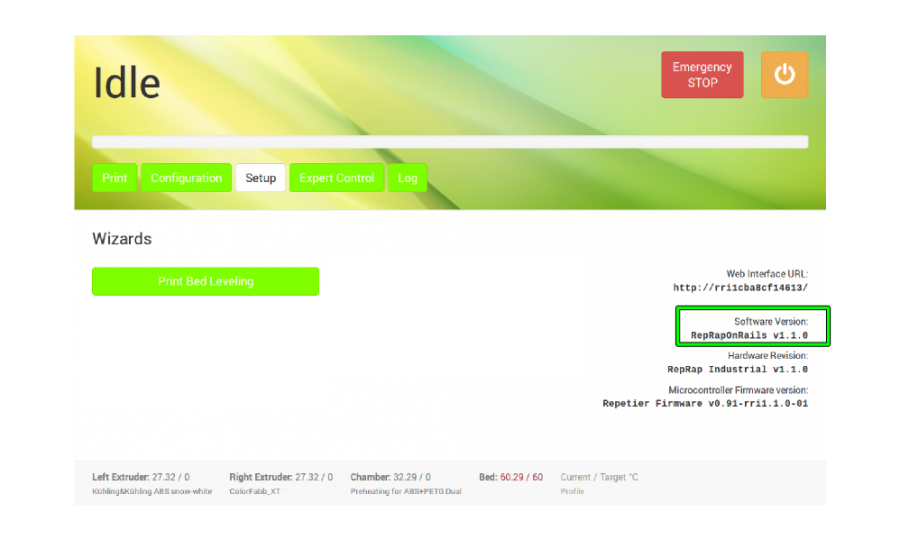
\includegraphics[width=.7\linewidth]{./img/gui_setupmenu_rrorversion.png}
  \caption{RepRapOnRails software version displayed in the \emph{Setup} menu.}
\end{figure}


\section{Transport and installation}



\subsection{Life cycle}

Find everything you need to know after you ordered your HT500.3 3D Printer in the following paragraphs. From the day of your invoice until the day you want to dispose of the apparatus and anything in between is explained here. 


\subsubsection{Delivery}

The HT500.3 3D Printer arrives at your place fully assembled and can be commissioned directly after setting it up and connecting the power supply.
The 3D Printer is delivered in a transport box on a palette. It is advisable to leave the HT500.3 packed and on the palette until moving it to its final installation site for commissioning.
At the installation site, unpack the HT500.3 according to the information in the accompanying Quick Start Guide.
Dispose of the packaging in accordance with the local waste disposal regulations.
After unpacking, inspect the apparatus for:

\begin{itemize}
  \item damage in transit
  \item completeness of the delivery (compare delivery note)
\end{itemize}

If you notice any deviants, please immediately inform the hauler and the manufacturer. \emph{Do not} put the HT500.3 to use with defective parts.


\subsubsection{Transport}

To avoid injuries and property damage observe the following notes when transporting the HT500.3:

\begin{itemize}
  \item The apparatus' weight exceeds 50 kg. Always carry it \emph{two by two}.
  \item Keep the HT500.3 horizontal to avoid damaging internal parts.
  \item Avert shock loads to the housing.
\end{itemize}


The HT500.3 has been designed for stationary application. It is not equipped with special transport devices such as lifting eyes or handles. The feet provide sufficient clearance to lift the apparatus and carry it to the installation site.
While the HT500.3 is packed and on its transport palette, use a lifting cart or pallet stacker for transportation. Make sure that the weight is evenly distributed and secure the HT500.3 against tilting. 

\begin{info}
  The housing is not designed for subsequently attaching lifting eyes. If you need to transport the 3D Printer longer ways, load and secure it on a stable pallet and transport it with a pallet stacker or lifting cart.
  Detailed information about safeguarding and packing the 3D Printer for shipping can be found in the Service Guide.
\end{info}


\subsubsection{Storage}

If the HT500.3 must be stored away, choose a leveled storage site and make sure that the 3D Printer does not stand on a ledge.
Before storing it, clean the HT500.3 and protect it from dust with a plastic tarpaulin or air cushion foil.

\begin{notice}
  Do not cover the 3D Printer with a textile sheet since the fibers may enter the supply system and clog the nozzles after recommissioning. Use lint-free plastic sheets only.
\end{notice}

The storage ambient conditions for the HT500.3 and its components are stated in the data sheet. For recommissioning after lengthy periods of storage follow the information given in initial commissioning. 


\subsubsection{Environment, recycling and disposal}

When used as intended, the HT500.3 presents no environmental danger.
However, the internal cooling works with a coolant that can be environmentally dangerous when leaking (see data sheet). Please observe the manufacturer's safety data sheet when handling the coolant.
The materials used for printing can also be environmentally dangerous when handled improperly. Always observe the manufacturer's safety data sheet and process plastics only within the limit values specified therein and with respect to the safety instructions.

\emph{Generally, consider the environment}: the auxiliary and operating materials of the HT500.3 can be dangerous to environment and health.
Awareness and foresighted behavior help avoiding ecological and personnel damage.
Components may bear valuable elements such as rare earths, or may be reusable. Do not waste them by inadequate and thoughtless disposal.
Environmentally hazardous substances \emph{must not} trickle into the soil or enter the sanitation. They must be stored in suitable containers and be disposed off adequately and in accordance with local and national regulations.

The HT500.3 is recyclable due to its low-pollution equipment. Nonetheless, the European Guideline 2002/96/EG (Waste Electrical and Electronic Equipment - WEEE) and the German \emph{Elektro- und Elektronikgesetz} (ElektroG) forbid the disposal of the apparatus via the household garbage. For environmental friendly recycling and disposal of the HT500.3 please contact a certified electronic waste management professional.

\begin{info}
  Kühling\&Kühling emphasize that there is no redemption obligation in this regard.
\end{info}



\subsection{Setup and Installation}

Use a lifting carriage to bring the HT500.3 on its transport pallet as near to its setup site as possible. Before setting up the HT500.3 remove the lid and side walls of the transport box and all straps. Subsequently, lift the apparatus off the transport pallet two-by-two and carefully carry it to its final installation location. 

\subsubsection{Installation requirements}

\begin{notice}
  The apparatus must not be set up in a surrounding with high formation of dust (e.g. near woodworks etc.). Ingress of particles into the filament supply system can lead to intense cleaning efforts due to clogging of the nozzles and thus immense non-productive time.
\end{notice}

Set up the HT500.3 at a well aerated place with an all-season ambient temperature between 15 and 25\degree C and a maximum relative humidity of 70\%.
Position the HT500.3 on a flat, carrying and enduring surface with a load capacity of at least 75 kg.
To ensure unhindered aeration of the electronic chamber no soft, movable materials (e.g. table cloth, cardboard strips, paper etc.) may be placed underneath the apparatus to prevent clogging of the vent slots.
The required setup space must at least be 650 x 650mm and provide approximately 500mm free space to either side to enable unhindered access to the electronic chamber for service and maintenance work. At least 750mm free space must be left at the back of the HT500.3 to make changing the material easy and to ensure free air circulation at the ventilation grill in the back cover. At the front a free space of 1.250mm is recommended to allow easy operation with open chamber doors.
To easily access the touchscreen in a sitting or standing position the height of the setup table should not undercut 780mm.
A 230V power source must be within the range of the connection cable. 


\subsubsection{Unpacking the machine}

\begin{figure}[H]
  \centering
  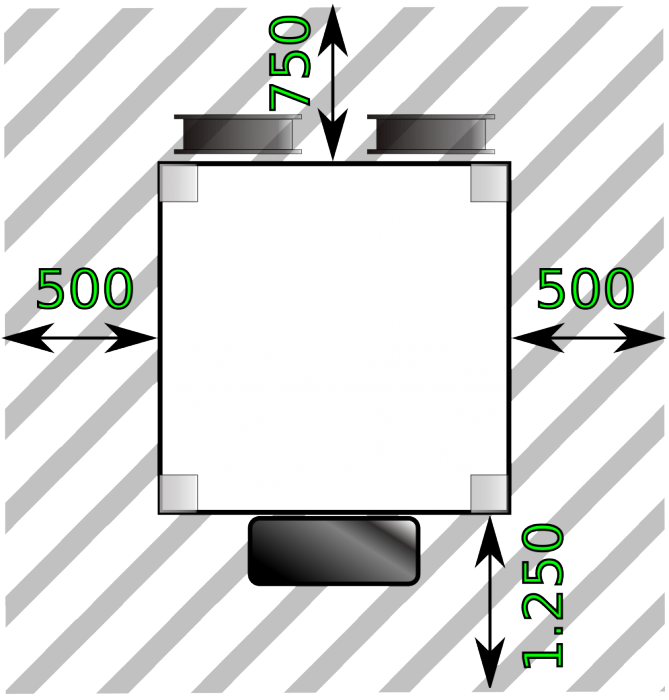
\includegraphics[width=.7\linewidth]{./img/workspace.png}
  \caption{Necessary free space around the HT500.3}
\end{figure}

\begin{danger}
  OF CUTTING INJURIES AND EYE DAMAGE\\
  The packing straps are pretensioned and may whip when cut, causing cutting injuries or eye damage.
  \begin{itemize}
    \item Hold down the top part of the strap and cut it at the side. Make sure it does not hit somebodies face.
  \end{itemize}
\end{danger}

\begin{danger}
  OF CUTTING INJURIES\\
  The transport box is made of unfinished plywood and may hold splinters and sharp edges that can cause cutting injuries.
  \begin{itemize}
    \item Take care when removing the transport packaging and wear protective gloves.
  \end{itemize}
\end{danger}

\begin{notice}
  If the 3D Printer has a temperature below 16\degree C (e.g. directly after delivery in cold weather) there is a danger of air humidity condensing on sensitive electronic components. This can lead to severe damages due to short circuiting during commissioning.
  Therefore, it is necessary to thoroughly let the 3D Printer warm up to ambient temperature for at least 12 hrs. at its operating place 
  \emph{prior} to commissioning.
  Regard the ambient conditions required for operation.  
\end{notice}

To unpack the machine, cut the tensioning straps of the transport box, remove the lid and carefully lift the box over the printer.
Then cut the tensioning straps around the 3D Printer and remove the wooden cover plate and the air cushion foil.
Set aside and store all parts of the transport packaging for later use, e.g. moving or shipping the 3D Printer. 

\begin{figure}[H]
  \centering
  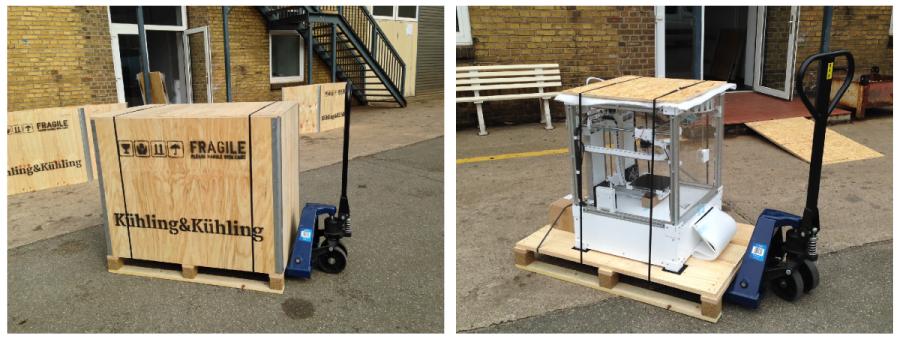
\includegraphics[width=.7\linewidth]{./img/secure_boxed.png}
  \caption{The box and the lid are fastened to the pallet with tensioning straps.
           The 3D Printer is padded with air cushion foil and a wooden cover plate and strapped to the pallet with tensioning straps.}
\end{figure}

\begin{info}
  Find detailed information on repacking the machine for shipping in the Service Guide.
\end{info}


\subsubsection{Removing the transport restraints}

All moving components of the HT500.3 3D Printer are secured with blue tape against damage in transit.
Make sure all transport restraints named in the adjacent pictures have been removed before commissioning the 3D Printer.

\begin{figure}[H]
  \centering
  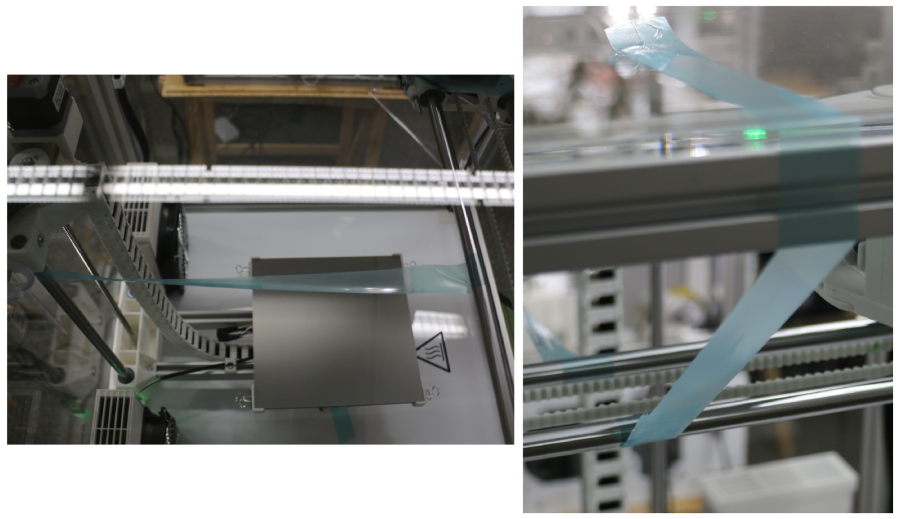
\includegraphics[width=.7\linewidth]{./img/secure_yaxis.png}
  \caption{Transport restraint of the Y-axis: blue tape spans from the hind Y-shaft to the left Z-shaft and from the front Y-shaft to the top 
           cover.}
\end{figure}

\begin{figure}[H]
  \centering
  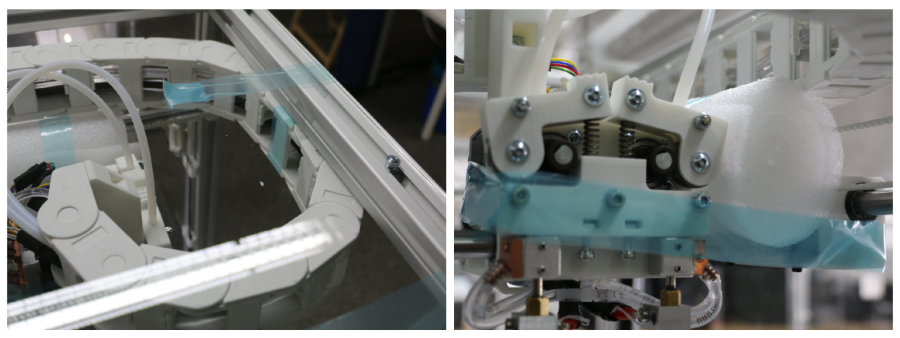
\includegraphics[width=.7\linewidth]{./img/secure_headchain.png}
  \caption{Transport restraint of the main e-chain: blue tape is strapped around the chain an fastened to the top cover.
           Transport restraint of the extruder head: the extruder head is cushioned with air cushion foil and strapped to the 
           right X-end with blue tape.}
\end{figure}

\begin{figure}[H]
  \centering
  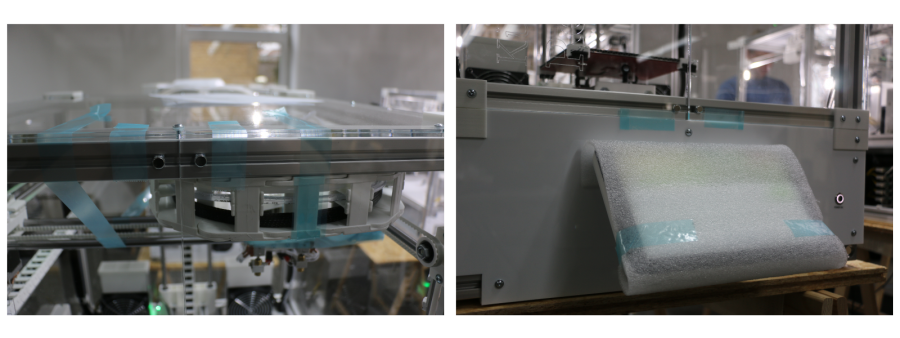
\includegraphics[width=.7\linewidth]{./img/secure_doors.png}
  \caption{The doors are held close by blue tape at the top and lower edge.
           The touchscreen is packed in air cushion foil.}
\end{figure}

\begin{figure}[H]
  \centering
  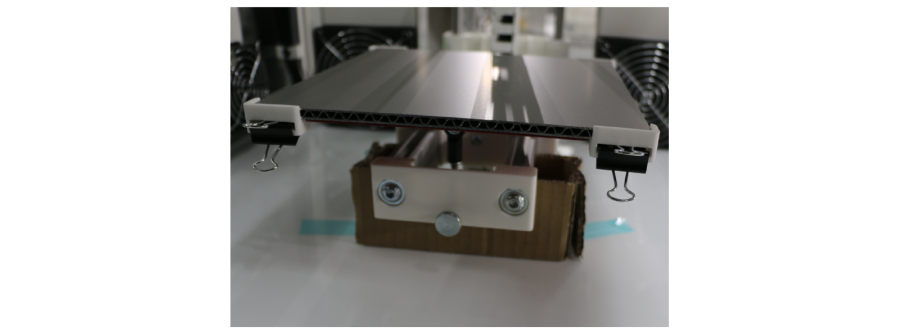
\includegraphics[width=.7\linewidth]{./img/secure_table.png}
  \caption{A cardboard frame supports the print table.}
\end{figure}


\subsubsection{Connections}

After setting the apparatus up it must be connected to the power supply and the data network.

\begin{enumerate}
  \item Set the power supply main switch at the back of the 3D Printer to \emph{<0>} (OFF).
  \item Unpack the supply cable and connect it to the mains plug at the backside.
  \item Connect the Schuko plug to a 230 V socket.
  \item Connect the HT500.3 to your data network by plugging the network cable into the RJ45 ethernet plug. 
        Your network must provide DHCP IP address management and should be connected to the internet (to enable the printer to fetch current time signal via Network Time Protocol (ntp)).
\end{enumerate}

\subsubsection{Initial commissioning}

After set-up has been completed the further commissioning of the HT500.3 takes place at the web interface and the touchscreen as described in the Operating Manual. 

\subsection{Decommissioning}

Decommissioning may be necessary on two occasions: the temporary decommissioning if the 3D Printer will just be out of operation for a limited time (e.g. moving) or the permanent decommissioning if the 3D Printer has expired its lifetime and will be scrapped.


\subsubsection{Temporary decommissioning}

 If you need to take the HT500.3 out of operation to move or store it, regard the following information:
\begin{itemize}
  \item Remove remaining filament from the supply system.
  \item Clean the 3D Printer, especially the extruder nozzles.
  \item Move all axes into their home positions.
  \item Disconnect the mains cable and the network cable. Store them together with the 3D Printer 
        (e.g. fixed with adhesive tape inside the build chamber).
  \item Protect the print table surface and the touchscreen with a cardboard pad against scratching.
  \item Secure the extruder head, the print table, and the build chamber doors with strapping tape tape against moving (see Transport).
  \item Position the 3D Printer on a transport pallet and cover it with a plastic tarpaulin or air cushion foil.
\end{itemize}

\begin{notice}
  Do not cover the 3D Printer with a textile sheet since the fibers may enter the supply system and clog the nozzles after recommissioning. Use lint-free plastic sheets only.
\end{notice}

\begin{itemize}
  \item Use lashing straps to secure the 3D Printer on the transport pallet. 
\end{itemize}


\subsubsection{Permanent decommissioning}

 If you do not want to use the HT500.3 any longer or if it is damaged beyond repair:
\begin{itemize}
  \item Take the HT500.3 out of operation as described above.
  \item Drain the cooling system and collect the coolant. 
        Dispose of the coolant according to your local guidelines and the manufacturer's data sheet.
  \item Disassemble all components according to their recyclablility and dispose of them adequately and lawfully.
\end{itemize}

\begin{info}
  Components may bear valuable elements such as rare earths, or may be reusable. Do not waste them by inadequate and thoughtless disposal.
\end{info}



\subsection{On demand maintenance}

The HT500.3 3D Printer features a low-maintenance design, thus intensive maintenance time is not required during normal operation. Nonetheless regard the maintenance intervals stated in the Service Guide.

Apart from this, regular cleaning will mostly suffice to keep your 3D Printer running satisfactorily.


\section{Initial commissioning}

After the installation the HT500.3 is ready for initial commissioning. The first few steps will prepare your HT500.3 for its day-to-day duty:

\begin{itemize}
  \item Make sure that no foreign objects are left in the build chamber 
        (transport locks, tools or the like).
  \item Close the build chamber.
  \item Toggle the main switch to <I> (ON).
        When the power supply is switched on the 3D Printer will boot automatically. Please wait patiently until the full operating screen is loaded on the touchscreen at the machine front. The screen displays the Print screen and the top-left status message reads Idle.
  \item Tap [Build Chamber ON] in the [Print] screen of the user interface. The Build chamber lights will switch on, heater fans
        spin up and the axes will issue a reference movement to calibrate their home positions.
\end{itemize}


\subsection{Loading material}

First, material for the following print jobs must be provided:

\begin{itemize}
  \item Go to the [Expert Control] screen and tap [Maintenance Position] to move the print head to a middle front 
        position for convenient handling.
  \item Load the \emph{left extruder} with Kühling\&Kühling ABS material included 
        in the delivery for the first print.        
  \item Install the filament spool onto the corresponding spool carrier like shown in the description of the filament supply, section \ref{sec:filamentsupply}
  \begin{info}
    For installing other than the 750g spools delivered, adjusting the spool carriers may be necessary.
    The filament and chamber/bed profiles have been preset during factory test and are ready for use. For later changing the profiles refer to Configuration.
  \end{info}        
  \item Feed the end of the filament strand into the filament supply unit from below (passing through the cleaning sponge) 
        until it reaches the print head through its PTFE tube.
  \item At the print head, pull the PTFE tube out of the idler lever so you can grab the filament. Insert the filament through
        the idler lever from the top. Open a gap between the extruder drive gear and the idler bearing by pushing the lever down.
        Push the filament further down, passing the drive gear and entering the nozzle bore below.
  \item Slide the PTFE tube back into the idler lever so it is seated in there.
  \item In the [Configuration] screen select the corresponding filament profile with a suitable melting temperature for your material.
  \item Go to the [Expert Control] screen, select the extruder you have just loaded, check the suggested temperature
        and tap [SET] in order to preheat the print head. As soon as the target temperature is reached in the nozzle, buttons for
        [extrude] and [retract] are activated.
  \item When preheated, use [extrude] to successively push material through the print head. Each tap will forward the filament
        by 5mm. As soon as you see a consistent flow of molten plastic out of the nozzle, loading is finished.
  \item Switch of the nozzle heater by tapping [OFF].
  \item Repeat these steps for loading the right extruder if required.
\end{itemize}


\subsection{Preheating}

After material has been loaded and the hot-ends have been primed the next step is preheating the build chamber and the print bed in order to enable calibration at operating temperature: 


\begin{itemize}
  \item Check if the footer reads \emph{Preheating for ABS} for the \emph{Bed/Chamber} 
        profile. The footer is the same on every page of the GUI.
  \item If not switched on yet, activate the build chamber by tapping [Build Chamber ON]. The LEDs light up, the 
        fans start running and all axes perform a home-positioning routine.
  \item Then start the heating by tapping [Preheat Chamber/Bed ON]. The temperature 
        indicators in the footer now show both current and target temperature.
  \item Let the build chamber heat for \emph{approximately 45 minutes} until the target 
        temperature is reached.
\end{itemize}


\begin{figure}[H]
  \centering
  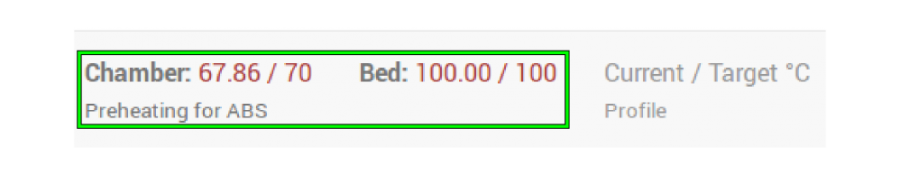
\includegraphics[width=.7\linewidth]{./img/gui_footercut_v110.png}
  \caption{Display of the selected chamber/bed profile in the footer.}
\end{figure}


\subsection{Calibration}

\subsubsection{Leveling the print bed}

When the target temperature is reached and stable level the print bed \emph{in the given order} to ensure that the hot-end nozzle tips have the same distance to the print bed at every point.

\begin{enumerate}
  \item Tap [Setup] to change to the Setup screen.
  \item Tap [Print Bed Leveling] to start the wizard that will guide you through the 
        leveling process.
  \item The wizard provides all necessary instructions on-screen. Read them thoroughly 
        and follow them step by step.
\end{enumerate}

\subsubsection{Determining the extrusion multiplier}

The “extrusion multiplier” allows for compensation of varying filament properties, first of all the cutting depths of the drive gear into the filament but also deviations of the diameter (also see Slic3r manual and Tips \& Tricks). The extrusion properties of any material, although chemically exactly the same, may differ from one filament spool to the other so that it is impossible to determine the correct extrusion multiplier prior to delivery. After leveling the print bed, it is therefore advised to calibrate the extrusion to adapt your printer to the installed filament in order to ensure a correct printing performance. 

To calibrate the extrusion, refer to the description in the Knowledge Base section of this manual.

\subsection{Creating your first print job}

You will find all necessary installation and setup procedures required for the first print in the following paragraphs. All software mentioned additionally is available “Open Source”. 

\begin{info}
  Kühling\&Kühling recommend using the stated software. Using other software is up to the user but the manufacturer cannot be held liable for any malfunction resulting from use of other than the recommended software.
\end{info}

\subsubsection{Installation and setup of the slicing software}

First you need to install a slicing software on your computer to 
translate .stl-files (Surface Teselation Language - a 3D format with triangulated surfaces needed for processing) into printable G-codes.

\emph{Kühling\&Kühling} recommend using the \emph{Slic3r Prusa Edition} slicing software to prepare your digital 3D models for printing. This slicing software provides a lot of features necessary for achieving optimal results with the HT500.3 and has been thoroughly tested. Other software may be available but has not been tested.

\begin{figure}[H]
  \centering
  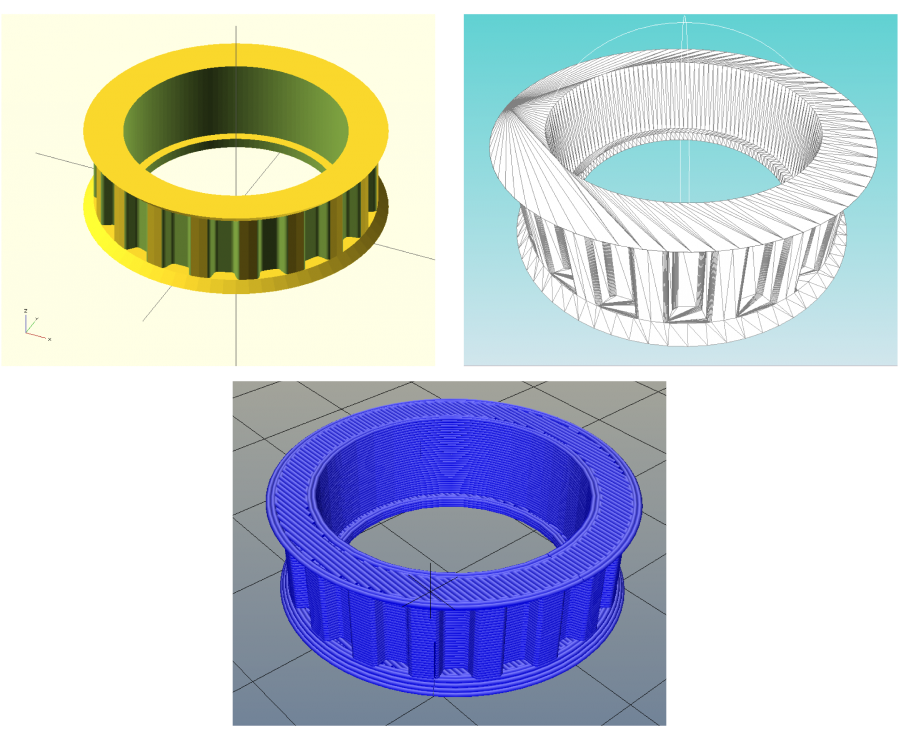
\includegraphics[width=.7\linewidth]{./img/opm_pulleyscadandsliced.png}
  \caption{A 3D model in its states during preparation for 3D printing: top-left - the 
           model preview in the 3D modeling software (view taken with OpenSCAD), top-right - the triangulated mesh after .stl-export (view taken with MeshLab), bottom-middle - the G-code preview after slicing shows the single layers calculated by the slicing software.}

\end{figure}

 To prepare for printing follow these steps:

\begin{enumerate}
  \item Download the latest Slic3r installation package for your operating. Links are referenced in the 
        Downloads section of this manual.
  \item Download the latest preconfigured Slic3r profiles package for the HT500.3 to a prepared directory on
        your PC, and unpack the archive. Links are referenced in the 
        Downloads section of this manual.
  \item In Slic3r select \emph{File > Load Config Bundle} and choose the previously downloaded 
        .ini file. Refer to the provided README.txt for a description of the different profiles available.
\end{enumerate}

\begin{figure}[H]
  \centering
  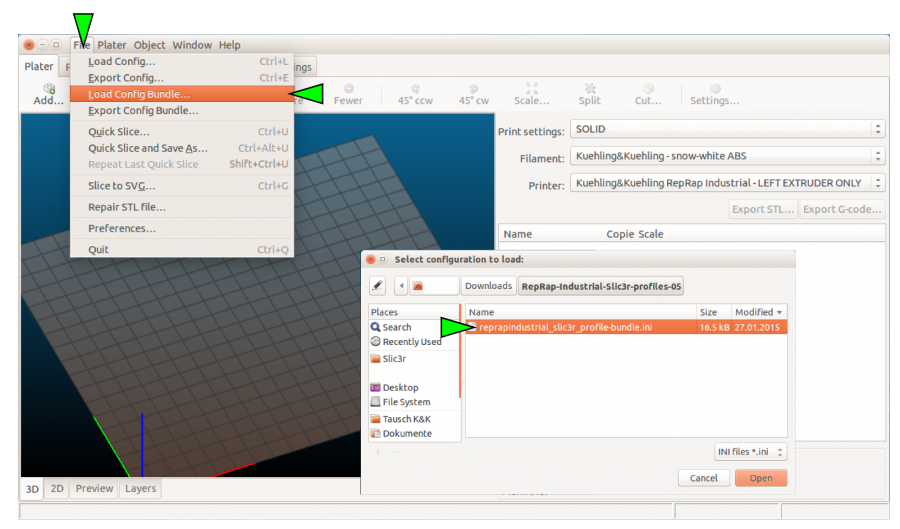
\includegraphics[width=.7\linewidth]{./img/slic3r_selectconigbundle.png}
  \caption{After importing the profile bundles Slic3r is equipped with all necessary 
           presets and ready for operation with the HT500.3 3D Printer.}
\end{figure}

\begin{info}
  When importing profile bundles into Slic3r, existing presets may be overwritten. It is recommended to backup your custom/modified presets by exporting them as a bundle first (File > Export Config Bundle).
\end{info}


\subsubsection{Slicing the 3D model}

The 3D model you want to print must be available as an \emph{.stl-file}. Most common 3D modeling software is able to create this file format.
\begin{enumerate}
  \item Start Slic3r to process a 3D model into G-code data.
  \item Select the preconfigured profiles for filament, print and printer before 
        generating a G-code file.
    \begin{itemize}
      \item Open the \emph{Filament Settings} tab end enter the extrusion multiplier measured during calibration.
      \item \emph{Rename and save} the filament profile.
    \end{itemize}
  \item Export the G-code data.
        Refer to the Slic3r manual for help on fine tuning any parameters for the printing process.
\end{enumerate}

\begin{figure}[H]
  \centering
  \includegraphics[width=.7\linewidth]{./img/slic3r_start_plater_select.png}
  \caption{Slic3r steps while crating a print job, including setting the extrusion 
           multiplier.}
\end{figure}


\subsubsection{Starting the print job}

Upload the GCODE to the 3D Printer via the web interface as described in Queue.

Make sure that all previously described steps have been carried out.
The next steps are carried out at the 3D Printer's GUI:
\begin{itemize}
  \item Tap the [print] button on the Print screen to start the print job.
  \item Wait until the apparatus has finished the print job completely and all axes are 
        in their home position, then remove the print bed, take off the test object and check whether all expectations have been met.
\end{itemize}

If everything has been fault-free, delete the print job from the queue - you are ready to proceed to production.

\begin{figure}[H]
  \centering
  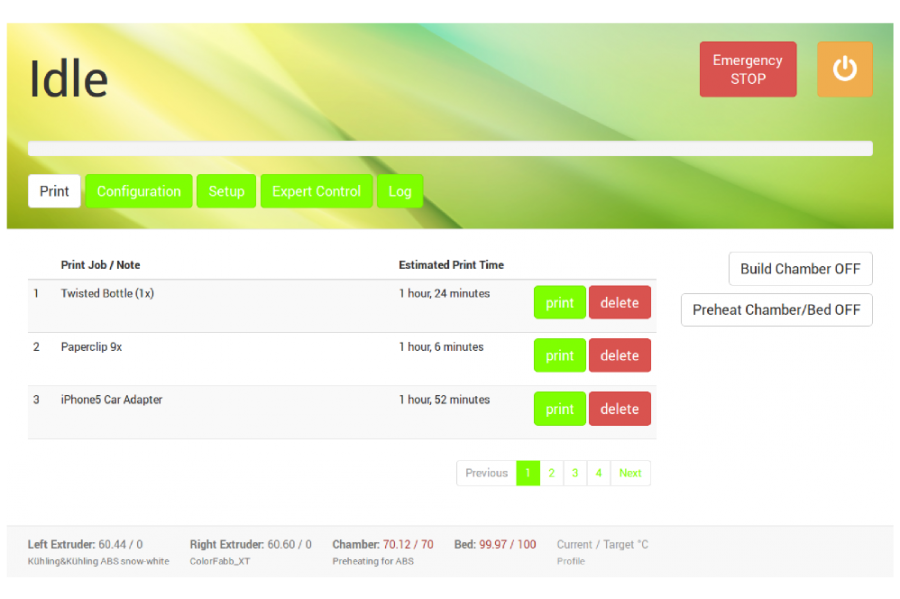
\includegraphics[width=.7\linewidth]{./img/gui_printtab_v110.png}
  \caption{GUI - “Print” selection menu}
\end{figure}

\subsubsection{Removing objects from the bed}

\begin{danger}
  By default the print bed and the build chamber heating resistors are not being switched off after a print job. Also, the extruder nozzles may still be too hot to the touch. Be careful not to burn yourself when removing the print bed
\end{danger}

\begin{notice}
  To avoid scratching do not use pointed tools (e.g. screwdrivers) to remove the object from the print bed.
  If residues of the print material remain on the print bed, use a very sharp, flat mounted blade to scrape the surface clean.
  Scratches in the print bed's surface may lead to enforced adhesion of prints. Severely scratched or broken print beds can no longer be used for production and must be replaced. 
\end{notice}

To remove printed objects from the print bed let the entire print cool down to room temperature; larger prints should remain in the switched off build chamber until cooled down.
With materials suited to being printed on PEI (e.g. ABS, HIPS, TPE-u) the print will loosen itself from the print bed when cooling due to shrinkage which can be heard by crackling noises. If otherwise, twist and bend the print bed until the object comes free. Breaking and even buckling the print bed is near impossible with manual force.
Other material-subsurface combinations may require some force or solving of the coating, rinsing the print bed with water for example is suitable when printing on PVA-glue.

Find more information about the properties and handling of the PEI print bed in the parts description of the Manual.


 
\section{Operation}

\begin{figure}[H]
  \centering
  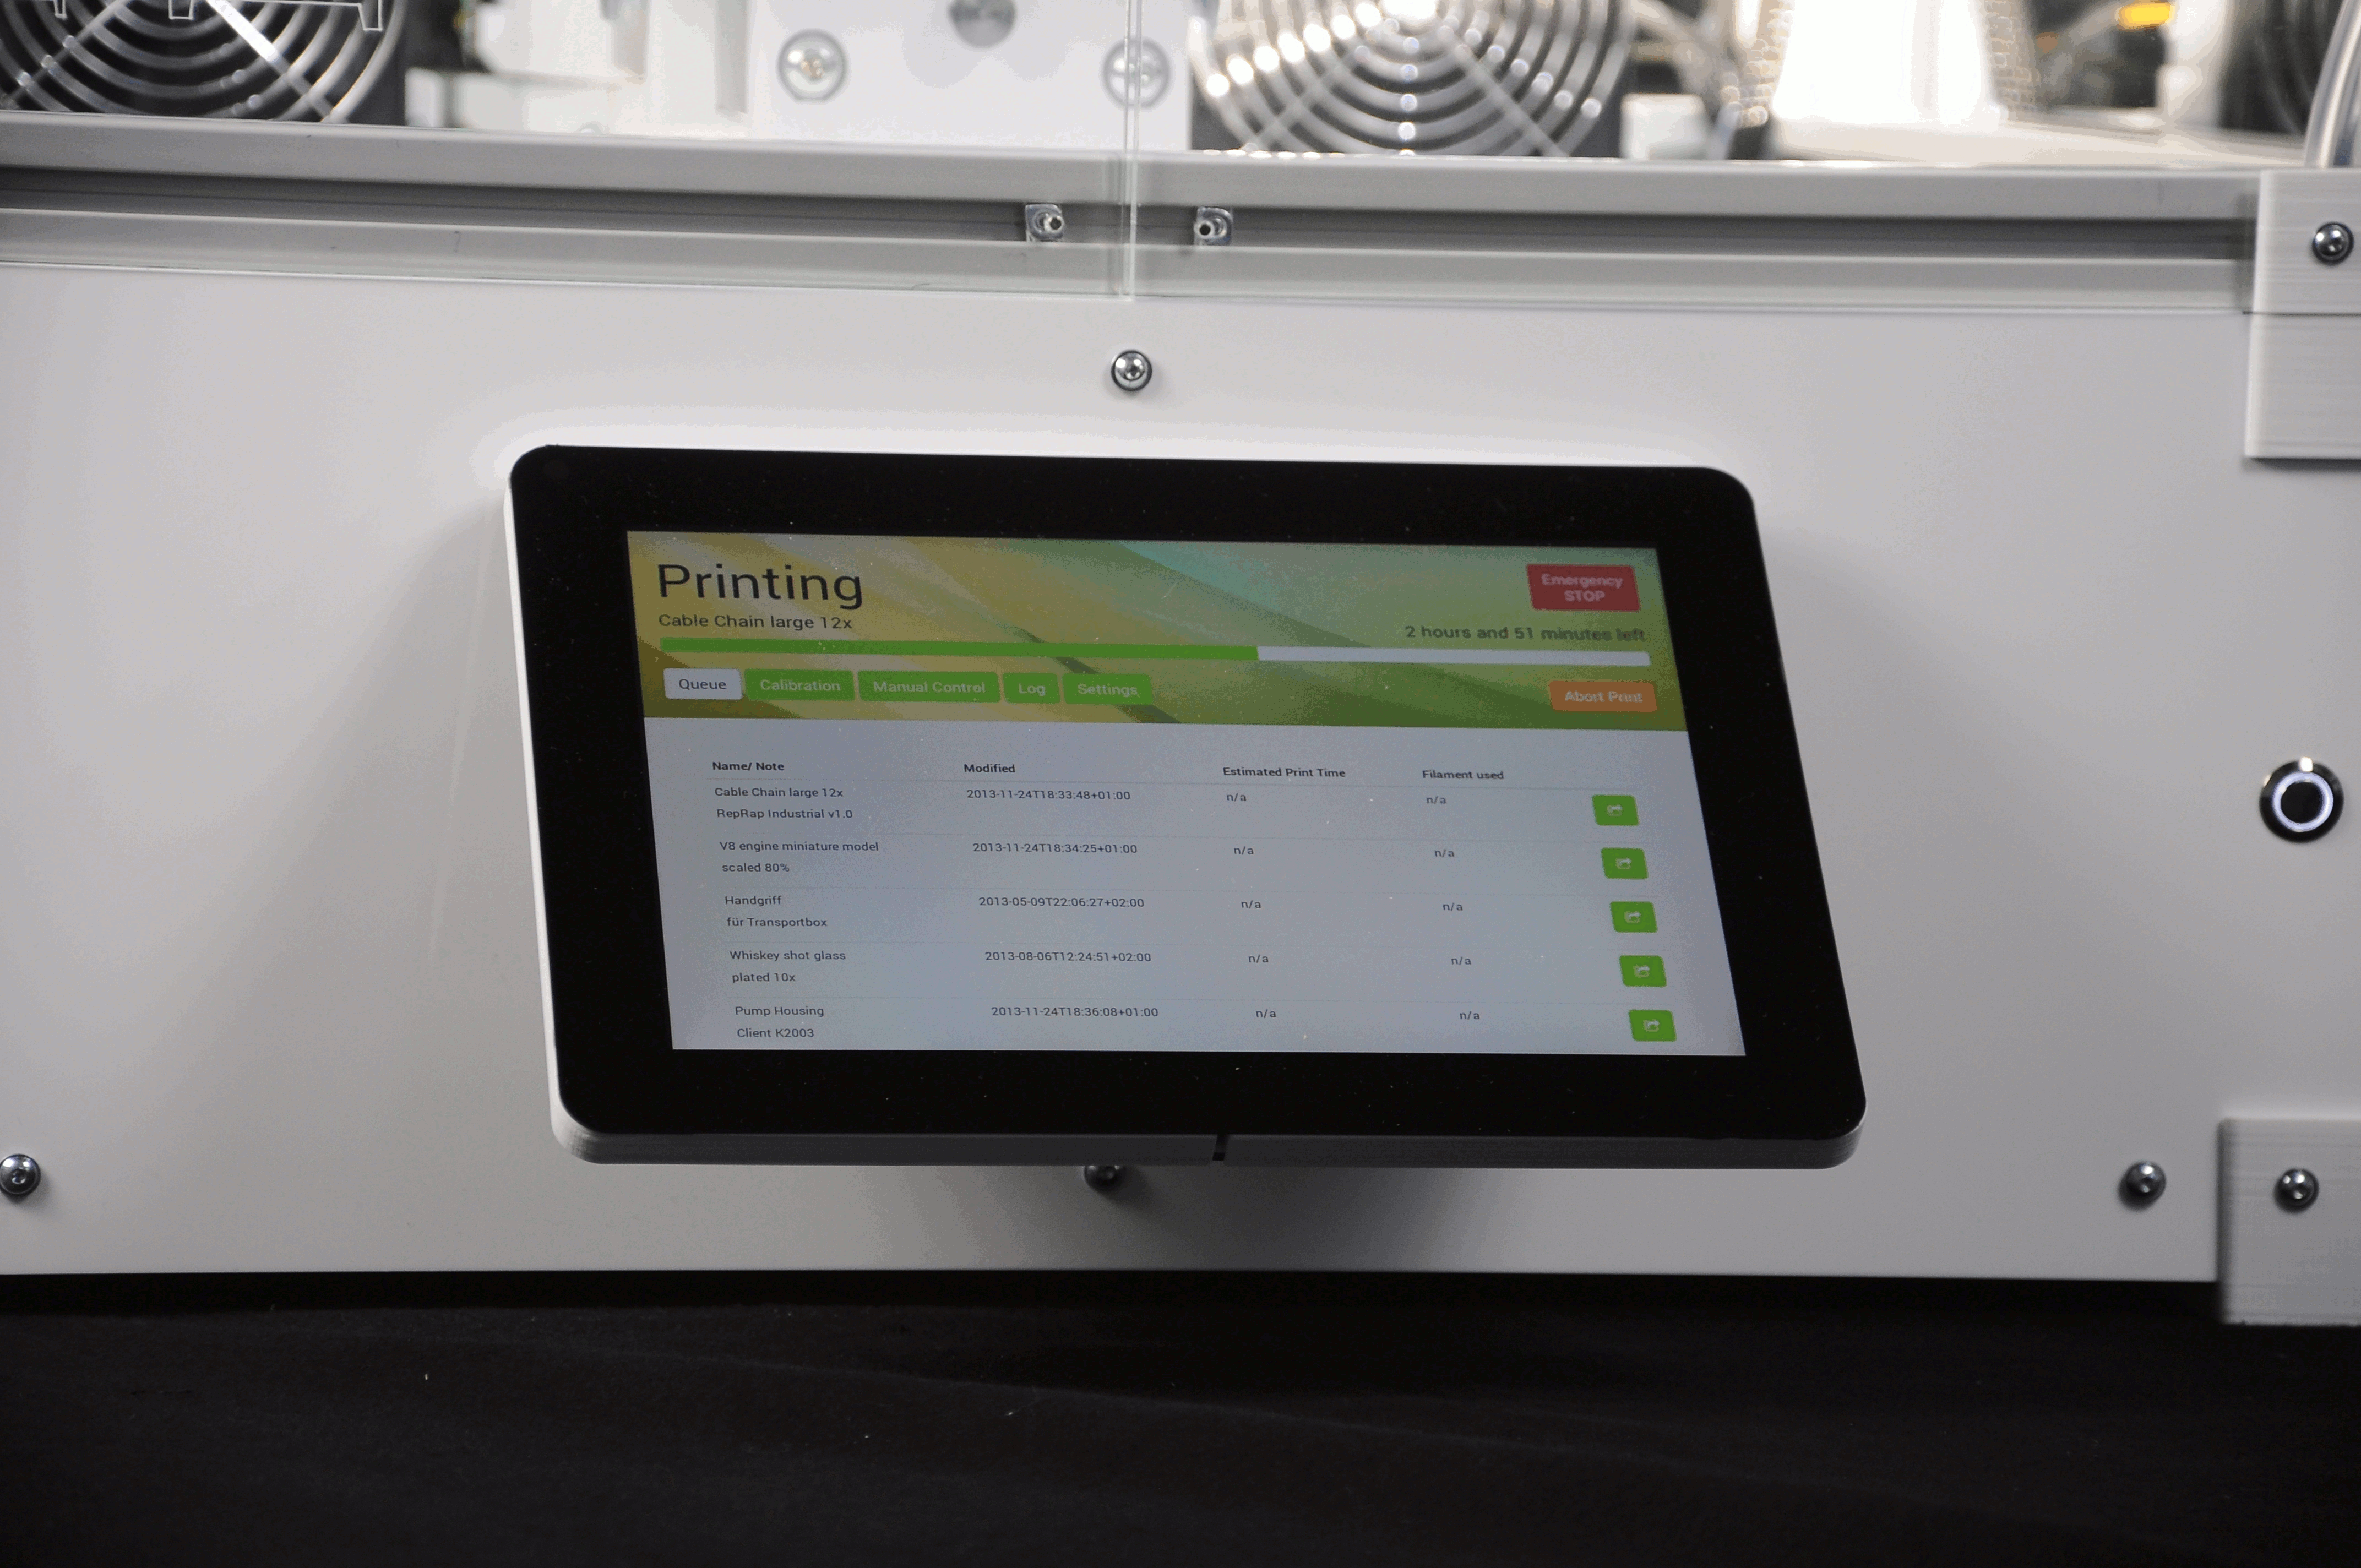
\includegraphics[width=.7\linewidth]{./img/touchscreen.png}
  \caption{The high-resolution 10\textquotedbl -TFT touchscreen mounted at the front 
           panel enables direct operation of the HT500.3.}
\end{figure}


This manual describes the initial commissioning of the 3D Printer after installation, the operation via the RepRapOnRails operating software and the all manual operating tasks that must be performed during normal day-today use.

\subsection{Starting the 3D Printer}

There are two possible states from which to start the 3D Printer: “switched off” and in “standby”. Either way starting the 3D Printer is a one-button-only procedure. After the boot sequence the operating screen starts with the Print screen in IDLE mode. 


\subsubsection{Switching on}

If the 3D Printer is switched off via the main switch at the rear cover 
(position \emph{<0>)} toggle the switch to \emph{<I>} (ON).
The 3D Printer will boot automatically.
It may take a few minutes until the touchscreen has fully loaded the operating screen - wait patiently without interfering.
The first screen will be the \emph{Print} screen with the (empty) print-job queue and the top-left status message displaying \emph{Idle}. 

\begin{figure}[H]
  \centering
  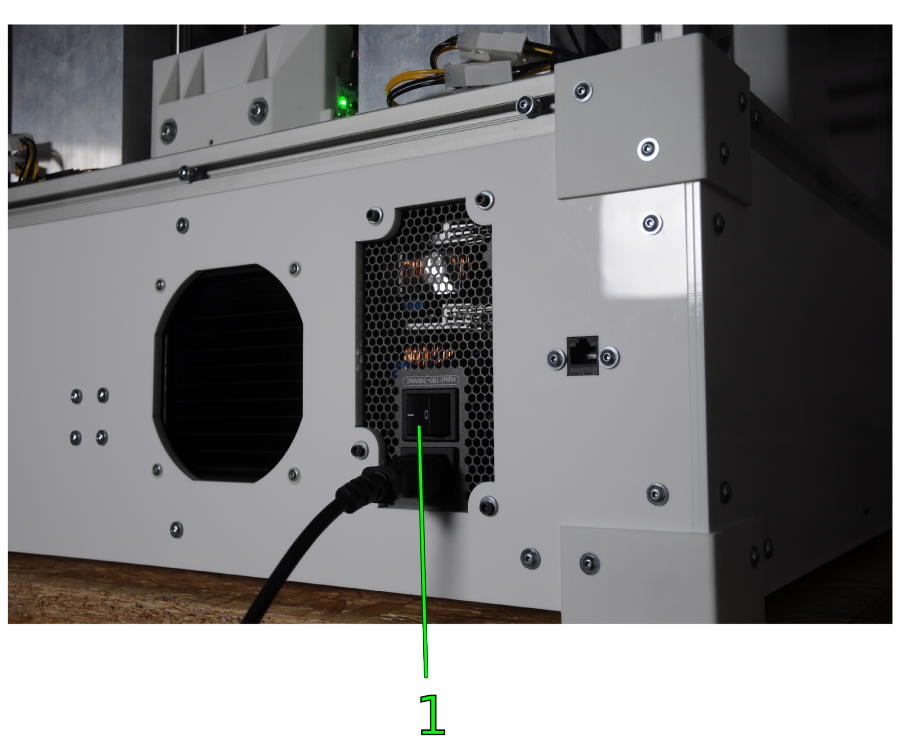
\includegraphics[width=.7\linewidth]{./img/opm_powerbutton.png}
  \caption{Powering up the 3D Printer.}
\end{figure}


\subsubsection{Waking from standby}

If the 3D Printer has been shut down via the touchscreen and set into standby mode (see section Print screen), press the wake button at the front cover. The light ring of the button lights up and the 3D Printer boots automatically.

\begin{figure}[H]
  \centering
  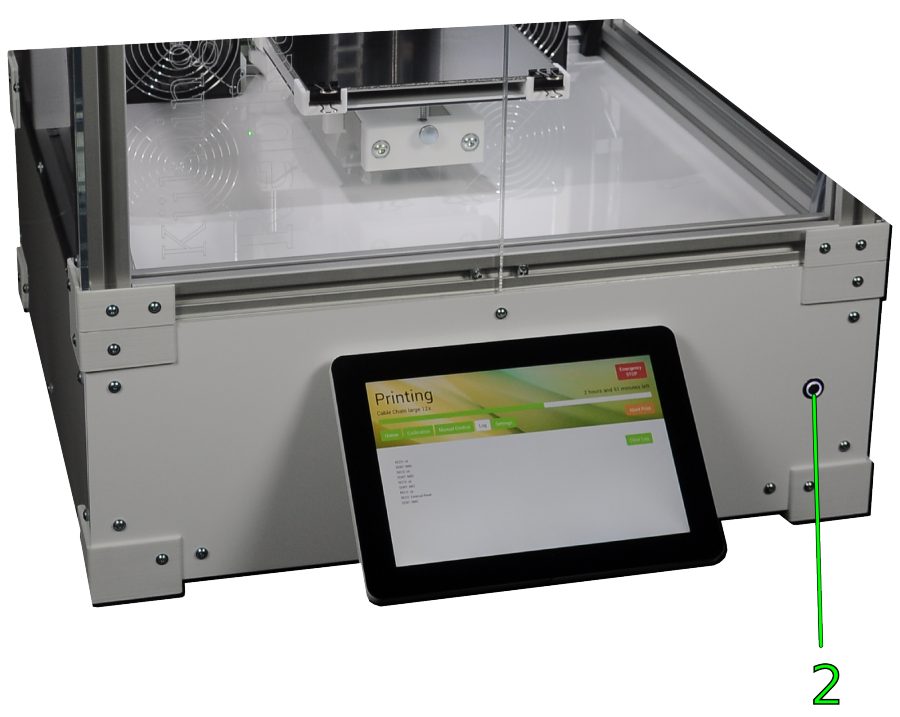
\includegraphics[width=.7\linewidth]{./img/opm_wakebutton.png}
  \caption{Waking the 3D Printer from standby.}
\end{figure}


\subsection{Graphical User Interface (GUI)}

\begin{figure}[H]
  \centering
  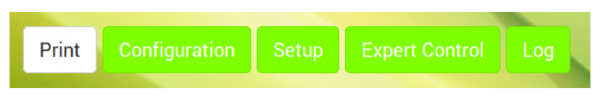
\includegraphics[width=.7\linewidth]{./img/gui_menues_v110.png}
  \caption{Menu selection of the RepRapOnRails operating software.}
\end{figure}

The start-up \emph{Print} screen provides all basic operating functions.
The \emph{Configuration} menu enables the operator to preselect temperature profiles for the extruders and the print bed and build chamber more directly which simplifies preheating and priming according to current needs.
\emph{Setup} offers the operating wizards for guided day-to-day functions.
More advanced features such as program-independent operation of the axes can be found on the \emph{Expert control} screen which also provides direct setting of the extruder temperatures and test extrusion.
The \emph{Log} menu contains the history of machine code input and output as well as the keyboard for direct input of operating instructions.
The following paragraphs provide detailed information of the software's operating screens and explain the specific functions.
Additional information for the preparation of print jobs can be found in Tips and tricks and the manual of the slicing software. 


\subsubsection{[Print] screen}

 After starting the HT500.3 the \emph{Print} screen will appear as the start-up screen. Here you activate the 3D Printer and start the print jobs previously uploaded to the queue via the web interface.

\begin{figure}[H]
  \centering
  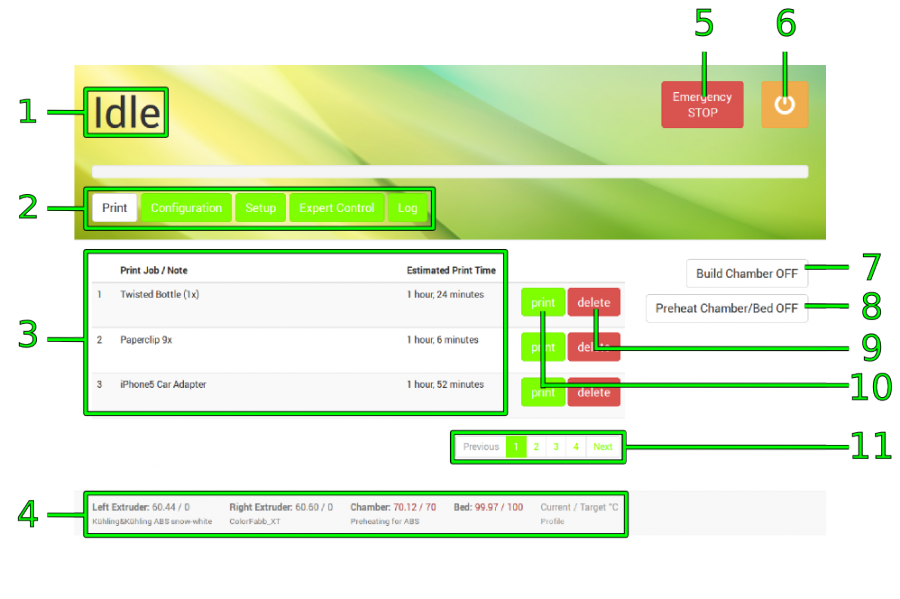
\includegraphics[width=.7\linewidth]{./img/gui_printtabnumber_v110.png}
  \caption{Print screen (descriptions may apply to other screens as well if not 
           explicitly given there)}
\end{figure}

\begin{table}[H]
  \centering
  \begin{tabulary}{\textwidth}{ L L L }
    \toprule
    No.   
      & Description   
        & Content/Function \\
    \midrule
    1   
      & Status message  
        & Idle: apparatus is waiting for next user input \newline
          Printing: apparatus is busy printing  \\
   2  
      & Menu selection  
        & Select the operating menu and mode: 
          Print represents the main production mode \newline
          Configuration allows choosing material based temperature profiles for each extruder and bed/chamber  \newline
          Setup provides wizards for different preset operating procedures
          Expert Control provides access to motors and direct temperature control \newline
          Log represents the communication history of machine\\
   3  
      & Queue   
        & List of uploaded print jobs sorted by time/date (oldest first); estimated 
          time required for printing the respective job. \\
   4  
      & Temperature/profile overview  
        & Displays current and set temperature of each extruder, print bed and build 
          chamber as well as the selected material profiles (see Configuration). Temperatures colored red are set and currently being actuated. \\
   5  
      & [Emergency STOP] button   
        & see also \newline
          $\rightarrow$ Emergency stop \newline
          $\rightarrow$ Safety information in the Manual \\
   6  
      & [Shut-down] button  
        & Tap to shut down the 3D Printer properly. \\
   7  
      & [Build Chamber ON/OFF] button   
        & Tap to activate/deactivate drives and heaters after start-up. \\
    \bottomrule
  \end{tabulary}
\end{table}


\paragraph{Starting print jobs}

Tap the [print] button next to a print job in the queue to start the print job. You will be asked to confirm that all preparations for the print job have been performed. Tap [OK, Start Print] to definitely begin printing or [Cancel] to return to the queue. 

\begin{figure}[H]
  \centering
  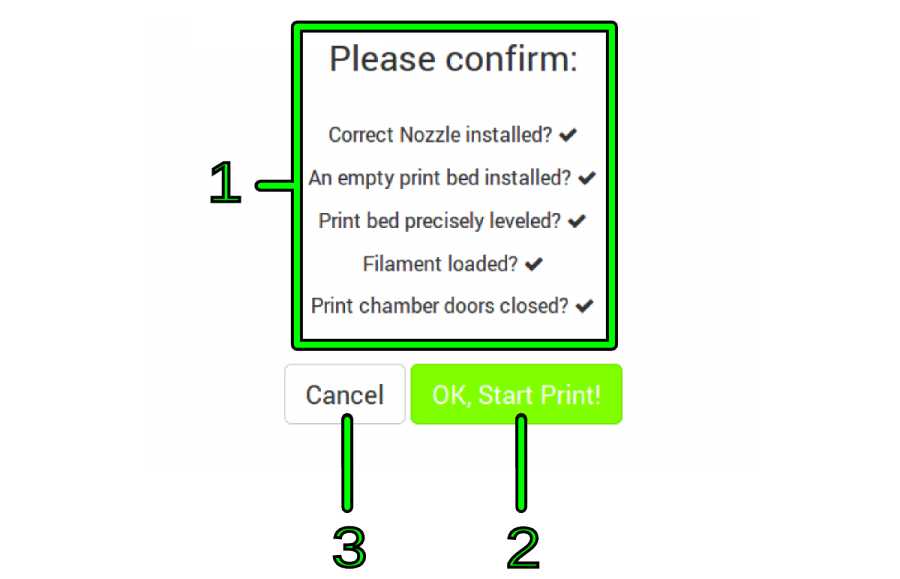
\includegraphics[width=.7\linewidth]{./img/om_confirm_pj.png}
  \caption{“Ready to print?” query}
\end{figure}

\begin{table}[H]
  \centering
  \begin{tabulary}{\textwidth}{ L L L }
    \toprule
    No.   
      & Description   
        & Content/Function \\
    \midrule
    1   
      & Checklist   
        & Please make sure that all displayed requirements have been met before 
          proceeding. \\
    2   
      & [OK, Start Print] button  
        & If all preparations have been made, tap to proceed. \\
    3   
      & [Cancel] button   
        & Tap to abort if any requirements has not been met. \\
    \bottomrule
  \end{tabulary}
\end{table}

After confirmation the HT50.3 starts processing the print job and the status message changes to \emph{Printing}. All other menus are deactivated during a print. The print job name, the current progress, and the estimated remaining time are displayed and the 
[Abort Print] button is active.

\begin{figure}[H]
  \centering
  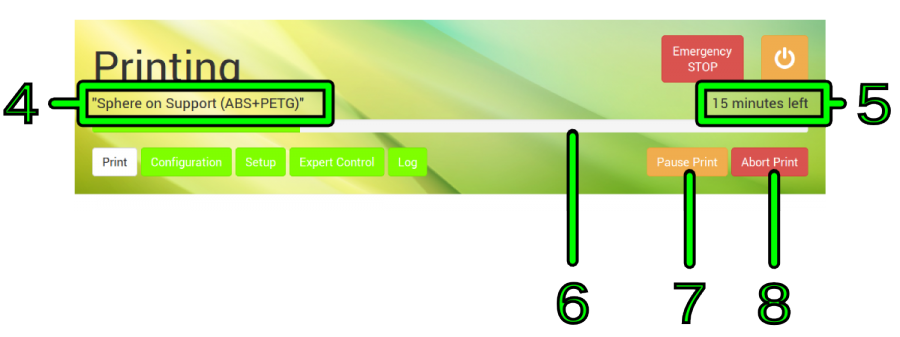
\includegraphics[width=.7\linewidth]{./img/om_currently_printing.png}
  \caption{Print status screen (top half only).}
\end{figure}

\begin{table}[H]
  \centering
  \begin{tabulary}{\textwidth}{ L L L }
    \toprule
    No.   
      & Description   
        & Content/Function \\
    \midrule
    4   
      & Print job name  
        & The name of the slicing file uploaded to the queue. \\
    5   
      & Countdown   
        & Displays the estimated remaining time (calculated from the G-code). \\
    6   
      & Progress bar  
        & Indicates the progress of the print job graphically. \\
    7   
      & [Pause/Resume Print] button   
        & Allows interrupting a print job for interference 
          and subsequent resumption.  \\
    8   
      & [Abort Print] button  
        & Tap to abort a print job. \\
    \bottomrule
  \end{tabulary}
\end{table}


\paragraph{Pause function}

The pause function was built in for the case that a print job needs to be interrupted and later resumed for other reasons than “out-of-filament” (see below).

\begin{figure}[H]
  \centering
  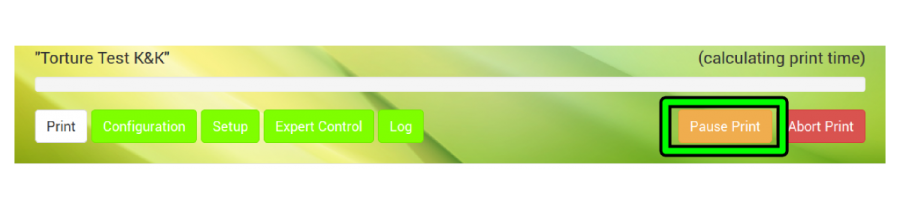
\includegraphics[width=.7\linewidth]{./img/om_pause_print.png}
  \caption{Interrupting the print with the pause function.}
\end{figure}

After tapping the [Pause Print] button, the printer keeps printing until the cache is empty. This may take a few minutes, according to the complexity of the current g-code. Afterwards, the print bed is lowered into its home position, the extruders are turned off and the print head moves to the maintenance position.
Now you have access to the Expert Controls and some of the Setup functions to adjust whatever might be necessary.

\begin{figure}[H]
  \centering
  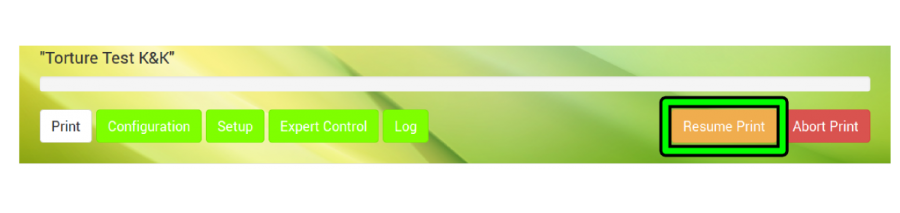
\includegraphics[width=.7\linewidth]{./img/om_resume_print.png}
  \caption{Continuing the print after pause.}
\end{figure}

To continue printing tap [Resume Print] (replaced [Pause Print]). Print bed and extruder head move to their last position and after re-heating the extruders the print continues. 

\paragraph{Finishing a print job}

There are two ways to finish a print job: automatic finish after completion or abortion by the operator.
After regularly completing a print job all axes are moved to their home position and the extruder heating resistors are switched off.
If you need to abort a print job because the outcome does not meet expectations for example or mechanical problems appear during the print, tap the [Abort Print] button. The system will then print the last G-code information from cache and move the print table and the extruder head to their home positions afterwards.
Either way, the 3D Printer returns to idle mode and displays a status message and a request how you wish to continue. Simply tap the respective button on the screen to proceed.
After standstill of all drives you can remove the print bed and take off the model. 

\begin{figure}[H]
  \centering
  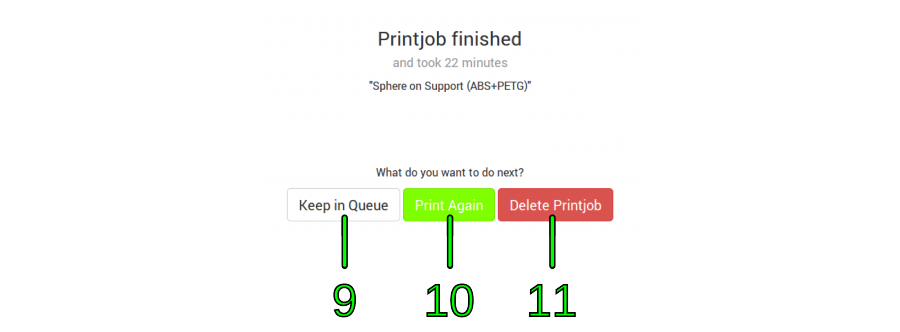
\includegraphics[width=.7\linewidth]{./img/gui_finishedprinting_v110.png}
  \caption{Print job finished.}
\end{figure}

\begin{table}[H]
  \centering
  \begin{tabulary}{\textwidth}{ L L L }
    \toprule
    No.   
      & Description   
        & Content/Function  \\
    \midrule
    9   
      & [Keep in Queue]   
        & Returns to the Print menu. \\
    10  
      & [Print Again]   
        & Immediately restarts the current print job. \\
    11  
      & [Delete Printjob]   
        & Deletes the finished print job from the queue without confirmation and 
          returns to the Print menu. \\
    \bottomrule
  \end{tabulary}
\end{table}


\paragraph{Switching off the 3D Printer}

\begin{notice}
  Switching off the 3D Printer via the power button without turning it into standby may cause damage of the heating elements and neighboring components due to residual heat.
  The cool-down performed during shut-down ensures that the fans are only switched off after the heating elements could shed all residual heat.
\end{notice}

\begin{figure}[H]
  \centering
  \includegraphics[width=.7\linewidth]{./img/om_power_off_button.png}
  \caption{Always use this button for regular shutdown.}
\end{figure}

For switching the HT500.3 into standby tap the shut-down button. The system will then perform the cool-down sequence for safety reasons before deactivating the preheating and the build chamber.

The 3D Printer is in standby mode when:

\begin{itemize}
  \item the screen turns black,
  \item the illuminated ring of the wake button dims,
  \item the build chamber lighting switches off.
\end{itemize}

To wake the machine from standby see $\rightarrow$ emph{Starting the 3D Printer}.. 

For completely shutting down the 3D Printer, perform the procedure described above and set the main switch at the rear cover to \emph{<0>} (OFF) afterwards. The 3D Printer is now powered off.
To reactivate the 3D Printer see $\rightarrow$ emph{Starting the 3D Printer}. 

\begin{info}
  For day-to-day use, the power supply should stay connected to mains power (main switch in position \emph{<I>} (ON). 
\end{info}


\paragraph{Emergency stop}

\begin{notice}
  The emergency stop function does not provide a cool down sequence. \emph{Do not} use the emergency stop button to abort current print jobs, as this may lead to damage of the 3D Printer due to uncontrolled heat accumulation. \emph{Do not} use the main switch as an emergency stop button. You risk loosing or corrupting data. 
\end{notice}

\begin{figure}[H]
  \centering
  \includegraphics[width=.7\linewidth]{./img/gui_v110_emergencystoptriggered.png}
  \caption{Status display after triggering the emergency stop. The 3D Printer 
           returns to IDLE state after a short time. The emergency stop is written into the log-file. }
\end{figure}

When the emergency stop is triggered:

\begin{itemize}    
  \item The machine controller board is reset, all movement of the axes stops, lights, 
        heaters and fans are turned off. The status indicator displays
        \emph{Emergency Stop}!.
  \item After a few seconds the machine controller returns to \emph{Idle} state.
\end{itemize}

The 3D Printer now is in a safe state for troubleshooting.
For repairing \emph{any defects of the electronic equipment or major mechanical damages shut down the 3D Printer completely:}

\begin{itemize}
  \item Shut down the 3D Printer by tapping the \emph{[Shutdown]} button and switching
        off the main switch (\emph{<0>} position) after the shutdown procedure has been finished.
\end{itemize}

\begin{notice}
   Before restarting or reactivating the 3D Printer:
   \begin{itemize}
     \item Make sure that the axes are in no collision position.
     \item Make sure that the reason for the emergency stop has been detected and 
           fixed, before resuming production.
   \end{itemize}
\end{notice}

 After troubleshooting or if the reason for the emergency stop was minor and you want to continue production:

\begin{itemize}
  \item Remove the print bed from the build chamber and replace or clean it before 
        further use.
  \item Restart the 3D Printer (if necessary).
  \item Open the Print screen.
  \item Switch on the build chamber. The 3D Printer will run the homing routine.
  \item You can now resume normal operation.
\end{itemize}


\subsubsection{[Configuration] screen}

 The \emph{Configuration} menu enables you to preselect material-specific temperature profiles for each extruder and, in combination, the print bed/build chamber. The latter is important to make preheating and leveling precise with regard to different material settings. The according profiles can be set up at the web interface setup menu.

\begin{figure}[H]
  \centering
  \includegraphics[width=.7\linewidth]{./img/gui_configmenu_1_v110.png}
  \caption{GUI Configuration screen with temperature profile selection}
\end{figure}

\begin{table}[H]
  \centering
  \begin{tabulary}{\textwidth}{ L L L }
    \toprule
    No.   
      & Description   
        & Content/Function  \\
    \midrule
    1   
      & Left extruder profile selection   
        & The currently selected profile is displayed.
          Tap \emph{[Select]} to open the list of available filament profiles or [Clear] to delete the active profile. \\
    2   
      & Right extruder profile selection
        & same as above \\
    3   
      & Bed/chamber profile selection   
        & The currently selected profile is displayed. 
          Tap [Select] to open the list of available filament profiles or [Clear] to delete the active profile.
          After selection of a profile, deactivate the preheating function in the Print menu (touch button no. 8) and activate it by tapping the button again to apply the settings.  \\
    \bottomrule
  \end{tabulary}
\end{table}

\begin{figure}[H]
  \centering
  \includegraphics[width=.7\linewidth]{./img/gui_configmenu_2_v110.png}
  \caption{The list of chamber/bed temperature profiles of the configuration menu. More 
           profiles can be added via the web-interface.}
\end{figure}

After opening the list, tap [Set] to choose a profile for the selected component. The profile is set and the screen returns to the prior menu.
To activate the selected profile open the Print screen and first deactivate, then re-activate the chamber/bed preheating. 

\begin{figure}[H]
  \centering
  \includegraphics[width=.7\linewidth]{./img/gui_configmenu_3_v110.png}
  \caption{The selected profiles are displayed in the footer of the GUI on every 
           screen.}
\end{figure}

The selected profiles are displayed in the footer of every screen in the order 
\emph{Current} and \emph{Target} (= set) temperature. While aiming for a target temperature, both values are highlighted red. When displayed gray, the temperature value is either not set or currently not triggered.
If no filament profile is activated for an extruder, the default temperature is 
180\degree C. 

\begin{info}
  Observe that the temperature shown in the footer is measured at the hot end heater and may be 5 - 10\degree C lower at the nozzle tip.
  See section \emph{Extrusion temperature} in the knowledgebase for information on finding the suitable extrusion temperature.
\end{info}


\subsubsection{[Setup] screen}

The \emph{Setup} menu displays walkthrough instructions (wizards) for different operations needed during daily operation, initial commissioning, servicing and troubleshooting. If you choose one of the wizards, a step-by-step guide will provide all necessary information for completing the respective task.
This screen also provides system information and the web address needed to connect to the 3D Printer via the network. 

\begin{figure}[H]
  \centering
  \includegraphics[width=.7\linewidth]{./img/gui_setup_wizards.png}
  \caption{Wizard selection on the setup screen. Beginning with ReRapOnRails v1.3.0, 
           the nozzle change wizard has been replaced by the backlash calibration wizard.}
\end{figure}

\begin{table}[H]
  \centering
  \begin{tabulary}{\textwidth}{ L L L }
    \toprule
    No.   
      & Description   
         & Content/Function \\
    \midrule
    1
      & Print Bed Leveling
         & Ensures that print bed and nozzle tip are evenly distanced at every point of the surface.\\
    2
      & Set Extruder Offset
         & Adjust the offset between left and right nozzle for precise alignment in dual-extruder prints.\\
    3
      & Measure Axes Backlash
         & Automatic measurement routine to inspect axes backlash in the drive system. Used for diagnosis 
           in technical support \\
    \bottomrule
  \end{tabulary}
\end{table}

\begin{figure}[H]
  \centering
  \includegraphics[width=.7\linewidth]{./img/gui_setup_info.png}
\end{figure}

\begin{table}[H]
  \centering
  \begin{tabulary}{\textwidth}{ L L L }
    \toprule
    No.   
      & Description   
        & Content/Function  \\
    \midrule
    4   
      & Web Interface URL 
        & Needed to connect to your HT500.3 via the network\\
    5  
      & Version numbers 
        & The valid version numbers of your HT500.3's hardware, the installed 
          RepRapOnRails software and the microcontroller firmware for your information. Please provide these numbers for identification in case of service requests.\\
    \bottomrule
  \end{tabulary}
\end{table}

\subsubsection{[Expert Control] screen}

\begin{notice}
  The Expert Control menu should be used by skilled operators only. Persons unfamiliar with the 3D Printer must not use the functions provided here.
  The positions of the extruder head and the print table are not compared during manual operation. Incautious operation may lead to massive damage of the extruder head and the print bed.
  Be careful not to crash the print table and the extruder head. 
\end{notice}

The [Expert Control] screen provides ability to manually move the X/Y/Z axes of the 3D printer as well as manually setting extruder temperature and priming (eg. for loading/unloading filament)

\begin{figure}[H]
  \centering
  \includegraphics[width=.7\linewidth]{./img/gui_expertmenu_1_v110.png}
  \caption{Expert Control screen}
\end{figure}

\begin{table}[H]
  \centering
  \begin{tabulary}{\textwidth}{ L L L }
    \toprule
    No.   
      & Description   
        & Content/Function \\
    \midrule
    1   
      & Drive control - negative direction  
        & Moves every axis individually once for every tap in negative direction, 
          according to the selected step width. \\
    2   
      & [Printhead Maintenance Position]  
        & Tap to move the extruder head into a preset position in the upper center 
          of the build chamber directly in front of the doors where it is easily accessible for maintenance purposes. \\
    3   
      & Homing buttons  
        & Tap to separately or simultaneously move the axes to their starting 
          positions. \\
    4   
      & Drive control - positive direction  
        & Moves every axis individually once for every tap in positive direction, 
          according to the selected step width. \\
    5   
      & Extruder temperature control  
        & Enables directly setting the temperature and extruding filament for one 
          extruder at a time.  \\
    \bottomrule
  \end{tabulary}
\end{table}


\subsubsection{[Log] screen}

All actions of the machine controller is stored and displayed on the log screen. Print job statuses are stored also.
Direct G-code programming can be effected via the G-code input field. 

\begin{figure}[H]
  \centering
  \includegraphics[width=.7\linewidth]{./img/gui_logmenu_v110.png}
  \caption{The log screen provides additional information about sent and received 
           G-code commands and the possibility of directly influencing the 3D Printer via G-code command input.}
\end{figure}

\begin{table}[H]
  \centering
  \begin{threeparttable}
    \begin{tabulary}{\textwidth}{ L L L }
      \toprule
      No.   
        & Description   
          & Content/Function  \\
      \midrule
      1   
        & History list  
          & communication history sorted top down by date and time \tnote[1] \newline
            SENT: RepRapOnRails host to machine controller\newline
            RECV: machine controller to RepRapOnRails host\\
      2   
        & Browse buttons  
          & Use [Previous], [Next] and [page number] to browse the history.  \\
      3   
        & G-code input field  
          & Enter G-code lines here and [Send] them.  \\
      \bottomrule
    \end{tabulary}
    \begin{tablenotes}\footnotesize
      \item[1] The time is stated in universal time coordinated (UTC) notation so do 
             not wonder if does not match your local time.
    \end{tablenotes}
  \end{threeparttable}
\end{table}
 
\begin{notice}
  The G-code input field is an advanced feature and requires sound knowledge of GCODE programming. Inappropriate use may cause damage to the 3D Printer.
\end{notice}


\subsection{The web interface}

The web interface provides the communication between your PC and the 3D Printer. Uploading print job GCODES to the 3D Printer and creating temperature profiles are the main functions.
You can also check system's information and settings, install firmware updates and download the LOG-file for troubleshooting purposes.

To open the web interface enter the web interface URL into the address line of your internet browser. You can find the web interface URL on the Setup screen of the GUI.

\subsubsection{First Steps}

\begin{figure}[H]
  \centering
  \includegraphics[width=.7\linewidth]{./img/wi_firststeps_printstarted.png}
  \caption{First Steps screen of the web interface.}
\end{figure}

\subsubsection{Queue}

Print jobs are managed via the Queue. Here you can upload GCODES, individaully name, edit, or delete them. 

\begin{figure}[H]
  \centering
  \includegraphics[width=.7\linewidth]{./img/wi_queue_1.png}
  \caption{The Queue contains list of uploaded print jobs in a top-down order with 
           the last upload first.}
\end{figure}

\begin{figure}[H]
  \centering
  \includegraphics[width=.7\linewidth]{./img/wi_queue_2.png}
  \caption{Uploading print jobs to the Queue.}
\end{figure}

To create a print job:

\begin{enumerate}
  \item Click [Add Printjob].
    \begin{enumerate}
      \item Enter the identification (name or number or the like) of the print job in the text field \emph{Name}. This will be shown in the status field during the print job is conducted.
      \item If required, add additional information via the text field \emph{Note}.
    \end{enumerate}
  \item Click [Browse] to select a GCODE from the valid directory.
  \item Click [Add] to upload the selected file to the printer. The print job is 
        added to the list as the first entry.
        Click \emph{[Cancel]} to abort the procedure.
\end{enumerate}

The print job is now available for printing on your HT500.3 and can be selected directly for printing via the touchscreen controller on the 3D Printer.

\begin{figure}[H]
  \centering
  \includegraphics[width=.7\linewidth]{./img/wi_queue_3.png}
  \caption{Editing or deleting print jobs from the web interface queue.}
\end{figure}

\begin{enumerate}
  \item To subsequently renaming print jobs or altering information 
        click on \emph{[edit]} and use the text fields.
  \item To delete a print job from the queue click on \emph{[remove]} and 
        acknowledge the query by clicking \emph{<OK>}.
\end{enumerate}


\subsubsection{Setup}

In the \emph{Setup} menu temperature profiles for materials and print bed/chamber can be managed, system information can be viewed, firmware updates can be conducted and, EEPROM-data can be set. 

\begin{figure}[H]
  \centering
  \includegraphics[width=.7\linewidth]{./img/wi_setup_1.png}
  \caption{Temperature profiles on the Setup screen of the web interface.}
\end{figure}

\begin{figure}[H]
  \centering
  \includegraphics[width=.7\linewidth]{./img/wi_setup_11.png}
  \caption{System information that can also be found on the Setup screen of the GUI. 
           Please always provide these in case you contact the Technical Support. }
\end{figure}

\begin{figure}[H]
  \centering
  \includegraphics[width=.7\linewidth]{./img/wi_setup_12.png}
  \caption{Installing a new machine controller firmware - which may only be done when 
           explicitely requested by Kühling\&Kühling - is done via the Setup menu. Find additional information in the Upgrade section.}
\end{figure}

\begin{figure}[H]
  \centering
  \includegraphics[width=.7\linewidth]{./img/wi_setup_13.png}
  \caption{The EEPROM editor may only be used by experienced users or if explicitely 
           stated in this manual and strictly within the specified parameters. Its main purpose is helping the Technical Support during troubleshooting.}
\end{figure}


\paragraph{Creating temperature profiles}

During a print job all necessary temperature data are provided by the respective G-code. For priming the extruders outside a print job the temperature setting required for extruding a material is provided by the \emph{Filament profiles}.
Similarly, precise print bed leveling needs defined bed and chamber temperatures according to the printed material before a G-code is executed. These settings are provided by the \emph{Chamber/Bed Preheating Profiles}. 

\begin{figure}[H]
  \centering
  \includegraphics[width=.7\linewidth]{./img/wif_setup_addfilamentprofile.png}
  \caption{Filament profile setup via the web interface.}
\end{figure}

To create a filament profile open the web interface of your 3D Printer, choose the Setup menu and:

\begin{enumerate}
  \item Select Filament Profiles and click [Add Profile] to set material properties.
    \begin{enumerate}
      \item Enter the material Name in the according input field.
      \item Enter the Extrusion Temperature in \degree C in the according input field.
    \end{enumerate}
  \item Click [Add] or press <Enter> to save the settings. The new filament profile 
        is added to the list, newest at the bottom.
\end{enumerate}

\begin{itemize}
  \item To change the settings click [edit] and enter the new properties.
  \item To delete a profile click [remove] and confirm the safety query.
\end{itemize}

\begin{figure}[H]
  \centering
  \includegraphics[width=.7\linewidth]{./img/wif_setup_addpreheatingprofile.png}
  \caption{Preheating profile setup via the web interface}
\end{figure}

To create a preheating profile open the web interface of your 3D Printer, choose the Setup menu and: 

\begin{enumerate}
  \item Select Chamber/Bed Preheating Profiles and click [Add Profile] to set 
        material properties.
    \begin{enumerate}
      \item Enter the profile \emph{Name} in the according input field.
      \item Enter the required \emph{Chamber Temperature} in \degree C in the
            according input field.
      \item Enter the necessary \emph{Bed Temperature} in \degree C in the according 
            input field.
    \end{enumerate}
  \item Click [Add] or press <Enter> to save the settings. The new preheating 
        profile is added to the list, newest at the bottom.
\end{enumerate}

\begin{itemize}
  \item To change the settings click [edit] and enter the new properties.
  \item To delete a profile click [remove] and confirm the safety query.
\end{itemize}

\subsubsection{Log}

The Log screen contains the same entries as the Log menu of the GUI. Here you can download the log-file if required for reasons of troubleshooting. A description of the download procedure can be found in the Service Guide. 

\begin{figure}[H]
  \centering
  \includegraphics[width=.7\linewidth]{./img/wi_log_1.png}
  \caption{Download the log-file for support requests via the Log screen.}
\end{figure}
\section{Service guide}

The instructions below are meant to enable you to perform troubleshooting, repair and cleaning tasks adequately and without damaging the machine.

Read the respective guide carefully before you start to work on the HT500.3 3D Printer.


\subsection{Support requests - required information}

 In case you require support and contact us please always provide the following information:

\begin{itemize}
  \item Serial-no.
  \item Hardware revision
\end{itemize}

\begin{figure}[H]
  \centering
  \includegraphics[width=.7\linewidth]{./img/type_plate_ht500-3.png}
  \caption{Finding the hardware revision and serial-no. on the type plate.}
\end{figure}

\begin{itemize}
  \item The .log-file, downloaded via the web interface's Setup tab.
\end{itemize}

\begin{info}
  When downloading the .log-file via the web-interface, please open the \emph{Setup tab first} so that the currently set EEPROM data are written into the log.
  The log file saves all operating and communication commands since the initial commissioning and exports the last 20,000 commands into a data file. Due to this, it may require a few minutes for the system to gather all necessary data before the download menu appears. 
\end{info}

\begin{figure}[H]
  \centering
  \includegraphics[width=.7\linewidth]{./img/wi_v105-v110_logdownload.png}
  \caption{Downloading the log files via the web interface. Please remember opening the Setup tab first.}
\end{figure}

\begin{itemize}
  \item All system information provided on the \emph{Setup} menu. 
\end{itemize}

\begin{figure}[H]
  \centering
  \includegraphics[width=.7\linewidth]{./img/sg_setupmenu_information.png}
  \caption{Please send all system information of the GUI's Setup menu: software version, compatible hardware revision, microcontroller 
           firmware version (compatible and current).}
\end{figure}

Additionally, the following information may be helpful for examining and evaluating your specific request:

\begin{itemize}
  \item Photos of unsuccessful prints often give a clue of what may have gone wrong.
  \item G-codes of above mentioned prints \emph{and} the respective .stl-data allow for reprinting and reproducing your print job and help 
        identifying faults.
  \item Photos and short videos of components, be they damaged or behaving oddly, always provide some clarification.
\end{itemize}



\subsection{Packing and transport safeguarding}

If the HT500.3 is to be shipped (e.g. for a full manufacturer's in-house inspection), it must be thoroughly packed and all moving components must be carefully secured against shifting to avoid transportation damages. 

\begin{info}
   Replacement of parts damaged due to improper transport securing will be carried out at \emph{your costs}. 
\end{info}


\subsubsection{Safeguarding of movable components}

 You will need the following material:

\begin{itemize}
  \item removable strapping tape
        (e.g. tesa® Strapping 64250, Scotch® Strapping Tape 8898 Blue)
  \item packing foam foil
        (any PE-foam for common packing applications)
  \item cardboard
\end{itemize}

The following description assumes that:

\begin{itemize}
  \item all axes are in their respective home position;
  \item filament has been unloaded and the 3D Printer has at least been briefly cleaned;
  \item the 3D Printer has been switched off, disconnected from the power supply and cooled down;
  \item all cables have been removed from the rear side.
\end{itemize}



The first and most important component to be secured is the extruder head. It is \emph{mandatory} to fix it exactly as shown here. Otherwise sensors and other components may be damaged beyond repair and must be replaced.

\begin{itemize}
  \item Move the H-gantry to the front and the extruder head to the right-hand side.
  \item Place a foam coil between the extruder head and the right X-axis shaft carriage and push the extruder head against the coil.
  \item Fasten the extruder head together with the carriage by entwining them with strapping tape.
  \item Make sure to tension the tape so that any extruder head movement is prevented.
\end{itemize}

 

\begin{figure}[H]
  \centering
  \includegraphics[width=.7\linewidth]{./img/packstep0.png}
  \caption{Move the extruder head to the front and to the right.}
\end{figure}

\begin{figure}[H]
  \centering
  \includegraphics[width=.7\linewidth]{./img/secure_extruderhead.png}
  \caption{Cushion the extruder head with the foam coil against the right carriage and tightly fasten it with tape.}
\end{figure}

\begin{itemize}
  \item Fasten the energy chain to the printer top cover. 
\end{itemize}

\begin{figure}[H]
  \centering
  \includegraphics[width=.7\linewidth]{./img/secure_echain.png}
  \caption{Entwine the e-chain with tape and fasten it to the printer's top cover.} 
\end{figure}

\begin{itemize}
  \item Fix the H-gantry with strapping tape against forward movement by fastening it to one of the Z-Axes. 
\end{itemize}

\begin{figure}[H]
  \centering
  \includegraphics[width=.7\linewidth]{./img/secure_hbridge_rear.png}
  \caption{Entwine the hind shaft of the H-gantry with tape and fasten it to on of the Z-axes.}
\end{figure}

\begin{itemize}
  \item Fix the H-gantry with strapping tape against backward movement by fastening it to the printer top cover.
  \item Make sure to tension the tape to prevent forward/backward movement of the H-bridge. 
\end{itemize}

\begin{figure}[H]
  \centering
  \includegraphics[width=.7\linewidth]{./img/secure_hbridge_front.png}
  \caption{Entwine the frontal shaft of the H-bridge with tape and fasten it to the printer's top cover.}
\end{figure}

\begin{itemize}
  \item Cut and prepare a cardboard support as depicted.
  \item Place the support underneath the print table and fix it with strapping tape.
\end{itemize}

\begin{figure}[H]
  \centering
  \includegraphics[width=.7\linewidth]{./img/img_1708.jpg}
  \caption{The cardboard support installed at delivery is the best option to secure the print table.}
\end{figure}

\begin{figure}[H]
  \centering
  \includegraphics[width=.7\linewidth]{./img/secure_printtable.png}
  \caption{Place the cardboard support underneath the print table and fix it with tape.}
\end{figure}

\begin{itemize}
  \item Close the build chamber doors and fix them with strapping tape as shown.
  \item Wrap the touchscreen with foam foil and fixate it with strapping tape.
\end{itemize}


\begin{figure}[H]
  \centering
  \includegraphics[width=.7\linewidth]{./img/secure_doors_gui.png}
  \caption{Tape the doors and wrap the touchscreen with foam foil.}
\end{figure}


\subsubsection{Packing for transport}

After safeguarding, the 3D Printer is ready for packing. You will need the following material:

\begin{itemize}
  \item 4x lashing strap or tension belt
  \item closed surface transport pallet
  \item packing foam foil
  \item 4x anti-slip mats 50 x 50 mm (only 3D Printers without rubber feet)
  \item OSB transport top cover (or similar) 700 x 700 x 25 mm
  \item delivery transport box side cover frame
  \item delivery transport box lid
\end{itemize}

The description refers to using the original transport box the 3D Printer was delivered in. If you disposed of the box, make sure to provide adequate replacement.

\begin{itemize}
  \item Lift the 3D Printer onto the center of the pallet.
  \item Place a suitable piece of transport foam foil on top of the 3D Printer.
\end{itemize}

\begin{notice}
  To avoid damage by slipping, place anti-slip mats under the feet if your 3D Printer is not already equipped with rubber feet.
  \begin{figure}[H]
    \centering
    \includegraphics[width=.7\linewidth]{./img/packstep3.png}
  \end{figure}
\end{notice}

\begin{figure}[H]
  \centering
  \includegraphics[width=.7\linewidth]{./img/packstep1.png}
  \caption{Place the 3D Printer in the middle of the pallet and cover it with foam foil.}
\end{figure}

\begin{itemize}
  \item Place the cover plate on top of the 3D Printer. 
\end{itemize}

\begin{figure}[H]
  \centering
  \includegraphics[width=.7\linewidth]{./img/packstep4.png}
  \caption{The cover plate protects the printer when strapping it down.}
\end{figure}

\begin{itemize}
  \item Fasten the 3D Printer with two lashing straps to the pallet.
\end{itemize}

\begin{figure}[H]
  \centering
  \includegraphics[width=.7\linewidth]{./img/packstep5.png}
  \caption{The 3D Printer must be tightly secured on the transport pallet.}
\end{figure}

\begin{itemize}
  \item Lift the side cover frame onto the pallet.
  \item Make sure that the grove of the pallet fits smoothly.
\end{itemize}

\begin{figure}[H]
  \centering
  \includegraphics[width=.7\linewidth]{./img/packstep6.png}
  \caption{The side cover frame must be accurately positioned to protect the 3D Printer from damage.}
\end{figure}

\begin{itemize}
  \item Close the box with the lid.
  \item Make sure that the lid smoothly fits into the side cover frame. 
\end{itemize}

\begin{figure}[H]
  \centering
  \includegraphics[width=.7\linewidth]{./img/packstep7.png}
  \caption{Ensure the lid fits so that tensioning the lashing straps will work.}
\end{figure}

\begin{itemize}
  \item Secure the transport box with two lashing straps on the pallet.
  \item Attach all necessary labeling on the outside:
    \begin{itemize}
      \item dispatch note
      \item UP sticker (present on the original transport box)
      \item FRAGILE sticker (present on the original transport box)
      \item PROTECT FROM WEATHER EFFECTS (if required, present on the original transport box)
    \end{itemize}
\end{itemize}

\begin{figure}[H]
  \centering
  \includegraphics[width=.7\linewidth]{./img/packstep8.png}
  \caption{The HT500.3 3D Printer is packed and ready for transportation 
           after lashing straps have been tightened and all labeling has been attached.}
\end{figure}



\subsection{Hardware components and manual tasks}


\subsubsection{Maintenance Intervals}

\paragraph{Daily (end of shift)}

\begin{table}[H]
  \centering
  \begin{tabulary}{\textwidth}{ L L L }
    \toprule
    Where          &	    What                      &	 	Tools / To Do \\
    \midrule
    Build chamber  &	 	remove filament residues  &	 	brush, hand broom, vacuum cleaner \\
    \bottomrule
  \end{tabulary}
\end{table}    

\paragraph{Monthly (150 operating hours)}  

\begin{table}[H]
  \centering
  \begin{tabulary}{\textwidth}{ L L L }
    \toprule
    Where               &	  What                                                     &	 Tools / To Do \\
    \midrule
    Timing belt         &	  check the tension; re-tension if required                &	 $\rightarrow$ section \ref{sec:belttension} \\
    Shafts              &	  check for dryness; lubricate if required                 &	 $\rightarrow$ section \ref{sec:lubrication} \\
    Cooling circuit     &	  check hoses for excessive bubbles; refill if required    &   $\rightarrow$ section \ref{sec:coolant} \\
                        &	  check hose connectors at the LEDs and 
                              the stepper drives for correct positioning; 
                              refasten if required 	                                   &                  \\
    Dust wiping sponge  &	  check for cleanliness; 
                              clean or replace if required                             &  rinse with fresh water
                                                                                          and dry thoroughly \\
    \bottomrule
  \end{tabulary}
\end{table}


\paragraph{Yearly (2.500 operating hours)}

\begin{table}[H]
  \centering
  \begin{tabulary}{\textwidth}{ L L L }
    \toprule
    Where             &     	  What                                                   &	 Tools / To Do \\
    \midrule
    Z-axis 
    spindle drive 	  &  check for fast seat:\newline
                         with the 3D Printer switched on, grab the print table near
                         the elevator and try to lift it\newline
                         $\rightarrow$ play of the table on  the spindle requires 
                         replacement of the spindle nut\newline                                  
                         $\rightarrow$ if you can lift the entire assembly including 
                         the spindle, the adjusting rings must be refastened 	         &   $\rightarrow$ section \ref{sec_spindlecollar}  \\
    \bottomrule
  \end{tabulary}
\end{table}

\subsubsection{Cleaning recommendation}

\begin{danger}
   OF INJURY\\
   Some plastics need very aggressive solvents that may cause intoxication, caustic burns, skin, eye and/or mucosal irritations, allergic reactions and other medical consequences. Solvents may emit flammable or toxic vapors or be corrosive.
   To avoid injuries and accidents due to use of solvents:

   \begin{itemize}
      \item Always observe the safety information provided in the manufacturer's safety data sheet concerning
            possible dangers, handling and adequate storage.
      \item Always wear adequate protective equipment.
      \item Do not use solvents in a surrounding not suited to the task. If required, 
            adequate aeration or exhaust ventilation has to be provided.
      \item Always use adequate containers for handling and storing solvents.
      \item It is the owner's responsibility to provide any necessary equipment and protective gear 
            for every person operating the HT500.3 3D Printer.
  \end{itemize}
\end{danger}

\begin{danger}
  OF BURNING\\
  The build chamber interior may reach temperatures of up to 70\degree C (158\degree F), the print bed may reach temperatures up to 130\degree C (266\degree F) and 
  the hot ends may reach temperatures up to 300\degree C (572\degree F). Touching components can cause burning injuries ranging from burn blisters to medium aching burns. Before cleaning any component inside the build chamber:
  
  \begin{itemize}
    \item Move the print head to the maintenance position 
          (GUI $\rightarrow$ \lbrack Expert Control\rbrack  $\rightarrow$ \lbrack Print Head Maintenance Position \rbrack  ).
    \item Switch preheating of the 3D Printer off 
          (GUI $\rightarrow$ \lbrack Print\rbrack  $\rightarrow$ \lbrack Preheat Chamber/Bed OFF\rbrack  ).
    \item Let the printer cool down to at least 52\degree C.
  \end{itemize}
\end{danger}

\begin{notice}  
  Acetone is the most effective solvent for ABS and thus recommended for most cleaning purposes at the HT500.3 3D Printer.
  To remove residues of other plastics than ABS, refer to the respective manufacturer's data sheet for suitable solvents.

  Regard the following when using solvents for cleaning purposes:

  \begin{itemize}
    \item Do not use solvents inside the build chamber. They may evaporate and produce fumes that can dissolve plastic 
          components (e.g. the energy chain links) and printed objects. Always remove components from the build chamber before treating them with a solvent and dry thoroughly before re-insertion.
    \item Do not use liquids inside the build chamber. These may enter the electronic chamber and cause short circuits or
          otherwise damage electronic components.
  \end{itemize}
\end{notice}


\paragraph{Housing}

Although during normal operation it is not necessary to clean the 3D Printer daily, regularly dusting reduces the probability of dust entering the feed system and causing clogging. Also, the visual appearance of the 3D Printer is improved and damaged components are more easily detected.
All components of the HT500.3s' housing can be cleaned with mild household detergents (e.g. dish soap, glass cleaner) and lint-free towels.
\emph{Do not} use abrasive detergents or scouring pads as these will scratch and blind the acrylic glass covers and the touchscreen surface.
Material residues should be removed routinely from the build chamber. Use a soft brush or a low-running vacuum cleaner to remove loose material shreds.

\paragraph{Touchscreen}

If required, use a microfiber or spectacle cloth moistened with glass cleaner to wipe the touchscreen.

\paragraph{Print bed}

PEI is highly resistant to a lot of solvents. It is particular compatible with acetone and isopropyl alcohol. If you experience insufficient adhesion of objects to the surface during prints, it is advisable to thoroughly clean the print bed with an acetone-soaked lint-free cloth.

Grease residues on the surface of the print bed (i.e. fingerprints) can lead to poor adhesion. To degrease, apply isopropylalcohol to a lint-free cloth and thoroughly wipe the surface. During further use, regular removal of grease residues with isopropyl alcohol will prevent poor adhesion.

Use acetone as solvent to remove ABS residues from the print bed. Apply the acetone to a cloth and wipe the print bed rather than dousing it directly.

Other material's residues are best removed with a lint-free towel soaked in a suitable, non-corrosive, non-toxic solvent. Observe the manufacturer's safety data sheet when handling plastic solvents. Make sure to thoroughly wash off any residues. Remaining smear may lead to increased adhesion, which can render it impossible to release printed objects without damage.

\paragraph{Hot ends}

Cleaning the hot end nozzle tip is required quite often compared to other components of the 3D Printer. Dust ingression through the filament supply system, coking of material, and storage in a dusty place may lead to clogging of the tip's bore.
An imprecisely (too closely) leveled print bed, too low extrusion temperatures or too high an extrusion speed can lead to the nozzle tip choking itself.
In any of these cases, a decreasing print quality and slipping of the drive gear will be the first visible effects. Removing and cleaning the nozzle tip is then necessary; the description below should remedy the problem, as long as no hardware defect is present.

Cleaning the extruder nozzle is only required if it is clogged with coked material or foreign particles. It is recommended after dissembling the hot end at material change (installing a \emph{different} material). 

\begin{info}
  In areas with high dust formation, \underline{especially} from textile fibers and similarly flexible particles, the risk of the nozzles to become clogged is highly increased.
\end{info}

\paragraph{Filament drive gear}

Slipping of the drive gear is almost always the first and visible consequence of a clogged nozzle.
Other conditions (e.g. too high idler tension) may also cause the drive gear to grind into the filament and fill with abrasion. Material transport will stop and the print job will not be finished.
Regard that the printer will nevertheless continue to print if not aborted by the operator.
Clean according to the description below

\begin{figure}[H]
  \centering
  \includegraphics[width=.7\linewidth]{./img/mtc_cleangeardrive.png}
  \caption{Filament abrasion at the drive gear due to slipping.}
\end{figure}

\subsubsection{Changing the filament} \label{sec:filamentchange}

When the filament limit switch at the filament supply registers the end of the filament strand on the spool, the 3D Printer stops automatically and signals lack of material at the touchscreen.
If you want to remove the filament for other reasons (e.g. to use a differently colored material), the following description applies also.


\paragraph{Required tools}

\begin{itemize}
  \item diagonal cutters
\end{itemize}


\paragraph{Unloading Filament}


\begin{enumerate}
  \item Go to the \emph{[Expert Control]} menu and heat up your extruder to melting temperature.
  \item Pull the filament feeding tube out of the extruder idler lever about 3cm.
  \item Cut the filament with wire cutters about 1cm above the extruder idler lever.
  \item Cut the filament with wire cutters between filament feed insert and
        filament spool at the back of the machine.
  \item From inside of the build chamber, pull the separated strand of filament out of 
        the feeding tube.
  \item Pivot the filament idler wheel away from the filament drive gear with two fingers,
        and pull the remaining filament section upwards out of the nozzle.
  \item In the \emph{[Expert Control]} panel, switch your extruder heater OFF again.
\end{enumerate}


\paragraph{Loading Filament}

If you want to continue printing with another type of plastic (e.g. PETG instead of ABS) than has previously been used in the currently installed nozzle, you need to change the extruder nozzle before loading the filament.

\begin{info}
  Using the same extruder nozzle for materials with different properties may lead to clogging of the nozzle tip due to coking or sooting.
  Kühling\&Kühling recommend either thorough cleaning of the extruder nozzle with a suitable solvent and pipe cleaners or using a single nozzle for every type of material.
\end{info}

\begin{enumerate}
  \item Unload the current filament as described in the previous paragraph.
  \item Subsequent to unloading you have to change the extruder nozzle as 
        described in the Service guide.
  \item Install a new spool of filament by sliding it onto the spool holder at the back of
        the machine. Adjust the spool carrier to fit.
  \item Pull the filament feed tube out of the extruder idler lever.
  \item Cut off the beginning of the filament with wire cutters to get a
        straight end.
  \item Lead the plastic rod into the filament feed until it protrudes the feeding tube
        about 10cm at the other side (at the extruder).
  \item Relax the filament idler wheel tension with two fingers.
        Then feed the filament from top through the idler lever,
        down into the nozzle.
  \item Go to the \emph{[Expert Control]} menu and heat up your extruder to melting temperature.
  \item Use the \emph{extrude} controls to manually prime the nozzle until a consistent, smooth strand of extruded material
        flows out of the nozzle tip.
  \item In the \emph{[Expert Control]} panel, switch your extruder heater OFF again.
\end{enumerate}

\begin{info}
  Make sure to choose the appropriate filament profile from the material database.
\end{info}


\subsubsection{Adjusting the spool carriers}

\paragraph{Required tools}
 
\begin{itemize}
  \item Allen wrench \#2.5
\end{itemize}

\paragraph{Procedure}

If you want to use a different filament spool diameter (less or more material), you have to adjust the spool carrier position.

\begin{info}
  With an appropriate Allen key you can carry out the following steps without removing the filament spool.
\end{info}
\begin{itemize}
  \item Use the Allen key to loosen the fixing screws of the carrier.

  \begin{figure}[H]
    \centering
    \includegraphics[width=.7\linewidth]{./img/mtc_filamentmovespools.png}
    \caption{Loosening the fixing screws of spool carriers.}
  \end{figure}

  \item Slide the carrier to or away from the filament inlet to a position that 
        leaves approximately 1 cm between the spool's outer rim and the limit switch. Make sure that the filament enters the inlet at an angle 
        of 85-90\degree.
  \item Refasten the fixing screws.

  \begin{figure}[H]
    \centering
    \includegraphics[width=.7\linewidth]{./img/mtc_filamentinletmeasures.png}
    \caption{Admissible distance and inlet angle.}
  \end{figure}

\end{itemize}


\subsubsection{Remedying clogging}

\paragraph{Required tools}

\begin{itemize}
  \item dental pick hook or needle
  \item material specific solvent
  \item pipe cleaner
\end{itemize}

\paragraph{Procedure}

\begin{itemize}  
  \item Unload the filament ($\rightarrow$ section \ref{sec:filamentchange}).
  \item Screw off the nozzle.
  \item Roughly remove material residues mechanically (e.g. using a brass wire brush - wear protective goggles!).
  \item Drop the nozzle tip into a suitable solvent and wait for the residues to be loosened or completely dissolved.
  \item Remove remaining material mechanically.
  \item Dry the nozzle thoroughly before re-installation.
\end{itemize}

To remove particles and abrasion from the feed system:

\begin{itemize} 
  \item Remove the filament strand from the supply system.
  \item Take out the dust wiping sponge from the filament inlet, rinse it with water, and dry it thoroughly.
  \item  Scrape the teeth of the drive gears with a pointed tool (e.g. dental pick).
  \item  Reinstall the supply hoses and the dust wiping sponge.
\end{itemize}

\paragraph{Completion}

After having re-installed or exchanged all components, 
reload the filament, prime the extruders and run the \lbrack Print bed leveling\rbrack  wizard. 


\subsubsection{Shaft lubrication} \label{sec:lubrication}

All linear bearings of the HT500.3 are equipped with linear ball bearings. The shafts may accumulate dirt or condensation. Slightly Lubricating/Cleaning the shafts may then be necessary.

\paragraph{Required tools}

\begin{itemize}
  \item \emph{HIWIN Type G05} bearing grease
  \item paper towel or lint-free cloth
\end{itemize}

\begin{notice}
  Do not use any other lubricant. The linear bearings may get irreparably damaged when greased falsely. 
\end{notice}

\paragraph{Applying lubricant}

If you notice strong vibrations of the print table during homing and leveling or if your printed objects show increasingly rough vertical irregularities:

\begin{itemize}
  \item Wipe shafts clean with a paper towel.
  \item Coat the shafts with a thin layer of the lubricant.
\end{itemize}

\subsubsection{Opening the electronic chamber}

To access the cooling system or the control elements, you have to remove the left or the right side cover panel. The description below applies to either side. 

\begin{danger}
  ELECTRIC SHOCK HAZARD\\
  Electric shock can cause severe injuries. Never open the electronic chamber when the 3D Printer is powered on.
  Always shut down and power off the 3D Printer and disconnect the power supply before removing covers and working on electronic components. Allow the power supply to discharge for at least one minute. 
\end{danger}

\begin{notice}
  Electrostatic discharge can damage electronic components. Ground yourself before touching electronics. 
\end{notice}

\paragraph{Required tools}
\begin{itemize}
  \item Allen wrench \#2.5 
\end{itemize}

\paragraph{Additional information}

Software manual

\paragraph{Removing}

Shut down the printer via the touchscreen panel, switch off the main power switch and unplug the supply cable. Open the electronic chamber of the 3D Printer in the following sequence:

\begin{itemize}
  \item Slightly tilt the apparatus to the opposing side and place a square length of wood underneath the bottom.
\end{itemize}

\begin{danger}
  OF CRUSHING\\
  Capsizing of the 3D Printer can cause crushing injuries and damage the housing beyond repair. Make sure the apparatus does not topple. 
\end{danger}

\begin{itemize}
  \item Loosen (\emph{do not remove}) the hexagon socket screws of the feet and the upper hind cover angle.
  \item Turn the hammerhead nuts by 90\degree.
  \item Remove the feet and the angle.
  \item Loosen (\emph{do not remove}) the hexagon socket screws of the cover panel.
  \item Turn the hammerhead nuts by 90\degree.
  \item Remove the cover panel.
  \item Loosen all screws around the white acrylic side panel and take the panel off. 
        You now have access to the electronics driving the HT500.3.
\end{itemize}

Reinstall in reverse order, remove the wood and restart.

\begin{figure}[H]
  \centering
  \includegraphics[width=.7\linewidth]{./img/sg_openechamber_1.png}
  \caption{Lift the 3D Printer at one side; the feet and the hind cover angle must be removed.}
\end{figure}

\begin{info}
  You want to keep the t-slot nuts on the thread – otherwise they might fall into the slot, which can require further disassembling of the printer to get it back out.
\end{info}

\begin{figure}[H]
  \centering
  \includegraphics[width=.7\linewidth]{./img/open_electronics_enclosure_-_step4_-_02.png}
\end{figure}

\begin{figure}[H]
  \centering
  \includegraphics[width=.7\linewidth]{./img/open_electronics_enclosure_-_step4_-_03.png}
\end{figure}

\begin{figure}[H]
  \centering
  \includegraphics[width=.7\linewidth]{./img/open_electronics_enclosure_-_step4_-_04.png}
\end{figure}

\begin{figure}[H]
  \centering
  \includegraphics[width=.7\linewidth]{./img/open_electronics_enclosure_-_step5_-_02.png}
\end{figure}

\begin{figure}[H]
  \centering
  \includegraphics[width=.7\linewidth]{./img/open_electronics_enclosure_-_step5_-_03.png}
\end{figure}

\begin{figure}[H]
  \centering
  \includegraphics[width=.7\linewidth]{./img/open_electronics_enclosure_-_step5_-_01.png}
\end{figure}

\subsubsection{Changing the nozzle tip}

Printing with another nozzle diameter, cleaning or change of material all requires unscrewing and remounting the nozzle tip. Although not a complicated procedure, make sure to read the following description thoroughly to avoid damaging the hot-end. 

\begin{danger}
  BURNING HAZARD\\
  Before unscrewing a nozzle, the filament must be removed from the hot-end which may require heating to extrusion temperature. Depending on the installed material temperatures up to 300\degree C may be necessary that can cause severe burns.

  \begin{itemize}
    \item Be careful not to touch hot components.
  \end{itemize}
\end{danger}

\paragraph{Required tools}

\begin{itemize}
  \item open-jaw wrench size 4
\end{itemize}

\paragraph{Removing the nozzle}

After the extruder has cooled down:

\begin{itemize}
  \item Open the <Expert Control> menu, tap the \lbrack Printhead Maintenance Position\rbrack  button 
        and wait until the print head has moved to the middle front position.
  \item Check nozzle adapter thumb screw for tightness.
\end{itemize}


\begin{notice}
  If solidified material hinders loosening the nozzle effortlessly, heat up the extruder to the specific extrusion temperature and loosen the tip 2 or 3 turns. Do not unscrew the heated nozzle totally. Dropping the hot nozzle will damage the acrylic bottom. Afterwards, turn the extruder off and wait until it has cooled down before completely removing the nozzle. 
\end{notice}

\begin{itemize}
  \item Loosen and remove the nozzle with a size 4 wrench at the width flat of the nozzle. Carefully slide the nozzle out of
        the heating element.
\end{itemize} 

\paragraph{Installing a new nozzle}

\begin{itemize}
  \item Slide a new nozzle into the heating element.
  \item Screw the nozzle into the nozzle adapter. 
  \item Carefully fasten the nozzle with a size 4 wrench.
  \item Run the Print Bed Leveling wizard. 
\end{itemize} 


\subsubsection{Refilling the cooling circuit} \label{sec:coolant}

Thermal cycles and diffusion of the coolant makes refilling the cooling circuit necessary approximately every four weeks. To refill the coolant circuit, follow the instructions given below. 

\paragraph{Required tools}

\begin{itemize}
  \item Coolant Innovatek Protect IP ready-to-use \footnote{Order directly via sales@kuehlingkuehling.de, 
        the manufacturer's webshop (http://innovatek.de, manufacturer part number: 500473) or related distributors.} 
        (max. 250 ml)
  \item Allen wrench \#2.5
\end{itemize}

\paragraph{Checking the cooling circuit}

\begin{info}
  Lack of coolant may lead to damage of the affected components, especially the LEDs. Too much air in the cooling circuit leads to clogging of the copper connectors due to oxidation.
  Check the cooling circuit regularly for excess amounts of gas bubbles.
\end{info}

The amount of gas bubbles in the cooling circuit is the indicator for refilling. A small amount of bubbles always circles the hoses and can be considered normal. To asses whether the cooling circuit must be refilled, check the following:

\begin{itemize}
  \item The bubbles are small and running freely $\rightarrow$ there is no need for refilling the cooling circuit.
  \item Bubbles reach the size of the hose's diameter, are sticking in places and do not disappear 
        a few minutes after switching the build chamber on $\rightarrow$ refill as described below.
\end{itemize}

\paragraph{Refilling the pump}

\begin{enumerate}
  \item Locate the water pump at the rear of the machine.
  \item Remove the pump's lid by turning it counterclockwise and pulling it off.
  \item Refill with coolant up to the level indication.
  \item Let the pump run for some minutes. Monitor the coolant hoses and check that air bubbles run freely.
        If necessary, carefully flick the hoses to free trapped air. When all air bubbles have left the cooling system, check the filling level of the pump again and refill to the upper limit.
  \item Press the lid into the housing and turn it clockwise. Make sure the lid is positioned fast 
        in its seat and locked.
\end{enumerate}

\begin{figure}[H]
  \centering
  \includegraphics[width=.7\linewidth]{./img/waterpump_rear.png}
  \caption{Cooling water pump accessible at the rear of the machine.}    
\end{figure}

\begin{figure}[H]
  \centering
  \includegraphics[width=.7\linewidth]{./img/mtc_coolingwaterpumpopenlid.png}
  \caption{Opening/closing the pump's lid.}
\end{figure}

\begin{figure}[H]
  \centering
  \includegraphics[width=.7\linewidth]{./img/mtc_coolingwaterpumprefill.png}
  \caption{Level indication of the cooling water pump.}
\end{figure}


\subsubsection{Extruder idler lever}

\paragraph{Required tools}

\begin{itemize}
  \item Allen wrench \#3 
\end{itemize}	

\paragraph{Adjusting the preload}

At delivery, the idler lever preload is preset to work with the standard material \emph{Kühling\&Kühling ABS}. To print other plastics it may be necessary to adjust or readjust the tension of the idler lever spring. 

\begin{info}
  The preset value can be read as the distance in mm between the underside of the set screw and the underside of the extruder head carrier. It is set to 5.4 mm at delivery for ABS.
  \begin{figure}[H]
    \centering
    \includegraphics[width=.7\linewidth]{./img/mtc_idlerleverpreset.png}
  \end{figure}
\end{info}

Too high tension of the idler lever spring may result in the gear drive to slip and grind into the filament. Too low tension of the idler lever spring may result in slipping of the gear drive. In both cases the print will abort due to insufficient material transport.
Adjust the idler lever spring pressure by turning the tensioning screw with a metric \#3 Allen key, just enough that the filament is transported reliably without slipping or chipping. Turn the screw clockwise to increase the preload and counterclockwise to decrease it.
To test material transport efficiency run the Prime Extruders wizard and readjust if necessary. 

\begin{figure}[H]
  \centering
  \includegraphics[width=.7\linewidth]{./img/mtc_springload.png}
  \caption{Adjusting the idler lever preload.}
\end{figure}

\begin{info}
  Be gentle, too much pressure is counterproductive and will result in chipping filament.
\end{info}

\subsubsection{Timing Belt Tension} \label{sec:belttension}

The Tension of the X-axis and both Y-axis timing belts can be checked by measuring the resonance frequency when plucked like a guitar string.

\begin{itemize}
  \item Activate the build chamber preheating and wait until the 3D Printer 
        has reached its operating temperature (eg. 70\degree C for printing ABS).
  \item Then pluck the longest free hanging section of a belt and measure the oscillation with a frequency meter.
        Make sure to be as close to the belt as possible with the microphone of your device.
  \item Adjust by rotating the knurled thumb-wheels on each belt tensioner 
        until a frequency of about 60 Hz ($\pm$ 5 Hz) is met.
  \item Repeat this procedure for all belts.
\end{itemize}

\begin{figure}[H]
  \centering
  \includegraphics[width=.7\linewidth]{./img/mtc_belttension.png}
  \caption{Knurled thumb-wheels on belt tension}
\end{figure}

\begin{info}
  A guitar tuning device will be sufficient - also available as smart phone app.
\end{info}


\subsubsection{Repositioning and refastening the Z-axis clamp collar} \label{sec_spindlecollar}

During transport or set up verberation may lead to loosening of set screws. If this happens at the upper clamp collar of the Z-spindle, the initial Z-positioning of a print job becomes inaccurate \emph{although the leveling seems OK} because the spindle's mechanical backlash will then avert exact positioning only during minimal lifting moves. You will find that the first layer will not stick to the print bed as if it was leveled too high.
In this case the clamp collar must be repositioned and the set screw must be refastened. 

\paragraph{Required tools}

\begin{itemize}
  \item Allen key \#2.5
\end{itemize}

\paragraph{Testing and repositioning the clamp collars}

\begin{danger}
  OF BURNING\\
  Depending on the printed material components of the 3D Printer may hold 
  temperatures up to 500\degree C (932\degree F) immediately after a print job.
  To avoid burning injuries:

  \begin{itemize}
    \item Switch off the preheating and wait until the 3D Printer 
          has cooled down to approximately 50\degree C (122\degree F).
    \item Check the current temperature at the display.
  \end{itemize}
\end{danger}

\begin{info}
  Lifting the print table at the front end may damage the Z-elevator assembly and the spindle. Also, leverage effects might effect a false impression of alleged play.
  Grab the print table at the Z-elevator near the bearings when trying to lift it.
  Make sure that you do not damage the Z-limit switch. 

  \begin{figure}[H]
    \centering
    \includegraphics[width=.7\linewidth]{./img/mtc_liftelevatorincorrect.png}
  \end{figure}
\end{info}

To test if the clamp collar has come loose, carefully try to lift the print table and observe the Z-drive pulley.
If the pulleys moves up and down, the clamp collar must be repositioned and the set screws refastened. 

\begin{figure}[H]
  \centering
  \includegraphics[width=.7\linewidth]{./img/mtc_liftelevatorwatchpulley.png}
  \caption{Try to lift the Z-elevator and watch the pulley. If the pulley moves up and down, 
           the clamp collar must be repositioned.}
\end{figure}

To reposition the clamp collar:

\begin{itemize}
  \item Carefully turn the spindle of the Z-drive manually so that the recess of the clamp collar points left.
    
    \begin{figure}[H]
      \centering
      \includegraphics[width=.7\linewidth]{./img/mtc_z-axis_alignclampcollar.png}
      \caption{Align the recess of the clamp collar parallel to the 3D Printer's front.}
    \end{figure}

  \item Loosen the set screw through the access bore in the carriage.

    \begin{figure}[H]
      \centering
      \includegraphics[width=.7\linewidth]{./img/mtc_z-axis_loosensetscrew.png}
      \caption{Use the \#2 Allen key to loosen the set}
    \end{figure}

  \item Hold down the Z-pulley and push the clamp collar up to the limit.
  \item Hold the clamp collar in place and fasten the set screw tightly.

    \begin{figure}[H]
      \centering
      \includegraphics[width=.7\linewidth]{./img/mtc_z-axis_pushclampcollarup.png}
      \caption{Hold down the pulley and push up the clamp collar.}
    \end{figure}
\end{itemize}



\subsection{Electronic components, software and slicing}

\subsubsection{Exchanging the operating system SD card}

In case an update of the operating system, the touchscreen interface or the firmware is required, \emph{Kühling\&Kühling} offer update files at http://docs.kuehlingkuehling.de/. 

The Micro-SD card in the UDOO always contains all data necessary to run the operating system as a stand-alone unit, which means that you do not have to overwrite the current operating system but can use a second SD card to replace the original one. 

\paragraph{Updating procedure}

\begin{itemize}
  \item Finish all print jobs and turn the operating system off 
        via the touchscreen (\lbrack Shut-down\rbrack  button).
  \item Let the 3D Printer cool down.
  \item Toggle the main switch at the back off the apparatus to \emph{<0>} (OFF) and 
        remove the power supply cable.
  \item Remove the left side cover of the electronics enclosure (removal procedure as described here).
  \item Carefully remove the SD card deeper from its slot at the lower edge of the UDOO board. 
        The card is positioned behind the heatsink and has a \dq push and release\dq removal mechanism.
  \item Insert the new SD card into the slot.
  \item Reinstall the side cover of the electronic enclosure.
  \item Plug in the power supply cable.
  \item Switch the 3D Printer on by toggling the main switch to \emph{<I>} (ON).
\end{itemize}

\begin{figure}[H]
  \centering
  \includegraphics[width=.7\linewidth]{./img/sg_sd-card_removal.png}
  \caption{SD card slot at the lower edge of the UDOO board behind the heatsink.}
\end{figure}

After the start-up sequence has finished, the HT500.3 is now running with the updated operating system. 

\section{Downloads} \label{sec:downloads}

Throughout this manual, there are several references to external
resources to download software and files needed for different tasks. In this
section you can find the corresponding links in one place.

\subsection{Slicing software}

For slicing we recommend using \emph{Slic3r Prusa Edition} with your HT500.3. 
On \url{https://github.com/prusa3d/Slic3r} the project is maintained by
\href{http://prusa3d.com/}{PRUSA RESEARCH} and released as packages for 
all major platforms for download: 

\begin{itemize}
  \item \url{https://github.com/prusa3d/Slic3r/releases}
\end{itemize}


\subsection{Slic3r profile bundle}

The latest Slic3r profile bundle for the HT500.3 is availabe at:

\begin{itemize}
  \item \url{https://github.com/kuehlingkuehling/KuehlingKuehling-Slic3r-profiles/archive/ht500.3-v02.zip}
\end{itemize}  

\subsection{Calibration STL models}

Here you can download 

\begin{itemize}
  \item Extrusion Multiplier Calibration Model\\
        \url{http://docs.kuehlingkuehling.de/_media/ht500-3/extrusion-mulltiplier-calibration-cube.stl}
  \item Extruder Offset Calibration Model\\
        \url{http://docs.kuehlingkuehling.de/_media/ht500-3/extruder-offset-calibration_extruder-1.stl}\\
        \url{http://docs.kuehlingkuehling.de/_media/ht500-3/extruder-offset-calibration_extruder-2.stl}
\end{itemize}

\section{Knowledge base}

\subsection{Print preparations}

The term \emph{print preparation} summarizes information about:

\begin{itemize}
  \item Determining material properties

    \begin{itemize}
      \item Material specific extrusion temperature
      \item Finding the extrusion multiplier
      \item Filament quality
    \end{itemize}

  \item 3D-suitable construction and slicing
    \begin{itemize}
      \item Handling 3D-files
      \item Layers and quality
      \item Dimensional accuracy
    \end{itemize}

\end{itemize}

and the like, which may be useful or required prior to printing. 

\subsubsection{Setting the extrusion temperature}

Depending on the material and even with the same but differently colored material the extrusion temperature varies strongly. Most manufacturers provide suggestions for their materials which are always a good idea to start with when printing a new material for the first time.

Fine-tuning the temperature can improve results or reduce unwanted side effects (such as oozing and stringing). Some materials react astonishingly different within a temperature range of $\pm$ 5\degree C. For this reason the GUI of the HT500.3 is equipped with a direct temperature control and extrude function for quick-and-easy evaluating different temperature settings.

\begin{figure}[H]
  \centering
  \includegraphics[width=.7\linewidth]{./img/gui_expertmenu_2_v110.png}
  \caption{Try finding the suitable temperature by directly extruding via the 
           \emph{Expert Control} screen.}
\end{figure}

\begin{info}
  Observe that the temperature shown in the footer of the GUI is measured at the hot end heater and may be 5 - 10\degree C lower at the nozzle tip. Try increasing the temperature if you are discontented by the printing results.

  When extruding new materials do not forget to examine the calibration of the correct extrusion multiplier.

  When no filament profile is active for the extruder, the starting temperature 
  is set as 180\degree C.
\end{info}

To find a suitable extrusion temperature: 

\begin{enumerate}
  \item Open the \emph{Expert Control} menu.
        On the right hand side of the screen you will find buttons to choose the extruder (left or right).
  \item Choose an extruder.
        After selecting ([Left]/[Right]) the menu is extended. The starting temperature is displayed according to the selected filament profile (see Configuration).
  \item Enter the extrusion temperature recommended by the manufacturer via 
        the touchscreen keyboard. The temperature can be increased or decreased in steps of
        10\degree C (tap [++] / [- -] once) or 1\degree C (tap [+] / [-] once).
  \item Tap [set] when the desired value is set.
        The 3D printer will heat to this temperature and then unlock the [extrude] and [retract] buttons.
  \item Tap [extrude] to extrude 5 mm of filament 
        (tapping repeatedly will extrude 5 mm per tap). Tapping [retract] pulls the filament 5 mm back for every tap.
  \item Watch the extrusion and check whether the following recommendations are visible:
    \begin{enumerate}
      \item The filament is extruded smoothly in a single, clean strand.
      \item No bubbling or discoloration is visible. Bubbling or discoloration 
            mean an \emph{extrusion temperature set too high}.
            If bubbling does not cease after reducing the temperature, this may also mean that the material absorbed moisture. It must then be dried thoroughly.
      \item The extruded strand is not swelling up after leaving the nozzle tip. 
            Upswell means the temperature is too low and the internal friction of the material too high.
      \item No slipping of the extruder drive gear is visible. Slipping of the drive gear 
            indicates an extrusion temperature set too low and a too high frictional resistance in the nozzle.
      \item The material is not oozing excessively from the nozzle tip after 
            finishing the extrusion and reducing the temperature. \newline \newline
            If these points are not met, adjust the temperature and extrude again until the correct appearance is visible.
    \end{enumerate}
  \item Tap [OFF] to deactivate the extruder heating unless you want to keep the 
        current extruder temperature for further steps.
  \item To verify the settings, print a sample model and check the extrusion properties. 
        Adjust the settings if required.
\end{enumerate}


\subsubsection{Handling 3D files}

Any information we gather related to improving or easing the slicing process is listed in the following paragraphs. 


\paragraph{Easy evaluation of STL-files}

Especially when using files downloaded from open internet sources it may be that these files are not suitable for printing due to export or modeling mistakes. Misaligned edges (non-manifolds) and holes can render a 3D-model unprintable and make troubleshooting on the 3D-printer an infinite displeasure because no obvious reason can be detected.

One quick and simple way to eliminate this as an error source is checking the suitability of your STL-file for 3D-printing. All you need is a program capable of analyzing the STL-file's mesh.
Slic3r itself can deal with minor troubles. Other tools may be helpful as well to recognize a corrupted file. 

\paragraph{Slic3r part info:}

(see Slic3r manual also)
After opening a file in Slic3r, the info box in the bottom-right corner of the plater shows information on the model status. For a single, suitable part the info must look like:
\emph{Facets: xxxxx (1 shells)}
\emph{Manifold: Yes}

\begin{figure}[H]
  \centering
  \includegraphics[width=.7\linewidth]{./img/slic3r_brokenpart-analysis.png}
  \caption{Slic3r info box for a flawless (above) and a corrupted (below) part.}
\end{figure}

If it displays \emph{Manifold: Auto-repaired (xxxx errors)} the file contains degenerations.
It is most likely that it also shows an increased number of shells (e.g. \emph{Facets: xxxxx (6 shells)} because the part has been split.
Also check the 3D-preview for visible defects. In this case it is better to repair or reconstruct the model.
Regard that the auto-repair function of Sic3r is only suited for repairing minor defects.
Slic3r info box for a flawless (above) and a corrupted (below) part.


\paragraph{Overhang - adjusting the layer thickness}

If you want to print filigree objects with overhanging structures without adding supports, try reducing the layer thickness for this print by 15 - 20\%. This will result in a finer Z-axis resolution and increased overlay of subsequent layers so that more stability is gained over the height of the target object. 

\paragraph{Modifying infill and perimeters}

There are currently two Slic3r profiles available at our GitHub repository that provide preset ready-to-print slicing settings. Her are some tips for handling these profiles to adjust them to your needs.
The \emph{SOLID} profile normally needs no modification since it comes with stable, reliable settings for printing solid objects with 100 \% infill.
The \emph{ECO} profile supplies settings for objects with loosened infill. This makes objects lighter and reduces the print time and the material consumption. To achieve good results, the settings may have to be adjusted.
We recommend to set the following always for printing ECO objects: 

\begin{itemize}
  \item A hull thickness of 1.0 to 1.5 mm. As a rule of thumb divide the hull thickness by 
        he nozzle tip diameter and set the amount of perimeters equal to the result. Such, a closed, smooth and stable hull is ensured.
  \item Gyroid infill as it provides highest stability at optimal density.
  \item A minimum infill of 15 \%.
  \item A maximum infill of 45 \%. 
        Increasing the infill further does not have a significant advantage compared to a solid body.  
\end{itemize}


\subsubsection{Layers and quality}

If it comes to high-quality printing, there is no way to avoid grappling with the “layers” topic. The layer settings influence the quality of a print in the same way as extrusion temperature and movement speed do. In fact, all of these settings interact and influence one another, but you may have recognized that in every slicing software there are a lot of layer-specific settings waiting for adjustment.

The following paragraphs are meant to give you an overview on the topic and further to provide you with detailed information about necessary basic and useful advanced settings to stepwise increase your prints with the HT500.3.
As previously mentioned in this manual, we are focused on printing ABS as a reference so the following mostly refers to settings with this material; if otherwise, it will be specially emphasized.
When talking about software settings we always refer to the Slic3r Prusa Edition software.

Everything else only refers to printing with the HT500.3, since this is the basis of our experience. Most things may also be valid for other appliances and different slicing software since it is basic knowledge about FFF manufacturing which can be found elsewhere in books and on the internet. We want to enable the user of a HT500.3 to achieve the best possible results with his machine and to provide the necessary knowledge from a single source. 

\paragraph{Warping prevention}

One of the most important factors deciding whether a print finishes at all and if it does defining the final quality is the adhesion of the first layer to the print bed. The first layer channels off heat tensions from the printed object into the print bed.
ABS, Polycarbonate and Nylon for example are very prone to warping, so only firm adherence to the subsurface can effectively prevent bending and warping. With a first layer not sticking to the subsurface all-over, tensions will manifest all through the model - the object will detach itself from the print bed and the print is wasted. High temperature effected tensions manifest ever stronger with increasing height of the printed model. Long, straight perimeters enhance this effect further.
Three factors determine the adhesion: 

\begin{enumerate}
  \item A correctly leveled print bed (explained under \emph{Tips \& Tricks}), 
  \item the material of the print bed and 
  \item the temperature of the print bed. 
\end{enumerate}

The material of the print bed must match the chosen filament. The standardized PEI print beds delivered with the HT500.3 perfectly match the requirements for printing \emph{ABS} and 
\emph{HIPS}, the most common printing materials for this 3D printer. Other materials such as 
\emph{PET Copolyester} and \emph{TPE-u} also stick to the PEI surface unproblematically.

The most necessary print setting apart from the material is the correct print bed temperature to ensure that the filament sticks to its subsurface throughout the printing process. Some materials, like ABS or PC, need high temperatures to stick, whereas for others, such as Nylon or PVA, heat is counter-productive and a cold bed might be needed.

Other Slic3r settings that help minimizing warping are described in the \emph{Tips \& Tricks}section. 

\paragraph{The first layer}

One thing that always stands out when preparing a print job with the slicing software are the \emph{first layer} settings. While everything thereafter is only “layers”, the first layer is especially important for the result of any print job.
This is because of the requirements imposed on the first layer: 

\begin{itemize}
  \item Compensation of unevennesses of the subsurface to build an even foundation for the 
        following layers. Slight leveling mistakes, scratches and bends can provide quite an uneven underground; in the slicing profiles provided at our \emph{GitHub repository} the first layer is preset to be thicker and wider (see \emph{below}) than the following layers. The increased throughput during printing the first layer fills in waviness of the subsurfaces and thus provides an even underground for the following layers.
  \item Sticking to the print bed during the entire print job so that heat tensions are 
        channeled off and warping is minimized. The adherence to the print bed is above all responsible for the minimization or manifestation of warpage. Correct first layer settings become the more important the larger the printed object is and the more long, strung-out edges it contains.
  \item Loosing the adhesion after completion of the print job. After finishing a print job,
        the model must be detached from the print bed without breaking apart so the first layer must not merge permanently with the print bed but reversible (e.g. due to cooling). This is the only feature that cannot be influenced via the slicing settings and is totally dependent on the material match of printed plastic and print bed.
\end{itemize}

It has been a challenge to find materials matching the properties of ABS and the above named special features. After a lot of testing, we found that our PEI print bed meets all requirements concerning rigidity, stiffness, flatness, and thermal stability. In combination with the heating of the build chamber we experience no trouble printing straight, non-deforming objects and have had no problems so far removing our models from the print bed.
If you are sure to have leveled your print bed correctly and all temperatures are set right and still you experience delamination and warpage, have a look at your first layer settings; there might be something to be improved here. 


\paragraph{First layer settings}

As mentioned above, the following recommendations are valid for printing ABS on the HT500.3. We have taken all this into respect when creating our slicing profiles and you do not need to try and find matching settings for the first prints. After growing accustomed to 3D printing and the apparatus' specific features you can start optimizing. Also, if you want to print other materials than ABS, the basic settings named here apply and can be used to modify your results.
The first layer should be thicker and wider than the following layers. In case of the HT500 we recommend the following (and have already taken it into respect in our slicing profiles):

\begin{info}
The following applies to the nozzle tip size 0.35 mm and the preset Slic3r profiles you installed during initial commissioning. It is meant to give you an overview of the settings relevant for the optimization of the first layer adhesion. Please experiment to find the settings best suited for your task and test all settings before applying them to your final model if you use other nozzle sizes.
When using the 0.5 or the 0.75 mm nozzle tip, there is no further improvement when setting the layer height equal to the nozzle tip diameter. A value of 0.4 mm will suffice for these nozzle tips. 
\end{info}

\begin{itemize}
  \item The first layer height should be adequate to the nozzle tip's diameter.
        For example:
        Printing with a nozzle tip size 0.35 
        means setting the first layer height to \emph{0.35 mm}

    \begin{figure}[H]
      \centering
      \includegraphics[width=.7\linewidth]{./img/slic3r_firstlayersettings.png}
      \caption{Slic3r Print Settings - setting the first layer height}
    \end{figure}

  \item The extrusion width should be set to 150 \% of the first layer height.
        For example:
        Printing with a nozzle tip size 0.35 and thus 0.35 mm first layer height, setting the first layer extrusion width to 150 \% means an extrusion width of 0.53 mm. This ensures that enough filament is extruded to compensate for slight unevenness of the subsurface and still enough adhesion.
        In Slic3r you can preset and save this setting as a percentage so that the first layer's extrusion width is independent of the actual nozzle tip size.

    \begin{figure}[H]
      \centering
      \includegraphics[width=.7\linewidth]{./img/slic3r_advancedsettings.png}
      \caption{Slic3r Advanced Settings - reducing the first layer extrusion width}
    \end{figure}
    
    \begin{info}
      Both above mentioned measures compensate for unevennesses of the print bed and increase the tolerance against slight leveling mistakes. The distance between nozzle tip and print bed will assure that the bore is not clogged when passing convex bumps by leaving enough free space in between. The extrusion width will make sure that enough material is conveyed to equalize concave crudities.
    \end{info}

  \item The first layer speed should be reduced because the print bed does not fuse easily 
        with the material. Slower movement ensures a more even temperature distribution between underground and material and thereby a better binding between them as well as longer cooling time which aids relaxation of tensions.
        For ABS, a first layer speed of \emph{15 mm/s} is a functional value. For other materials, settings from 10 to \emph{30 mm/s} are recommended 
        (always choose slower values for nozzle tips $\leq$ 0.35 mm). 

    \begin{figure}[H]
      \centering
      \includegraphics[width=.7\linewidth]{./img/slic3r_firstlayerspeed.png}
      \caption{Slic3r Print Settings - setting the first layer extrusion speed}
    \end{figure}

  \item Changing the extrusion temperature and the print bed temperature can also improve 
        the first layer adherence. Changing the temperature a few degrees may allow for the filament to melt a little more inviscid and to lay more evenly onto the print bed.
        Increasing the print bed temperature can have a similar effect as reducing the extrusion speed: a better temperature distribution and increased cooling time.
        For printing ABS we find no difference in quality using varying temperatures so the settings are the same for the first and the following layers but this feature may help printing other plastics.
    \begin{info}
      Optimize the extrusion and print bed temperature for the Material currently installed.
      Do not hesitate to try different settings here, since even colored additives may alter the optimal extrusion temperature.
    \end{info}

  \item For filigree or thin-walled objects add a 3 to 6 mm brim and/or 3 to 8 raft layers 
        to increase the effective adhering area. 

    \begin{figure}[H]
      \centering
      \includegraphics[width=.7\linewidth]{./img/slic3r_brim.png}
      \caption{Slic3r Print Settings - adding a brim}
    \end{figure}

  \item Adding a raft may also compensate leveling mistakes. 

    \begin{figure}[H]
      \centering
      \includegraphics[width=.7\linewidth]{./img/slic3r_raft.png}
      \caption{Slic3r Print Settings - adding raft layers}
    \end{figure}

\end{itemize}

These are the settings for the first layer. Try and experiment with them to improve your results or to print new materials. We shall do the same and publish all relevant findings.

\paragraph{Adhesion faults} 

The fault easiest to diagnose and remedy is the presence of abhesives on the print bed. Recently removed an object from the print bed? Maybe touched the surface? Fingerprints are very effective separating agents that will with certainty prevent sticking of the filament. Any oil, fat, grease or the like will have this effect, so make sure you always \emph{clean} the print bed with a suitable solvent before starting a new print.

In most cases, \emph{false leveling} of the print bed is the reason for unsatisfactorily adhesion of the first layer. If the distance between the print bed surface and the nozzle tip becomes to wide, the filament will not be pressed but laid on the surface and single strands will not merge. No cohesion between adjoined strands and no adherence to the underground will develop. It is easy to recognize and as easy to correct such faults as result from false leveling.
Too low a temperature of the print bed also effects poor first layer adhesion. In such cases it might be necessary to find the correct temperature by simply trying. If you cannot succeed with this, something might be wrong with the heating element. 


\paragraph{Following layers}

Whereas the first layer decides if a print can be finished or not, the following layers influence the fineness and optical appearance of the model. Thinner layers improve the surface quality and chamfers and curvatures are more refined and smooth with much less visible steps. But choosing a lower layer height will also increase the printing time. Regard that halving the layer height more than doubles the print time and at some point the improvement of the appearance will be no longer visible. The other way around you will receive a rougher surface in a shorter time. It is depending on your demands which resolution you try to achieve and how much time you are able or willing to invest for a certain result. The slicing settings are not limited in this regard, so feel free to try it out.

We recommend the following settings when printing ABS or other viscous materials: 

\begin{itemize}
  \item The minimal layer height should not undercut \emph{0.1 mm}. 
        For values below this we have 
        no adequate experience since the improvement in surface resolution stands way behind the increase of print time. More inviscid materials may allow even thinner layers.
        Regard that the layer height is not necessarily limited by the nozzle tip diameter; it is possible to receive excellent results printing 0.1 mm layers with a 0.35 mm nozzle tip. In the same regard take note that the layer height does not implicitly improve every result. When it comes to fine structures and sharp edges, choosing a smaller nozzle tip without reducing the corresponding layer height can be the key to success.
  \item The maximal layer height should not exceed 80 \% of the nozzle tip diameter. Above 
        this value the distance between nozzle tip and previous layer becomes too far and the extruded amount of material may not suffice for good layer binding and thus strong, stable objects.
        Slicing software like Slic3r do allow configuring layer heights up to the actual nozzle tip diameter (100\%) but broad experience in FFF 3D printing shows, that max. 80\% is a safe approximate value for best results.  
\end{itemize} 


\subsubsection{Dimensional accuracy}

Dimensional accuracy is a core demand of any manufacturing process and therefore is a feature very much looked into in the HT500.3 3D printer. It is built to provide high mechanical accuracy in positioning and supports a variety of possibilities to compensate for mechanical influence factors to improve appearance and dimensional accuracy.
Also, the recommended slicing software \emph{Slic3r Prusa Edition} calculates extrusion width, material flow and movement to precisely match the dimensions given in the .stl-file.
Kühling\&Kühling aim to meet accuracy demands of $\pm$0.2 mm “out-of-the-box”, thus delivering every HT500.3 3D printer carefully adjusted and optimally calibrated.
But some factors that influence the dimensional accuracy of print objects cannot be compensated by the apparatus or the slicing software but can be partly neutralized by slightly altering the model geometry of the CAD-file.
Currently, it is not possible to compensate all influences equally and at the same time but the following tips provide some means to improve the dimensional accuracy of your prints if required. 

\paragraph{Influence of thermal expansion}

Any material is subject to thermal expansion when heated and shrinkage when cooled. Since the temperature range a plastic passes through during a print is very wide, reaching from around 100\degree C at the print bed surface to approx. 20\degree C when taken out of the build chamber, the influence of thermal expansion cannot be neglected. Thermoplastics usually have a relatively high thermal expansion factor.
For example: the thermal linear expansion coefficient $\alpha$ L of ABS 
is approximately $1\times 10^{-4}$ $K^{-1}$, which means that a part of 25 mm length (or diameter) will shrink by approximately:

$25 mm \times 1\times10^{-4} K^{-1} \times (100\degree C - 20\degree C) = 0.19 mm (\cong 0.76 \%)$

due to thermal influences alone.

A series of over two hundred measurements with printed ABS test bodies has shown that the effective deviation lies above the expected value, between 1 and 2\%, increasing with decreasing size. Especially for small dimensions $\leq$5 mm other effects 
(see below) may counter or intensify the deviation.
For nominal values between 2.5 and 25 mm, the deviation was measured for uncompensated test bodies and two different methods of compensation.
For the uncompensated measurements the above said applies.

The first and more complicated method of compensation is to directly apply the thermal expansion factor in the 3D CAD model and producing an .stl-file that already comes with corrected dimensions. This is only applicable if the 3D CAD program you are using provides the possibility to multiply all dimensions with a specific factor at once.
This method is advantageous if you want to check dimensions in the CAD-file, which is much more common for .stl-data than ready-sliced g-codes.

The second, more comfortable way is to directly upscale the model in Slic3r.
For that: 

\begin{itemize}
  \item Upload your .stl-file to Slic3r.  
  \item Choose the [Scale…] button and enter the percental scaling factor. 
\end{itemize} 

\begin{figure}[H]
  \centering
  \includegraphics[width=.7\linewidth]{./img/slic3r_upscale.png}
  \caption{Scaling the model directly in Slic3r.}
\end{figure}

A factor of 101 \% has proven to reduce thermal induced deviation to values between 0.15 and 0.75 \% for values $\geq$5 mm. 


Excerpt from the measurement report: 

\begin{table}[H]
  \centering
  \begin{tabulary}{\textwidth}{ L L L L L L L}
    \toprule
    Nominal \newline
    value 
      & Mean value \newline 
      (12 measurements) 
      & Deviation   
        & Compensated \newline
          via 3D CAD model \newline
            ($dim \times \alpha$ L) 
            & Deviation     
              & Compensated \newline
                via \newline
                Slic3r (101\%) 
                & Deviation    \\
    \lbrack mm  \rbrack
      & \lbrack mm  \rbrack   
      & \lbrack \%  \rbrack   
        & \lbrack mm  \rbrack   
          & \lbrack \%  \rbrack      
            & \lbrack mm  \rbrack
              & \lbrack \%  \rbrack          \\
    \midrule
    25.00     
      & 24.74   
        & 1.04    
          & 25.05   
            & 0.19    
              & 24.99          
                & 0.03          \\
    20.00     
      & 19.77   
        & 1.17    
          & 19.96   
            & 0.20    
              & 19.97   
                & 0.16          \\
    15.00     
      & 14.75   
        & 1.64    
          & 14.91   
            & 0.62    
              & 14.89   
                & 0.71          \\
    10.00
      & 9.84  
        & 1.65    
          & 10.03   
            & 0.30    
              & 9.97  
                & 0.27          \\
    5.00    
      & 4.94  
        & 1.18    
          & 4.99  
            & 0.30    
              & 4.98  
                & 0.50          \\
    2.50    
      & 2.40  
        & 4.20    
          & 2.44  
            & 2.40    
              & 2.45  
                & 1.93          \\
    \bottomrule
  \end{tabulary}
\end{table}

\begin{figure}[H]
  \centering
  \includegraphics[width=.7\linewidth]{./img/cylindric_pyramid_mean-values.png}
  \caption{The deviation decreases significantly when the thermal expansion is compensated.
           Either for diameters of circular structures …}
\end{figure}

\begin{figure}[H]
  \centering
  \includegraphics[width=.7\linewidth]{./img/cubic_pyramid_mean-values.png}
  \caption{… or linear dimensions.}
\end{figure}

The table above outlines that the improvement by either method is significant compared to the uncompensated model while not making much of a difference compared among each other.
All measurements where done for a set of twelve individually printed test bodies (see adjacent picture). The deviations of each set and diameter where averaged for comparison.
The table also shows that for smallest structures the effect is in fact significant but that other effects need compensating measures too to receive best results. 

\begin{figure}[H]
  \centering
  \includegraphics[width=.7\linewidth]{./img/pyrcompuncomp.png}
  \caption{visualization of the ABS test bodies printed for comparison and 
           evaluation. On the left hand-side the uncompensated model, on the right-hand side the model after multiplying with $\alpha$L prior to exporting the .stl.}
\end{figure}

\paragraph{Small holes}

Small hole dimensions may be subject to one additional error apart from shrinkage. 

A minor aspect is the number of triangles a model is built from, i.e. the number of facets. Normally, any .stl's resolution is fine enough for sufficiently reflecting the details of a model and respectively loss of accuracy is neglectable.
Still, for small bores the number of facets may play a role if it is very low.
The graphic on the right displays the possible influence of facets on an inner diameter.
In case of roughly faceted objects try increasing the resolution of your CAD model to improve dimensional accuracy. 


\begin{figure}[H]
  \centering
  \includegraphics[width=.7\linewidth]{./img/diameterdeviationextrusion2.png}
  \caption{Correlation of low faceted walls and diameter.}
\end{figure}


\subsubsection{Filament quality check}

Much to our regret, filament manufacturing is not subject to standardization yet. Although we try to provide material of high quality and stable dimensions, manufacturing faults cannot be totally excluded.
If you order filament of other suppliers, please check back that it is within the stated tolerances.
If you note that material purchased via Kühling\&Kühling does not meet the standards we set here, please let us know and we will promptly replace the material. We only ask you to send back the flawed material (return note will be included in the new delivery) so that we can discuss the matter with our supplier. 

If you experience increased problems with grinding at the drive gear, first thing to check is the quality of the filament currently loaded:

\begin{itemize}
  \item Is the diameter correct? 
  \item Is the filament round? 
  \item Is the filament free of bulges and kinks? 
\end{itemize}

\begin{info}
  To make sure that there is no problem in the filament feed system, try the following:
  \begin{itemize}
    \item Remove the filament feed hose from the filament inlet (push the blue fixing ring 
          and pull the hose out).
    \item Feed the filament directly through the hose and try printing.
          If the problem remains, check the filament as described.
  \end{itemize}

  Refit the hose afterwards!
\end{info}

\paragraph{Diameter}

Measure the diameter at several points (at least 5 per 0.5 m).
Measure at least twice (best thrice) at each point at an angle of 90\degree (60\degree). The diameter must not deviate from 

1.75$\pm$0.05 mm (1.70 … 1.80 mm)

A diameter of e.g. 1.90 mm will increase friction in the filament feed system and the nozzle barrel and cause compression and jamming of the filament.
A diameter of 2.00 mm will no longer fit through the filament feed inlet.

Filament below 1.70 mm is, especially when a print job requires a lot of retraction movement, likely to jam the nozzle barrel because molten filament can push itself back up the barrel and form a plug. 

\begin{figure}[H]
  \centering
  \includegraphics[width=.7\linewidth]{./img/filametmeasurediam_1.png}
  \caption{First measured diameter.}
\end{figure}


\begin{figure}[H]
  \centering
  \includegraphics[width=.7\linewidth]{./img/filametmeasurediam_2.png}
  \caption{Second measured diameter.}
\end{figure}


\begin{figure}[H]
  \centering
  \includegraphics[width=.7\linewidth]{./img/filametmeasurediam_3.png}
  \caption{Third measured diameter - this filament exceeds the stated tolerance and must be 
           replaced.}
\end{figure}


\paragraph{Roundness}

Measure two times at the same point.
If one diameter deviates from the stated tolerance or if both diameters differ strongly, the filament is out of round and must be replaced.

Out of round filament, even when meeting the admissible values, is likely to form a plug inside the nozzle barrel because molten filament can push itself back up past the main strand. 

\begin{figure}[H]
  \centering
  \includegraphics[width=.7\linewidth]{./img/filametmeasureround_1.png}
  \caption{The measured diameter is below the admissible tolerance …}
\end{figure}

\begin{figure}[H]
  \centering
  \includegraphics[width=.7\linewidth]{./img/filametmeasureround_2.png}
  \caption{Measured at the same position, turned 90\degree . The diameter now exceeds the 
           tolerance - the filament is out of round and must be replaced.}
\end{figure}


\paragraph{Kinks and bulges}

Visible quality failure such as kinks or bulges may also increase the friction in the filament feed system. Check for visible deformation. 

\begin{figure}[H]
  \centering
  \includegraphics[width=.7\linewidth]{./img/filametmeasurekinks_1.png}
  \caption{Visible kinks in the filament may also lead to jamming.}
\end{figure}


\subsubsection{Calibrating the extrusion}

The stability and dimensional accuracy of any printed object require a correct amount of filament conveyed through the nozzle. Too little extrusion and the part will be thin-walled, fragile and likely to break. Too much material is likely to clog the nozzle and ruin the print. The amount of material effectively conveyed through the nozzle is depending on: 

\begin{itemize}
  \item the 3D printer itself - slight variations are possible due to the manufacturing 
        process;
  \item the actual filament diameter - in the range of the dimensional stability of the 
        filament;
  \item the printed material's properties - the extruder drive wheel grinds deeper into 
        softer materials, thus reducing the actual diameter;
  \item the idler tension - high tension will cause the drive wheels teeth to grind deeply 
        into the filament, causing a dilation of the material and a reduced output.
\end{itemize}

To make sure that the print result is stable and accurate, an extrusion multiplier must be found for every material on every apparatus; it may be that this factor must be found for every spool of filament.
The correct extrusion multiplier is set in the slicing software, compensating for the above named variables.

To find the correct multiplier, follow the procedure described in the following. The general objective is to print a test part with a known wall thickness dimension, measure the result and calculate the correction factor to compensate any error.

To create a G-code for the extrusion calibration, you need an stl-file of a simple shape (like a cube) - a link to a suitable model can be found in the $\rightarrow$ Downloads section (\ref{sec:downloads}).

\begin{figure}[H]
  \centering
  \includegraphics[width=.7\linewidth]{./img/tt_calibrateextrusion_cubeprepost.png}
  \caption{A simple 30x30x15 mm calibration cube as OpenSCAD model and ready sliced with Slic3r.}
\end{figure}

Load the stl-file in Slic3r and select the \emph{Print Settings} tab.

\begin{figure}[H]
  \centering
  \includegraphics[width=.7\linewidth]{./img/slic3r_selectpartsettings_2.png}
  \caption{Load the calibration cube stl-file in Slic3r.}
\end{figure}

Choose the SOLID profile as a basis.
Choose the following settings to make the cube a box without a lid and only one perimeter of 0.5 mm thickness for a wall: 

\begin{table}[H]
  \centering
  \begin{tabular}{ l l }
    \toprule
    Layers and Perimeters $\rightarrow$ Vertical shells
    Perimeters (minimum) 
      & 1    \\
    Layers and Perimeters $\rightarrow$ Horizontal shells
    Solid Layers TOP 
      & 0    \\
    Layers and Perimeters $\rightarrow$ Horizontal shells
    Solid Layers BOTTOM 
      & 3    \\
    Infill $\rightarrow$ Fill density 
      & 0\%  \\
    Advanced $\rightarrow$ Default extrusion width  
      & 0.5  \\
    Advanced $\rightarrow$ Perimeters
      & 0.5  \\
    Advanced $\rightarrow$ External perimeters
      & 0.5  \\
    \bottomrule
  \end{tabular}
\end{table}

\begin{figure}[H]
  \centering
  \includegraphics[width=.7\linewidth]{./img/slic3r_selectprintsettings_calibrateextrusion.png}
  \caption{Select the Layers and perimeters according to the adjacent table.}
\end{figure}

\begin{figure}[H]
  \centering
  \includegraphics[width=.7\linewidth]{./img/slic3r_selectprintsettingsinfill_calibrateextrusion.png}
  \caption{Select the Infill according to the adjacent table.}
\end{figure}

\begin{figure}[H]
  \centering
  \includegraphics[width=.7\linewidth]{./img/slic3r_selectprintsettings_calibrateextrusion_advanced.png}
  \caption{Select the extrusion widths according to the adjacent table.}
\end{figure}

\begin{info}
  Saving these settings as an “extruder calibration” profile will make this calibration much more comfortable in the future.
\end{info}

Upload the G-code to your 3D printer, print it, measure the wall thicknesses, and calculate the mean value.

The extrusion multiplier is then calculated with the formular (insert your specific measurement):

$$
\frac{expected\ wall\ thickness}{measured\ wall\ thickness} = \frac{0.47 mm}{0.5mm} \approx 1.11
$$

The calculated extrusion multiplier can be entered in Slic3r (Filament settings) and saved in the filament profile. 

\begin{figure}[H]
  \centering
  \includegraphics[width=.7\linewidth]{./img/tt_extrusionmultiplier.png}
  \caption{Enter the extrusion multiplier in Slic3r and 
           save the filament profile (rename!).}
\end{figure}

\subsubsection{Calibrating the extruder offset} \label{sec:offsetcalibration}

For using both extruders of the HT500.3 in one print (see $\rightarrow$ Dual extrusion, section \ref{sec_dualextrusion}) it is vitally important for the machine to know precisely how far both nozzles are offset from each other. To calibrate the extruder offset, a calibration part is printed first. On this part, we can take measurements and input the results into the \emph{Set Extruder Offset} wizard on the machine:

\begin{itemize}
  \item Download the \emph{Extruder Offset Calibration Model} that is linked in the Downloads
        section (see $\rightarrow$ \ref{sec:downloads})
  \item Prepare a bicolored dual extrusion print job from this model like described in sections
        $\rightarrow$ \ref{sec:dualextrusionbasics} and $\rightarrow$ \ref{sec:bicoloredprinting}

  \begin{figure}[H]
    \centering
    \includegraphics[width=.5\linewidth]{./img/calibrate_offset_modeloverview.png}
    \caption{Preparing a calibration print job.}
  \end{figure}

  \item Precisely measure your printed part with calipers to aquire the four measurements as shown here:

  \begin{figure}[H]
    \centering
    \includegraphics[width=.6\linewidth]{./img/calibrate_offset_measurements.png}
    \caption{Measurements to be taken on the printed calibration part.}
  \end{figure}

  \begin{figure}[H]
    \centering
    \includegraphics[width=.4\linewidth]{./img/calibrate_offset_outerdimension.png}
    \includegraphics[width=.4\linewidth]{./img/calibrate_offset_innerdimension.png}
    \caption{Illustration on how to take measurements on the calibration print.}
  \end{figure}

  \item Open the \emph{Set Extruder Offset} wizard in the [Setup] tab on the printer's touchscreen.
  \item Adjust the input mask to match your values for X1, X2, Y1 and Y2.
  \item Tap [Save] to store the updated offset calibration on the printer.
\end{itemize}

\subsection{Dual extrusion} \label{sec_dualextrusion}

\begin{figure}[H]
  \centering
  \includegraphics[width=.7\linewidth]{./img/header_dual_extrusion.png}
  \caption{Excavation finding of the Archeological Institute of the University of Freiburg,
           reprinted on a HT500.3 with black ABS and HIPS as soluble support.}
\end{figure}

\begin{figure}[H]
  \centering
  \includegraphics[width=.7\linewidth]{./img/dual_extrusion_multicolor.png}
  \caption{Things no. 67503 and 318057 from thingiverse.com,
           both printed as multicolor prints in red and white ABS on a HT500.3.}
\end{figure}

One of the HT500.3 3D-printer's core features is its dual extrusion functionality. Producing visually appealing bicolored or bimaterial parts, making functional parts out of a two-material combination or highly accurate complex geometries with fully attached soluble support structures become possible with the two hot-ends extruder head. 

All necessary settings that are required for successfully printing with both hot ends are described in the following.

\subsubsection{Basic dual extruder settings} \label{sec:dualextrusionbasics}

The steps and settings described in the following paragraphs are valid for all multi-material print jobs. Specific information on \emph{printing with soluble support material} or \emph{bicolored} are described in the respective chapters below. 

\paragraph{3D printer preparation}

Depending on the task, the setup of the 3D printer for dual extruder prints may vary.
Printing bicolored objects will mostly be done with the same resolution requirements throughout the print, so installing the same nozzle diameter on both hot ends is recommended.
For printing support structures with a second material, printing the support with a larger nozzle helps reducing printing time since the printing resolution of the support is not vital for the appearance. Slic3r will calculate interface layers accordingly for nevertheless satisfying results.
Make sure to have installed the nozzle suited to the task on each hot end, and that they are precisely leveled. Compare your setup with your Slic3r settings and adjust these if necessary.

Perform each of the calibrations once before the first print. The settings may remain unchanged if no hardware changes (i.e. nozzle exchange) are made.  

\begin{enumerate}
  \item For dual extruder prints it is vitally important that both hot ends are precisely 
        leveled to the same height. If not yet done, run the [Print Bed Leveling] wizard and follow the on-screen instructions.
  \item The offset of the hot ends must also be calibrated to ensure accurate relative
        positioning. Run the Extruder Offset Calibration Routine as described in section \ref{sec:offsetcalibration}
  \item Do not forget to check the extrusion multiplier for the installed materials and 
        respectively to run the [Calibrate Extrusion] wizard for each hot end if required.
\end{enumerate}

\begin{figure}[H]
  \centering
  \includegraphics[width=.7\linewidth]{./img/header_dual_extrusion_leveling.jpg}
  \caption{Precise leveling of both hot ends is mandatory for dual extruder prints.}
\end{figure}

The 3D printer hardware is now ready for dual extrusion. 

\paragraph{Wiper check}

Check that the wiper lip and the nozzle tips are aligned correctly: 

\begin{itemize}
  \item Open the \emph{[Expert Control]} screen and move the print head to 
        the maintenance position.
  \item Move the left nozzle so that it rests directly behind the wiper lip.
  \item Make sure the lip's upper rim is aligned in the middle of the nozzle's conical tip 
       (see adjacent picture). Adjust the wiper lip if required.
  \item Home the print head.
\end{itemize}


\begin{info}
  The nozzles must be precisely leveled to the same height.
\end{info}

\begin{figure}[H]
  \centering
  \includegraphics[width=.7\linewidth]{./img/wiper_align.png}
  \caption{Nozzle cone and wiper lip are correctly aligned.}
\end{figure}

All necessary settings to effect the required movement of the print head into a g-code are implemented in the \emph{Tool change G-code} in the \emph{Custom G-code} menu 
of Slic3r's \emph{Printer Settings}. It is only filled in when one of the 
\emph{Dual Extruder} profiles has been chosen.

\begin{figure}[H]
  \centering
  \includegraphics[width=.7\linewidth]{./img/slic3r_printer_toolchangegcode.png}
  \caption{The Slic3r tool change G-code provides the information for the wiping process. 
           It is preconfigured and normally does not need interference.}
\end{figure}

\paragraph{Slic3r presets}

The full usability of the dual extrusion function is highly depending on the slicing software. As always, Kühling\&Kühling recommend using Slic3r Prusa Edition.
The Slic3r-profile at our GitHub repository (see $\rightarrow$ \emph{Downloads} in section \ref{sec:downloads}) already come with tested and recommended presets for dual extrusion. 

To begin with dual extruder printing the easiest way is to choose the respective preset in in the \emph{Plater} menu of Slic3r: 

\begin{figure}[H]
  \centering
  \includegraphics[width=.7\linewidth]{./img/slic3r_dualex_plater.png}
  \caption{Preselecting in Slic3r for dual extruder printing.}
\end{figure}

\begin{enumerate}
  \item \emph{Print settings} \newline
    for the extrusion, there is no difference between single and dual extruder prints; choose \emph{SOLID, ECO} or \emph{SOLID (soluble support)}
    according to your needs. \newline
    Regard that the extruder nozzles must be \emph{assigned correctly}.

  \item \emph{Printer} \newline
    from the printer profiles select
    \emph{DUAL EXTRUDER (bicolored, nozzles 0.35+0.35)} \newline
    or
    \emph{DUAL EXTRUDER (soluble support, nozzles 0.35+0.5)} 
    according to the task. \newline
    After choosing either dual extruder profile a second \emph{Filament} dropdown menu appears.

  \item \emph{Filament}
    Choose the material type for each extruder individually. The first (upper) material is selected for the left extruder, 
    the second (lower) is selected for the right extruder. \newline
    Regard that a second material can only be chosen after dual extrusion has been selected in the \emph{Printer} dropdown menu. \newline
    Additional information on well-functioning combinations of materials can be found in the chapter \emph{materials}.
\end{enumerate}

Upload your 3D model and adjust all necessary settings as usual.
For \emph{supported prints} no further manipulation of the 3D model is required.
For \emph{bicolored prints} additional preparations are necessary. 

\subsubsection{Printing with soluble support material}

Common break-away support is not what takes 3D printing to its limits since its flaws nearly void the possibilities when it comes to surface quality. Due to the necessary gap between support structure and model underside, the later are always subject to gravity and will sag a little, reducing the contact to following layers. To really produce optically impeccable undersides a closely fitting, gapless support is required.
For printing with a soluble support material, it is mandatory that the slicing software provides the possibility of defining the distance between support and model. Only if no gap remains between these two, the superiority of soluble support compared to break-away structures becomes visible in the model.

The following Slic3r presets are provided with 
the Kühling\&Kühling printing profile \emph{SOLID (soluble support)}. This description is meant to give you all necessary information to try out new settings. 

\begin{itemize}
  \item Menu “Print Settings” 

  \begin{itemize}
    \item \emph{Layers and perimeters}

      \begin{itemize}
        \item The \emph{First layer height} must match the diameter of 
              the support material extruder (the right extruder is preset). 
      \end{itemize}

      \begin{info}
        This function cannot be used with any ECO profile or similar settings because the solvent for the support material may soak into the model which can cause long-term damage.
      \end{info}

      \begin{figure}[H]
        \centering
        \includegraphics[width=.7\linewidth]{./img/slic3r_bicolor_new2.png}
        \caption{First layer height and support material extruder nozzle diameter
                 must correspond.}
      \end{figure}

    \item \emph{Support material} 

      \begin{itemize}    
        \item The checkbox \emph{Generate support material} must be activated. If required, 
              the \emph{Overhang threshold angle} can be adjusted accordingly 
              (check via the \emph{Preview} in the \emph{Plater}).
        \item The \emph{Contact Z distance} must be “0 (soluble)” with a (recommended) 
            “rectilinear” \emph{Pattern} and a \emph{Pattern spacing} of 1.25 mm.
        \item It is a good idea to generate \emph{5 - 7 Raft} layers with 
              the support material. 
              Thus, slight leveling mistakes are compensated and an even and reliable subsurface is always provided.
      \end{itemize}

	  \begin{figure}[H]
        \centering
        \includegraphics[width=.7\linewidth]
           {./img/slic3r_printsettings_supportmaterial_z0.png}
        \caption
           {Choose these settings for dual extruder prints with soluble support material.}
      \end{figure}

    \item \emph{Multiple Extruders $\rightarrow$ Extruders}

      \begin{itemize}
        \item Select the model and the support extruder according to the 
              loaded materials. \newline
              Preset recommendation: \newline
              \emph{Perimeter/Infill/Solid infill extruder} $\rightarrow$ Extruder 1
              \emph{Support material/raft/skirt/interface extruder} $\rightarrow$ 
              Extruder 2.  
      \end{itemize}

      \begin{figure}[H]
        \centering
        \includegraphics[width=.7\linewidth]{./img/slic3r_multipleextr_12.png}
        \caption{Assigning the hot ends to their respective tasks.}
      \end{figure}
    
  \end{itemize}

  \item Menu “Printer Settings”
  
  \begin{itemize}
    \item \emph{Extruder 1 / Extruder 2 $\rightarrow$ Size} 

        \begin{itemize}
          \item Check that the correct nozzle size is set for each extruder 
               (remember the \emph{First layer height}). 
        \end{itemize}


      \begin{figure}[H]
        \centering
        \includegraphics[width=.7\linewidth]{./img/slic3r_multipleextr_e1e2.png}
        \caption{Make sure the correct nozzle size has been entered for each extruder.}
      \end{figure}

  \end{itemize}

\end{itemize}

\subsubsection{Post-treatment of soluble HIPS support}

\begin{danger}
  d-limonene is very toxic to aquatic organisms and must not enter the sanitation.
  Make sure to dispose of d-limonene in a suitable and environmental friendly way.
  Regard the manufacturer's safety data sheet when handling d-limonene. 
\end{danger}

\begin{danger}
  d-limonene and its fumes are flammable.
  Do not handle in the vicinity of heat, open flames, hot surfaces and other ignition sources.
  Do not smoke.
  Regard the manufacturer's safety data sheet when handling d-limonene. 
\end{danger}

\begin{danger}
  d-limonene is a solving agent and therefor must not be handled carelessly.
  d-limonene can cause skin and eye irritations.
  Wear suitable protective gloves and goggles and regard the manufacturer's safety data sheet when handling d-limonene. 
\end{danger}

After a complex ABS model has successfully been printed with HIPS soluble support material, the support material must be removed and dissolved. This is an easy process that only requires only a few steps:

\begin{itemize}
  \item Mechanically break away the easily accessible parts of the support material.
  \item Place the model in a bath of Kühling\&Kühling wash-out solution (97\% d-limonene - 
        order directly via sales@kuehlingkuehling.de) so that it is fully submerged. The bath is best stirred, either with a magnetic stirrer or by other means to provide its full solving capacity and to reduce bathing time.
  \item When all remaining HIPS has been dissolved (check occasionally) remove the model 
        from the bath, briefly dry it with a paper towel, and leave it in a warm and bright place (e.g. windowsill) to dry completely.
\end{itemize}


\subsubsection{Bicolored printing} \label{sec:bicoloredprinting}

\begin{figure}[H]
  \centering
  \includegraphics[width=.7\linewidth]{./img/cat_split.png}
  \caption{3D model preparation for bicolored printing example 1:
           a model (http://www.thingiverse.com/thing:62536) split in two for bicolored printing. Both must be aligned with the same relative position and exported as separate STLs.}
\end{figure}

\begin{figure}[H]
  \centering
  \includegraphics[width=.7\linewidth]{./img/cat_merged.png}
  \caption{The two parts correctly positioned and ready for export.}
\end{figure}

\begin{figure}[H]
  \centering
  \includegraphics[width=.7\linewidth]{./img/slic3r_bicolor_1.png}
  \caption{3D model preparation for bicolored printing example 2: both individual parts 
           of the 3D model being aligned in a common assembly and exported as separate STL-files with the correct relative coordinates.}
\end{figure}

The model preparation for bicolored (and also multi-material) prints is somewhat more complex than supported prints since Slic3r cannot distinguish single areas of a certain model and therefor is not able to automatically calculate the necessary commands. The respective 3D model must be designed as two separate parts with exact relative coordinates to enable Slic3r positioning them as required.

It is best to create the model from two separate parts and join and position them in a common assembly before exporting each as STL, so that the relative positions are recorded in the individual files. Slic3r has the feature to combine multiple STL files into a multi-material print job. Split the original design into the separate parts within the CAD program, and export each part as STL. Make sure both parts do not intersect. 

Uploading and slicing the parts: 

\begin{itemize}
  \item Upload the first part to the \emph{Plater}.
  \item Open the \emph{Settings} dialog.
 
  \begin{figure}[H]
    \centering
    \includegraphics[width=.7\linewidth]{./img/slic3r_bicolored_cat1.png}
    \caption{The first part is loaded to the Plater directly.}
  \end{figure}
  
  \item Mark part one and assign it to extruder \emph{1}.
  \item Click \emph{Load part …} and add the second part from your file system.
        If the single parts are aligned correctly, the preview should now show the exact representation of your desired model.

  \begin{figure}[H]
    \centering
    \includegraphics[width=.7\linewidth]{./img/slic3r_bicolored_cat2.png}
    \caption{After the extruder for the first part has been assigned, 
             the second part is loaded via the Settings dialog.}
  \end{figure}

  \item Mark the second part and assign to extruder \emph{2}.
  \item Close the settings by clicking \emph{OK}.

  \begin{figure}[H]
    \centering
    \includegraphics[width=.7\linewidth]{./img/slic3r_bicolored_cat3.png}
    \caption{The second part must be assigned to extruder 2.}
  \end{figure}


  \item You can add and load more than one part and modify it as described above.
  \item Adjust all other necessary settings as usual 
        and as described in Basic dual extruder settings.
  \item Prepare the 3D printer as described in 3D printer preparation.


  \begin{figure}[H]
    \centering
    \includegraphics[width=.7\linewidth]{./img/slic3r_bicolored_cat4.png}
    \caption{This is what the preview should look like: both parts clearly 
             visible in their correct position.}
  \end{figure}

\end{itemize}

\subsection{Tips \& Tricks}

Here you will find information about issues concerning the operation of the HT500.3 in your specific work environment or solutions for questions that have been upraised by support requests. 


\subsubsection{Commandline Access to the linux operating system via SSH} \label{sec:commandlineaccess}

Use SSH on your computer connected to the same LAN as your 3D printer to log in to the HT500.3's built-in Linux computer. You can use the hostname from the printers' 
\emph{Backend-URL} and log in with the following access data: 

\begin{verbatim}
User: kiosk
Password: eight-digit combination from the serial number at the back
  of the device. Take the first two four-digit blocks,
  XX-AAAA-BBBB-CCCC-YYYY becomes an "AAAABBBB" password.
\end{verbatim}


\subsubsection{Setting a static IP address for HT500.3 ethernet connection}

First, establish a commandline connection to the printer ($\rightarrow$ section \ref{sec:commandlineaccess}). 
From within the terminal session, you can edit the system's network configuration via the command line editor “nano”.

\begin{verbatim}
sudo nano /etc/network/interfaces
\end{verbatim}
The current DHCP setup looks like:
\begin{verbatim}
\# The primary network interface
auto eth0
iface eth0 inet dhcp
 pre-up iptables-restore </etc/iptables.rules

Change the setup according to your needs. Example:

  \# The primary network interface
  auto eth0
  iface eth0 inet static
  address 192.168.1.20
  netmask 255.255.255.0
  broadcast 192.168.1.255
  gateway 192.168.1.1
  dns-search family.local
  dns-nameservers 192.168.1.1
    pre-up iptables-restore </etc/iptables.rules
\end{verbatim}
The rest of the file remains unchanged. Save the file using CTRL+X and confirm the overwrite query with “Y”. Disconnect and finish by typing
\begin{verbatim}
exit
\end{verbatim}
Shut down and reboot the HT500.3 to establish the alterations.

\subsubsection{Use a custom NTP server for time signals}

First, establish a commandline connection to the printer ($\rightarrow$ section \ref{sec:commandlineaccess}).

From within the terminal session, stop the NTP daemon background process
\begin{verbatim}
sudo service ntp stop
\end{verbatim}
Edit the NTP daemon configuration via the command line editor “nano”
\begin{verbatim}
sudo nano /etc/ntp.conf
\end{verbatim}
Search for the few lines beginning with
\begin{verbatim}
server ...
\end{verbatim}
and add an additional new line before these with the address to your local NTP server like this
\begin{verbatim}
server 192.168.1.123
\end{verbatim}
add another additional statement anywhere in this file
\begin{verbatim}
# ignore panic threshold for huge time differences
tinker panic 0
\end{verbatim}
The rest of the file remains unchanged. Save the file using CTRL+X and confirm the overwrite query with “Y”.\\
Re-enable NTP client service for background operation
\begin{verbatim}
sudo service ntp start
\end{verbatim}
Disconnect and finish by typing
\begin{verbatim}
exit
\end{verbatim}
\emph{Shut down} and \emph{reboot} the HT500.3 to establish the alterations. 


\subsubsection{Changing Shell Password in the Linux Operating System}

After manually creating a new Micro-SD Card from a pre-packaged upgrade release provided by Kühling\&Kühling, the user account running the RepRapOnRails software in the Linux operating system will be in default configuration. To change the password, use SSH on your computer connected to the same LAN as your 3D printer to log in to the operating system. You can use the hostname in the printers' \emph{Backend-URL} as its address and log in with the following access data:
\begin{verbatim}
User: kiosk
Password: kiosk
\end{verbatim}
Now you can set a new password by entering
\begin{verbatim}
passwd
\end{verbatim}
and following the instructions. In delivery condition the unique password is an eight-digit combination from the serial number at the back of the device. Take the first two four-digit blocks (example: XX-AAAA-BBBB-CCCC-YYYY becomes an “AAAABBBB” password). 


\subsubsection{Print bed leveling}

Accurate leveling is vitally important for the print result. Although correct first layer settings can compensate for slight unevennesses of the print bed, false leveling will ruin a print within the first few layers.
Evidence for a leveling mistake can be:

\begin{table}[H]
  \centering
  \begin{tabulary}{\textwidth}{ L L L }
    \toprule
    No.  
      & Appearance 
        & Reason       \\
    \midrule
    1   
      & Asymmetrical layer thickness, especially of the first layer.  
        & lopsided leveling
          Appearance 2 and 3 are visible simultaneously   \\
    2   
      & Smearing of the extrusion and possibly clogging of the nozzle.  
        & Print bed and the nozzle are too close together. \\
    \multirow{2}{*}{3}   
      & The extruded strand is laid on the print bed instead of being spread.   
        & Print bed and the nozzle are too far apart.      
          (can be due to a wrong bed temperature also – better double-check) \\
      & Strands do not stick to the print bed but are being pulled away by the nozzle tip.
        &                 \\
    4  
      & Extrusion of rounded, unjoined strands.   
        & Print bed and the nozzle are too far apart. \\
    \bottomrule
  \end{tabulary}
\end{table}

\begin{figure}[H]
  \centering
  \includegraphics[width=.7\linewidth]{./img/lopsidedleveling.png}
  \caption{Leveling mistakes: examples of characteristic appearances of the first layer.}
\end{figure}

To avoid such irritations, make use of the following tips: 

\begin{itemize}
  \item Always make sure that the build chamber is adequately and uniformly preheated to of the target
        temperature.
        The Z-end stop is temperature sensitive and may cause deviating positioning when exposed to temperature variations.
        Keep the build chamber doors as shortly open as possible during leveling to avoid too much heat loss.
  \item If you removed the print bed, always re-insert it in the same direction and 
        orientation it had during leveling.
  \item Put the print bed with the convex side down onto the print table.
  \item After adjusting all three leveling points, return the print head to the first 
        position (tap the \emph{[Back]} button). Check the bed - tip distance by tapping 
        (\emph{not} pressing) the print bed with a finger next to the nozzle tip: if you see a gap appearing at the slightest touch, the leveling point is correctly adjusted. If even the least pressure is required, the leveling is too high. Repeat this at the other two leveling points. Have a look at the adjacent videos for visual explanation.
  \item Before waisting time on unsuccessful leveling, please rethink if the currently 
        installed nozzle tip is adequate for the print job. Wider nozzles are more tolerant when it comes to compensating leveling mistakes and may be more suited to the task, especially when printing larger parts.
\end{itemize}


\paragraph{Tips for easier bed leveling}

If you find it difficult to adjust the three leveling points uniformly with only the spring pressure, place a sheet of paper (not more than standard 80 g/m\textsuperscript{2}) between the nozzle tip and the print bed and carefully push the bed against the tip before fastening the set screws. This way, you ensure a uniform bed - tip distance at all three leveling points.

\begin{figure}[H]
  \centering
  \includegraphics[width=.7\linewidth]{./img/levelingpaperspacer.jpg}
  \caption{Manual leveling with paper spacer.}
\end{figure}

Another way of making leveling a little bit less important is “floating” your print on a raft. Slic3r (and most other slicing software) provides the “raft” function, a special kind of support material, which means that before starting with the actual object a (customizable) number of loosely printed layers is printed to compensate slight leveling mistakes. If you choose the raft settings correctly, beginning with a layer as wide and thick as allowable (depending on the nozzle tip's diameter) leveling will become a much less delicate process.

The raft's first layer is treated as the print's first layer and uses the respective settings. The following layers of the raft are calculated according to the support material settings. Choose the maximal first layer height 
(Slic3r $\rightarrow$ Print Settings $\rightarrow$ Layers and perimeters/First layer height) and a first layer extrusion width of 250\% 
(Slic3r $\rightarrow$ Print Settings $\rightarrow$ Advanced/Extrusion width -First layer) for a compensating, condoning and stable raft.
The raft can either be built of the model's material and cut away later or, if available for the specific plastic, of support material and broken off or dissolved. For break-away or soluble rafts the dual extrusion function of the HT500.3 is required. Remember to check that all necessary calibrations and settings have been made as described above. 

\begin{figure}[H]
  \centering
  \includegraphics[width=.7\linewidth]{./img/slic3r_adding_raft_layers.png}
  \caption{Adding a freely choosen number of raft layers to the print.}
\end{figure}


\subsubsection{Deactivating the heating elements after end of print job}

Sometimes you may want to start a print job just before finishing time or the weekend. Since there is currently no automatic shutdown function, the 3D printer will then stay on all night respectively some days. With the following description you can alter the End G-code of your print so that the heating elements are shut off after the print job has been finished so that the power consumption is reduced significantly. A side effect is, that due to the fact that the build chamber needs some hours to channel off the heat the cooling process is slowed and thereby internal tensions of the printed object are reduced. To deactivate the heating elements after a print job: 

\begin{enumerate}
  \item Start your slicing software.
  \item Open the [Printer Settings] tab.
  \item Choose the “Custom G-code” menu.
  \item In the End G-Code editor scroll down to the end of the text field and position the 
        cursor in the last line above the \verb|; /END-GCODE| entry.
  \item Enter the command\\
        \verb|M104 S0 T2|\\
        This will set the heating elements of the build chamber to a 
        temperature of 0\degree C.
  \item Enter the command\\
        \verb|M140 S0|\\
        This will deactivate the print bed as the last action of the current G-code.
\end{enumerate}

\begin{figure}[H]
  \centering
  \includegraphics[width=.7\linewidth]{./img/tt_slic3r_modify_endgcode_autooff.png}
  \caption{Switching off the build chamber heating elements by modifying the Slic3r 
           custom End G-code.}
\end{figure}

\subsubsection{Adjusting the build chamber temperature}

\begin{notice}
  The build chamber temperature is preset to the maximal permissible temperature 
  of +70\degree C at delivery.
  Exceeding +70\degree C will damage interior components of the HT500.3 such as stepper motors, bearings and electronics.
\end{notice}

Since an actively heated build chamber is still rare among commercially available 3D printers, common slicing software does not feature ambient temperature settings. For some materials, it is advantageous to modify the chamber temperature together with the other temperature settings. The build chamber's temperature of the HT500.3 is set via the “Start G-code” which can be manually altered.

To change the build chamber temperature (in the following example we use our standard 
\emph{Slic3r} - other software may differ in denotations):

\begin{enumerate}
  \item Open your slicing software.
  \item Open the tab [Printer Settings].
  \item Choose the \emph{Start G-code} editor in the “Custom G-code” menu.
  \item Scroll down to\\
        \verb|; PREHEAT BED AND CHAMBER|
        and position the cursor in the line reading:\\
        \verb|M104 S70 T2; set recirculating air heater to 70 degree celcius target temperature|
  \item Change the entry \verb|“Sxy”| (here \emph{S70}) by replacing the value xy with the desired 
        temperature, for example 50\degree C:\\
        \verb|M104 S50 T2; set recirculating air heater to 50 degree celcius target temperature|\\
        (for logical reasons, the comment should be aligned).
  \item If you want to keep the settings, save them in a new profile 
        (see \emph{Slic3r manual}).
\end{enumerate}

\begin{figure}[H]
  \centering
  \includegraphics[width=.7\linewidth]{./img/tt_slic3r_modify_startendgcode.png}
  \caption{Changing the build chamber temperature by modifying the Slic3r custom Start 
           G-code.}
\end{figure}

Any G-code exported with this profile loaded will heat the build chamber to the stated temperature prior to printing. 


\subsubsection{G-code manipulation at the GUI}

The following list contains supported G-code commands that can be used on demand to directly interfere with a print procedure or setting via the G-code keyboard of the GUI's 
\emph{Log} menu. 

\begin{figure}[H]
  \centering
  \includegraphics[width=.7\linewidth]{./img/tt_gui-loggcodekeys.png}
  \caption{The G-code keyboard in the Log menu provides all keys to enter G-code commands.}
\end{figure}

\begin{table}[H]
  \centering
  \begin{tabulary}{\textwidth}{ L L L }  
    \toprule
    Command   
      & Effect  
        & Example     \\
    \midrule
    G1  
      & Coordinated Movement X Y Z E  
        & G1 X130 Y85 Z1.75 E4.35     \\
    G4 S<seconds>   
      & Wait for given duration in seconds  
        & G4 S5 (waits 5 seconds)  \\
    G28   
      & Home all axes 
        &        \\
    G90   
      & Use absolute coordinates 
        &       \\
    G91   
      & Use relative coordinates 
        &       \\
    M80  
      & Activate build chamber  
        &      \\
    M82   
      & Set E codes absolute (default)
        &       \\ 
    M83   
      & Set E codes relative while in Absolute Coordinates (G90) mode
        &         \\
    M104 S<temp> T<extruder>  
      & Set temperature without wait  
        & \emph{Adjusting the build chamber temperature,
               Deactivating the heating elements after end of print job}     \\
    M109 S<temp> T<extruder>  
      & Set temperature with wait  
        &       \\
    M140 S<temp>  
      & Set bed target temp without wait 
        &       \\
    M190 S<temp>  
      & Set bed target temp with wait   
        &      \\
    M221 S<extrusion flow multiplier in percent>  
      & Increase/decrease given flow rate   
        & M221 S95     
          $\rightarrow$ decrease flow to 95\% of g-code value     \\
    M220 S<print speed multiplier in percent>   
      & Increase/decrease print speed of all drive speeds   
        & M220 S95     
          $\rightarrow$ decrease print speed to 95\% of g-code value      \\
    \bottomrule
  \end{tabulary}
\end{table}
\section{Technical Data}

\subsection{General / Dimensions / Weights}

\begin{description}[style=multiline,leftmargin=6cm,font=\normalfont]
  \item[Housing] aluminum-profile framework\\
				 acrylic glass              \\
				 integrated LED lighting
  \item[Positioning system] extruder head mounted on belt driven H-frame (X/Y-axis) \\
                            screw driven print table (Z-axis) \\
                            semi-automatic three-point print bed leveling
  \item[3D printing technology] Fused Filament Fabrication (FFF)
  \item[Length] 800mm
  \item[Width] 	600mm
  \item[Height] 800mm
  \item[Weight] 49kg (empty)
  \item[Connection cable] 1.000mm w. Schuko plug and IEC connector
  \item[Network] Ethernet 10/100, RJ45
\end{description}


\subsection{Temperatures}

\begin{description}[style=multiline,leftmargin=6cm,font=\normalfont]
  \item[Extrusion temperature] max. +500\degree C
  \item[Print bed temperature] max. +130\degree C
  \item[Print chamber temperature] max. +70\degree C
\end{description}


\subsection{Hot ends}

Nozzles available in 0.35, 0.5, 0.75mm and 1.00mm bore diameter. By factory default, the left/right extruders
are equipped with a 0.35/0.5mm nozzle.


\subsection{Print}

\begin{description}[style=multiline,leftmargin=6cm,font=\normalfont]
  \item[Print volume] 200x185x280mm (10.4 liter)
  \item[Extruder head] dual extruder with two separate extruder nozzles for multi-colored  
                       and/or multi-material printing
  \item[Print bed] exchangeable 210x210mm PEI/carbon composite sheet 
  \item[Minimum layer resolution] 0.1mm
  \item[Positioning accuracy] $\pm$0.1mm
  \item[Approx. Tolerance] $\pm$0.2mm
\end{description}


\subsection{Material}

\begin{description}[style=multiline,leftmargin=6cm,font=\normalfont]
  \item[Printable materials] ABS, PLA, HIPS, PVA, PC, PA12, PET
  \item[Filament diameter] 2.85$\pm$0.1mm
  \item[Available filament qty.] 0.75kg spool (200x55mm) \\
                                 2.30kg spool (296x100mm)
\end{description}


\subsection{Power and Electronics}

\begin{description}[style=multiline,leftmargin=6cm,font=\normalfont]
  \item[Power consumption (total)] approx. 800W
  \item[Power supply unit] 1050W, 100 … 240V(AC) 
                           input with power plug and main switch \\
                           13-6.5A \\
                           50/60Hz \\
                           12V(DC) connector panel
  \item[Drives] 3x 1.2A stepper motor (XYZ positioning drives)  \\
                2x 1.2A planetary gear drive stepper motor (extruder drives)
  \item[Positioning step-width axes ]X=0.028mm \\
                                     Y=0.019mm \\
                                     Z=0.003mm
  \item[Hot ends ]12V, 40W integrated heating element per hot end
  \item[Print bed heating ]170W wired silicone heating pad
  \item[Chamber heating ]4x 170W heating resistor (two per heating element)
  \item[Chamber lighting ]2x 4W LED array, 6.500K
  \item[Stand-alone operating module ]integrated capacitive 10\textquotedbl touchscreen controller
  \item[Integrated computer ]UDOO Quad Single Board Computer (Quad core 1GHz CPU)
  \item[Machine control ]RADDS v1.5 3D Printer Driver Shield
  \item[Load switching ]3x High Current Solid State Relais
  \item[Fans ] 3x 119x119x25mm, 12V, 140m\textsuperscript{3}/h axial fan
                  (heat chamber circulation and cooling system)
\end{description}


\subsection{Sensors}

\begin{description}[style=multiline,leftmargin=6cm,font=\normalfont]
  \item[Limit switch H-frame (X/Y) and print table (Z)] magnetic hall endstops
  \item[Filament end recognition] mechanic limit switch
  \item[Temperature sensors hot ends ] 800\degree C thermocouple
  \item[Temperature sensors print table, print chamber] 300\degree C thermistors
\end{description}


\subsection{Closed loop water cooling system}

\begin{description}[style=multiline,leftmargin=6cm,font=\normalfont]
  \item[Pump] 12V(DC) circulation pump with integrated compensation reservoir
  \item[Throughput] approx. 210l/h
  \item[Radiator] 120mm full copper radiator
  \item[Fan] see \emph{electronics}
  \item[Coolant] Innovatek Protect IP ready-to-use
  \item[Coolant qty.] approx. 250ml
\end{description}

\subsection{Ambient conditions}

\begin{description}[style=multiline,leftmargin=6cm,font=\normalfont]
  \item[Operating temperature] +18\degree C … +27\degree C
  \item[Storage temperature] +5\degree C … +35\degree C
  \item[Rel. air humidity] max. 70\%
  \item[Setup site] no excessive formation of dust (e.g. near woodworks, CNC machining
                    centers)
\end{description}

% QUICK START GUIDE
\clearpage
\pagenumbering{arabic}
\renewcommand*{\thepage}{Q-\arabic{page}}
\section*{Quick Start Guide}

\subsection*{Kühling\&Kühling HT500.3}

 Congratulation, you seemingly just received your HT500.3 3D Printer. Read the following instructions thoroughly and you are up and running in no time.

You will always find the latest version of the manual, additional documentation and new software releases at

http://docs.kuehlingkuehling.de

Please visit our site regularly so that you do not miss important developments and new features. 


\subsection*{Components overview}

\begin{figure}[H]
  \centering
  \includegraphics[width=.7\linewidth]{./img/qsg_overview_1.png}
  \caption{The two main functional sections of the HT500 3D Printer: the build 
           chamber with the functional components and the electronic chamber containing the regulation electronics.}
\end{figure}

\begin{table}[H]
  \centering
  \begin{tabulary}{\textwidth}{ L L }
    \toprule
    No. &   Description         \\
    \midrule
    1 	&   Build chamber       \\
    2 	&   Electronic chamber  \\
    \bottomrule
  \end{tabulary}
\end{table}

\begin{figure}[H]
  \centering
  \includegraphics[width=.7\linewidth]{./img/qsg_overview_2.png}
  \caption{HMI touchscreen for direct operation and wake button at the front panel.}
\end{figure}


\begin{table}[H]
  \centering
  \begin{tabulary}{\textwidth}{ L L }
    \toprule
    No. 	&   Description  \\
    \midrule
    3 	    &   Operating screen \\
    4 	    &   Wake button  \\
    \bottomrule
  \end{tabulary}
\end{table}


\begin{figure}[H]
  \centering
  \includegraphics[width=.7\linewidth]{./img/qsg_overview_3.png}
  \caption{Power/network connections and mains switch at the rear panel}
\end{figure}

\begin{table}[H]
  \centering
  \begin{tabulary}{\textwidth}{ L L }
    \toprule
    No. 	&   Description  \\
    \midrule
    5 	    &   Mains socket  \\
    6 	    &   Main switch   \\
    7 	    &   RJ45 ethernet socket   \\
    \bottomrule
  \end{tabulary}
\end{table}


\begin{figure}[H]
  \centering
  \includegraphics[width=.7\linewidth]{./img/qsg_overview_4.png}
  \caption{Filament feed system at the rear of the build chamber}
\end{figure}


\begin{table}[H]
  \centering
  \begin{tabulary}{\textwidth}{ L L }
    \toprule
    No. 	&   Description  \\
    \midrule
    8 		&   Filament inlet with limit switches  \\
    9 		&   Filament spool carrier  \\
   10 		&   Filament spool   \\
    \bottomrule
  \end{tabulary}
\end{table}


\subsection*{Safety precautions}

\begin{danger}
  ELECTRICAL HAZARD
  All electrical equipment inside the 3D Printer has been designed and built in accordance with the regulations stated in the Low Voltage Directive 2006/95/EG (see Declaration of Conformity) and established electrical engineering practice with all necessary respect to the user's safety.
  Regard that handling electrical equipment always implies risks that require special care.
  To avoid electrical shock and burning injuries and damage to the 3D Printer:
  \begin{itemize}  	
    \item Only connect the 3D Printer to the specified supply voltage.
    \item Do not operate the 3D Printer with defective cable connections.
    \item Do not set up the 3D Printer in a moist environment.
  \end{itemize}
\end{danger}

\begin{danger}
  OF CUTTING INJURIES AND EYE DAMAGE
  The packing straps are pretensioned and may whip when cut, causing cutting injuries or eye damage. 
  \begin{itemize} 
  	\item Hold down the top part of the strap and cut it at the side. 
  	      Make sure it does not hit somebodies face.  
  \end{itemize}
\end{danger}

\begin{danger}
  The 3D Printer weighs 50kg (empty). Dropping or toppling of the 3D Printer may cause crushing injuries. Lifting the printer on yourself can cause back injuries. 
  \begin{itemize} 
  	\item Always carry the 3D Printer \emph{two by two} and hold it from beneath the 
  	      bottom edges.
  \end{itemize}
\end{danger}

\begin{danger}
  The transport box is made of unfinished plywood and may hold splinters and sharp edges that can cause cutting injuries. 
  \begin{itemize} 
  	\item Take care when removing the transport packaging and wear protective 
  	      gloves. 
  \end{itemize}
\end{danger}

\begin{notice}
  If the 3D Printer has a temperature below 16\degree C (e.g. directly after delivery in cold weather) there is a danger of air humidity condensing on sensitive electronic components. This can lead to severe damages due to short circuiting during commissioning.
  Therefore, it is necessary to thoroughly let the 3D Printer warm up to ambient temperature for at least 12 hrs. at its operating place prior to commissioning.
  Regard the \emph{ambient conditions} required for operation. 
\end{notice}

\begin{notice}
  In order to ensure your own safety and the proper functioning of your HT500.3 during operation read and observe the safety instructions in the online documentation. 
\end{notice}


\subsection*{Installation requirements}

\begin{itemize}
  \item For optimal operation a free space according to the adjacent picture should 
        be provided.
  \item The substructure of the 3D Printer must be stable and weight carrying with a 
        minimum payload of 60kg and a flat surface.
  \item No tablecloth must be placed underneath the 3D Printer to avoid blocking the 
        ventilation openings in the bottom. Loss of air flow can lead to severe damage by overheating of the drives.
  \item The 3D Printer \emph{must not} be set up in a surrounding with high 
        formation of dust (e.g. near woodworks, grinding workplaces etc.). Ingress of particles into the filament feed system can lead to intense cleaning efforts due to clogging of the nozzle tips and thus immense non-productive time.
  \item Also ensure that the 3D Printer cannot topple, slide or tilt due to 
        operating vibrations.
  \item A 110 - 230 V(AC) power source must be within reach of the power cable (1 m).
  \item Your network must provide DHCP IP address management and should be connected 
        to the internet to enable the 3D Printer to fetch current time signal via Network Time Protocol (ntp).
        Refer to the online manual if your network is built differently.
\end{itemize}

\begin{figure}[H]
  \centering
  \includegraphics[width=.7\linewidth]{./img/qsg_workspace.png}
  \caption{Free space required for optimal operation of the HT500.3 3D Printer.}
\end{figure}


\subsection*{Setup}

\begin{itemize}
  \item Cut and remove the packing straps around the transport box.
  \item Open the wooden transport box's lid and lift the plywood frame off the 
        pallet in one piece.
  \item Cut and remove the packing straps around the 3D Printer.
  \item Remove the wooden panel and foam wrap on top of the 3D Printer.
  \item Take out the accessory kit box.
  \item Lift the 3D Printer onto the prepared pedestal.
  \item Remove all transport securing devices (blue tape and the cardboard 
        underneath the print bed).
  \item heck the entire device carefully for any transportation damage and 
        completeness of delivery.
\end{itemize}


\subsection*{Connecting, turning on and accessing the 3D Printer}

\begin{itemize}
  \item Plug the mains cable into the mains socket at the rear cover and connect the 
        3D Printer to the power supply.
  \item Connect the 3D Printer to the local network via the RJ45 plug at the rear 
        cover.
  \item Toggle the main switch at the rear cover to <I> (ON).
  \item It may take a few minutes until the touchscreen has fully loaded the 
        operating screen - wait patiently without interfering. The first screen will be the \emph{Print} screen with the (empty) print-job queue and the top-left status message displaying {Idle}.

    \begin{figure}[H]
      \centering
      \includegraphics[width=.7\linewidth]{./img/qsg_emptyprintscreen.png}
      \caption{After the boot sequence the operating screen starts with the PRINT 
               tab in IDLE mode. At initial commissioning, the print-job queue is empty and no temperature profiles are selected.}
    \end{figure}
  
  \item Switch to the \emph{Setup} tab via the respective button in the header.
  \item Write down the \emph{Web Interface URL} displayed on the right half of the 
        screen.

    \begin{figure}[H]
      \centering
      \includegraphics[width=.7\linewidth]{./img/qsg_setupurl_fullscreen.png}
      \caption{The Web Interface URL on the SETUP screen is required for connecting 
               the 3D Printer with your local network.}
    \end{figure}

  \item Now open your web browser on your PC and enter the web interface URL in the 
        address line and you will be greeted with the \emph{First Steps} screen that provides a direct link to the online manual.

    \begin{figure}[H]
      \centering
      \includegraphics[width=.7\linewidth]{./img/qsg_wif_firststeps.png}
    \end{figure}

\end{itemize}

All further steps are explained in in the Initial Commissioning section of the user's manual available 
under \verb|https://docs.kuehlingkuehling.de/|

That's it - your HT500.3 3D Printer is ready for the first print.
Proceed with the instructions provided in the user's manual to perform your first prints and familiarize with your 3D Printer.



\end{document}